\documentclass{article}
\usepackage{geometry}
\usepackage{graphicx}
\usepackage{hyperref}
\usepackage{subcaption}
\usepackage[numbers,comma,square,sort&compress]{natbib}
\geometry{a4paper,scale=0.9}
\graphicspath{{cll_transverse_draft_images/}}
\linespread{1.0}
\bibliographystyle{unsrt}

\begin{document}

\begin{center}
\LARGE Solvent and size effects on cellulose transverse\\
anisotropy and toughening design\\
\end{center}

\begin{center}
\renewcommand{\thefootnote}{\fnsymbol{footnote}}
Xu Dong$^{1,}$\footnote{Corresponding author, Email: donx@zuaa.zju.edu.cn}\\
$^{1}$\textit{Department of Engineering Mechanics, Zhejiang University, Hangzhou 310027, China}
\end{center}

\begin{center}
Keywords: cellulose, anisotropy, hydrogen bonds, structure design, structure optimization
\end{center}

\section*{Abstract}
\addcontentsline{toc}{section}{\protect\numberline{}Abstract}\indent

Cellulose nanocrystals (CNCs) with numerous merits is a new type of cellulose materials, the most opulent natural polymer resources on earth.
Hydroxyls-induced polarity is a critical advantages of CNCs, making it promising for advanced designs and applications.
Sidechain hydroxyls, hydrogen bonds and particular crystal structures lead to unique anisotropy of CNCs.
However, the meticulous anisotropy in the transverse section is not stressed enough and could not be delicately described by experiments.
Although partially covered by previous researches, a systematic comparisons of solvents influences and an data-based explanation of size dependency is still lacking.
Cellulose materials manufacture requires a better understanding of anisotropy, solvent influences and size dependency.
In this study, anisotropic performances of CNCs under characteristic directions and tens of types of solvent environments are carefully inspected and compared using molecular simulations.
Furthermore, a data-supported explanation for the size dependency simulations and transverse arrangement toughness-enhanced designs are proposed.
These systematic comparisons and unique transverse arrangements could help future cellulose material applications.

\section*{Introduction}
\addtocounter{section}{1}
\setcounter{subsection}{0}
\addcontentsline{toc}{section}{\protect\numberline{}Introduction}\indent

\subsection{Cellulose nanomaterials}\indent

Under the background of resource scarcity and environmental pollution, the development and utilization of new materials is an important means to promote sustainable social development\cite{wang2016recent}.
Cellulose is the most abundant natural polymer material on Earth, with a wide range of sources including trees, bamboo, seaweed, oil palms, and bacteria.
By mass, $1.5 \times 10^{21}$ tons of the annual biomass production on Earth consists of cellulose \cite{kim2015review}, which can be considered an almost inexhaustible environmentally friendly resource\cite{moon2016overview}.
In addition to its large reserves, low cost, easy accessibility, environmental friendliness\cite{mohanty2002sustainable,teo2020towards}, recyclability \cite{mohanty2002sustainable,teo2020towards}, and biodegradability \cite{habibi2010cellulose,pandey2021pharmaceutical}, cellulose materials also possess excellent biocompatibility\cite{habibi2010cellulose,pandey2021pharmaceutical} and mechanical properties\cite{moon2011cellulose}.
Except for the direct utilization such as bamboo\cite{kim2015review}, wood\cite{kim2015review}, and fibers\cite{shen2010life,guan2021bio}, researchers are constantly trying to develop more advanced application forms of cellulose, such as films\cite{zhang20051,li2022recent}, beads\cite{gericke2013functional,hamidon2022cellulose}, aerogels\cite{zhou2007hydrogels,long2018cellulose}, hydrogels\cite{zhou2007hydrogels,bhaladhare2022cellulose}, and bioplastics\cite{wang2013bioplastic,hossain2024cellulose}.
This low-cost, widely available material with potential for large-scale application has received extensive attention\cite{wang2016recent,kim2015review,moon2011cellulose} and has the potential to be applied in numerous fields,
such as textiles\cite{muller2012viscont,felgueiras2021trends}, packaging\cite{qi2009properties,azeredo2019bacterial}, biopharmaceuticals\cite{liu2012magnetic,du2019cellulose}, water treatment\cite{liu2010microfiltration,yu2021water}, energy storage\cite{pushparaj2007flexible,ruan2018carbonized,liu2021cellulose}, hydrogen storage\cite{dhar2018cellulose,conte2024tuning}, optical devices\cite{guo2013preparation,hu2018transparent,nguyen2025enhancing}, electronic devices\cite{rahatekar2009solution,wang2024situ}, smart materials\cite{qiu2013smart,zhu2020stimuli}, agriculture\cite{boufi2017agricultural,firmanda2022controlled} and the food industry\cite{serpa2016vegetable,he2021cellulose}.

Generally speaking, a cellulose material with a fiber size of less than 100~$\mu$m can be called a cellulose nanomaterial\cite{liu2022cellulose}.
Through more precise microscopic control, cellulose nanomaterials can exhibit superior performance compared to traditional cellulose materials, possessing excellent properties such as high elastic modulus\cite{moon2011cellulose,nishiyama2009structure}, high transparency\cite{zhu2013transparent}, and low thermal expansion coefficient\cite{okahisa2009optically} that traditional cellulose materials do not have\cite{liu2022cellulose,huang2024flexible}.
Cellulose nanomaterials mainly include cellulose nanofibers\cite{liu2022cellulose} and cellulose nanocrystals\cite{kim2015review,rana2021cellulose}.
Cellulose nanofibers are typical one-dimensional fibrous materials with lengths exceeding 1~$\mu$m and cross sectional dimensions of 4-100~nm.
The elastic modulus along the fiber direction can reach 50-200~GPa, and the strength can reach 1-6~GPa, which is higher than that of wood fibers and plant fibers in nature (axial elastic modulus of 5-50~GPa, strength less than 1~GPa)\cite{moon2016overview}.
Cellulose nanocrystals have smaller dimensions, with lengths of 50-500~nm and cross sectional dimensions of 3-20~nm.
They are products of the regular arrangement of cellulose chains, with an axial modulus reaching 100-200~GPa, strength of 7-8~GPa, and a cross sectional modulus that can also reach 5-100~GPa\cite{moon2016overview}.
Compared to cellulose nanofibers and other one-dimensional materials with similar mechanical properties, such as Kevlar fibers, carbon fibers, and carbon nanotubes\cite{moon2011cellulose}, a significant feature of cellulose nanocrystals is their three-dimensional structure and performance.
Based on these, advanced materials with high strength, high toughness\cite{chen2020exploring}, high transparency\cite{cebrian2022development}, and sensing capabilities\cite{teodoro2021review} can be developed.
Among these two types, cellulose nanocrystals, which have higher strength and more potential for various application forms\cite{shojaeiarani2021cellulose}, are the focus of this study.

Another significant advantage of cellulose nanomaterials is their ability to interact with polar particles.
The widespread hydroxyl groups and hydrogen bonds within cellulose nanocrystals are an important reason for their stable structure\cite{wohlert2022cellulose}.
Considering the fibrous structure and plenty of hydroxyls of cellulose, researchers can use methods such as cross-linking\cite{tu2021superior} and alignment\cite{chen2020electric,li2021ionic} to optimize the mechanical properties of cellulose nanomaterials\cite{zhang2019non,ray2021mechanics}.
For this reason, compared to materials like Kevlar, carbon fiber, and carbon nanotubes, cellulose nanomaterials have a large number of active hydroxyl groups and can generate Coulomb interactions with polar molecules and charged particles without chemical modification.
This provides unique advantages in the development of composite materials, smart materials, and other advanced application fields\cite{kim2015review}.
The resulting materials can possess special properties, such as antibacterial properties, conductivity, and sensing capabilities\cite{xu2020novel,chen2020ultrastretchable,zhu2021highly,jiao2021highly}.
Sensors and biosensors based on cellulose nanomaterials (sensing pH\cite{wang2022active,saidi2017poly}, humidity\cite{wang2020flexible}, temperature\cite{yin2020flexible,kim2006discovery}, electromagnetic signals\cite{xie2020flexible,jeon2010bacterial,vitta2010magnetically,jiao2021highly}, etc.) are key frontiers of researcher focus\cite{hamidon2022cellulose}.
Cellulose nanomaterials made with specific processes can be used to make OLEDs (organic light-emitting diodes)\cite{okahisa2009optically}, battery separators and electrodes\cite{chen2018nanocellulose,wang2017cellulose}, and drug delivery\cite{zhang2011thermo}.
Due to their excellent mechanical properties, cellulose nanomaterials are also good reinforcing substrates for composite materials\cite{shojaeiarani2021cellulose,xie2022hydroxyl,zhang2020thermally,qua2009preparation}.

Due to the limitations of experimental techniques, molecular dynamics is quite important for understanding the microscopic mechanisms of cellulose nanomaterials,
such as the aggregation behavior of cellulose in sodium hydroxide/urea aqueous solutions\cite{liu2020molecular}, the absorption of metal ions in cellulose\cite{reis2020dft}, the interfacial nanostructure and interaction between calcium silicate hydrate and cellulose\cite{liu2020analysis},
the adsorption/inhibition effects of lignin and cellulose in hydrochloric acid aqueous solution\cite{shahmoradi2020studying} and others\cite{du2021molecular,shao2020study,mudedla2021effect,zhu2020evaluation}.
Some molecular simulations focus on cellulose nanocrystals and their interactions with other molecules, similar to the wetting effects of water and organic molecules on the two surfaces of cellulose nanocrystals (with or without hydroxyl exposure)\cite{malaspina2019molecular},
the impact of the dehydration process on the superstructure and mechanics of water-swollen cellulose nanocrystals\cite{ogawa2020drying}, and the effects of solvents such as water\cite{miyamoto2015molecular,matthews2006computer,maurer2013molecular}.
Hydroxyl groups and hydrogen bonds often play a key role.

\subsection{Cellulose nanocrystals: anisotropy and hydrogen bonds}\indent

Cellulose nanocrystals is typical of anisotropic structure and mechanical properties, and differ along the chain versus perpendicular to the chain\cite{kim2015review,moon2011cellulose}.
Previous researchers used X-ray diffraction\cite{nishiyama2002crystal}, Nuclear Magnetic Resonance Spectroscopy\cite{atalla1984native}, and other techniques to observe that cellulose materials have a segmented structure in the fiber direction, with crystalline and non-crystalline (amorphous) parts arranged sequentially\cite{nishiyama2009structure,mazeau2003molecular}, as shown in Figure \ref{fig:arrangement_patterns_and_characteristic_directions}.
Due to the flattened structure of cellulose monomers and the hydrogen bonding between side-chain hydroxyl groups, cellulose nanocrystals have very high strength and elastic modulus\cite{moon2011cellulose}, while the amorphous region possesses important viscoelastic characteristics\cite{mazeau2003molecular}.
Moreover, $I\beta$-type cellulose nanocrystals exhibit a unique lamellar structure\cite{wohlert2022cellulose}: hydrogen bonds are mainly formed between cellulose monomers within the same lamella, forming a layer with strong internal interactions; several parallel lamellae are arranged to form $I\beta$-type cellulose nanocrystals, primarily dominated by van der Waals interactions.
From the perspective of structure and interaction, these layers dominated by hydrogen bonding are important features of $I\beta$-type crystals, leading to significant anisotropic mechanical properties.

The major interaction type of cellulose along the chain direction is covalent bonding, with an axial modulus reaching 100-200~GPa, which is the source of the high elastic modulus of cellulose nanocrystals.
In the cross section, the dominant interaction within a layer is hydrogen bonding, and van der Waals interaction between hydrogen bonding planes.
The bond energy of a covalent bond is 100 $\rm{kJ/mol}$, the bond energy of a hydrogen bond is 10-40~$\rm{kJ/mol}$, and the van der Waals interaction bond energy is less than 10~$\rm{kJ/mol}$.
Owing to the higher strength of hydrogen bonding to van der Waals interaction, cellulose nanocrystals also possess significant anisotropy within the cross section.
There are various configurations of cellulose nanocrystals, including I$\alpha$, I$\beta$, II, III, IV, etc, with difference properties.
Among them, the most common one in plant materials is I$\beta$,  also named as natural cellulose\cite{kim2015review}.
When cellulose nanocrystals are mentioned subsequently, if there is no explicit explanation, I$\beta$-type cellulose nanocrystals is the type implied by default.
Researchers have measured the geometric data of different types of cellulose crystals\cite{nishiyama2002crystal,nishiyama2003crystal,langan1999revised} and noted that different types of cellulose crystals can be transformed into each other\cite{chundawat2011restructuring,el2011crystal,kobayashi2011crystal,miyamoto2015molecular,kugo2024elucidating}.
To accelerate dissociation and regulate product performance, researchers have tried using solutions\cite{chundawat2011restructuring,el2011crystal,kobayashi2011crystal,uto2019molecular} and loading\cite{chen2018ialpha} methods to transform $I\beta$-type cellulose nanocrystals into other configurations to promote dissociation.

This study will focus on I$\beta$and II type cellulose nanocrystals, which are most abundant in nature (Figure \ref{fig:arrangement_patterns_and_characteristic_directions}).
Due to the current lack of experimental techniques, molecular dynamics simulation is important for analyzing the microscopic mechanism of cellulose nanomaterials, such as interfacial sliding\cite{wu2013atomistic}, loading direction\cite{zhang2021hydrogen,wu2014tensile}, hydrogen bonds\cite{zhang2021hydrogen}, and the impact of size-dependent edge effects\cite{sinko2014dimensions}.

Diddens et al. used X-ray diffraction technology to measure the elastic modulus of I$\beta$ cellulose along the chain direction and perpendicular to the chain direction.
They found that the elastic modulus along the chain direction can reach $220 GPa$, while the elastic modulus in the cross sectional direction perpendicular to the chain is $15 GPa$\cite{diddens2008anisotropic}.
Zhang et al. systematically simulated and detected the effects of loading direction, interfacial humidity, and non-aligned structures on the mechanical behavior of the cellulose nanocrystal-nanocrystal interface, finding a significant positive correlation between hydrogen bond density and interaction energy\cite{zhang2021hydrogen}.
Sinko et al. based on molecular dynamics simulations, proposed a conclusion that width-dependent edge effects have a key influence on fracture energy; however, the reduction of fracture energy by edge effects, particularly for small crystal blocks, weakens as size increases and can be ignored after a critical width.
On the other hand, the collective effect of cellulose stacking and stability caused by van der Waals interactions saturates at a critical crystal thickness.
Furthermore, they constructed an analytical relationship based on a physical model to predict fracture energy.
They found that cellulose nanocrystals reach optimal fracture energy when the thickness is $4.8$-$5.6 nm$ (about 6-7 layers) and the width is $6.2$-$7.3 nm$ (about 6-7 cellulose chains), which happens to be the dimensions of cellulose nanocrystals found in nature\cite{sinko2014dimensions}.
Wu et al. simulated the frictional sliding phenomenon between two layers of cellulose under different stretch speeds, normal stresses, and plane-to-plane angles, finding that the number of hydrogen bonds and the interlayer distance are key factors affecting frictions\cite{wu2013atomistic}.
Wu et al. also conducted research on the anisotropy of cellulose nanocrystals, simulating tension under different strain rates in three orthogonal directions, and found that mechanical properties such as elastic modulus and Poisson's ratio are highly anisotropic and independent of the strain rate\cite{wu2014tensile}.

On the other hand, water and other solvents widely coexist with cellulose in the nature\cite{kim2015review}, and play pivotal role in the dissociation, extraction, regeneration processes, and the performances of final products\cite{wang2020highly,he2021effects,fink2001structure,swatloski2002dissolution,matsumoto2001solution,peng2021cellulose,zhang2019non,liu2009supramolecular}.
While cellulose nanocrystals are widely studied and applied, researches on the mechanical properties and behaviors of cellulose nanocrystals with different configurations and arrangements are still insufficient.
Systematic research on the mechanical properties of configurations, size-dependence, and a wide series of solvents for the cellulose is still required to further structure design and utilization.

\section*{Methods}
\addtocounter{section}{1}
\setcounter{subsection}{0}
\addcontentsline{toc}{section}{\protect\numberline{}Methods}\indent

\subsection{Simulation setup}\indent

Considering the very high elastic modulus of covalent bonds along the chain and the technical difficulty to apply shear loads in molecular dynamics, models were built with different characteristic directions and stretched under the same vertical loads in the cross section.
Three or two characteristic directions of Type I and Type II cellulose nanocrystals were considered in this study respectively, as shown in Figure \ref{fig:arrangement_patterns_and_characteristic_directions}.
For all atom simulations at xyz periodic cells, models under the NPT ensemble at 0.1 MPa with a stretch load in the vertical direction were performed using GROMACS\cite{abraham2015gromacs,bjelkmar2010implementation} and CHARMM36\cite{huang2013charmm36,huang2017charmm36m} force fields (force field files were generated using CHARMM-GUI tools\cite{jo2008charmm,lee2016charmm}).
The full simulation process is composed of three parts: energy minimization, relaxation, vertical stretch.
During the relaxation, positional restraints were applied to carbon, atom, nitrogen heavy atoms, gradually released in four stages.
Vertical stretches were implemented using cell deformation loads at a constant speed 10.0 nm/ns.
The dependence on stretch speed was validated via 100 replica AA simulations with different stretch speed ranging from 0.1 nm/ns to 40.0 nm/ns, which will be illustrated in the following sections.
%The simulation results confirmed that the sampled strength and toughness were stable within this speed range (with deviations of less than 15\%%, as shown in Figure \ref{fig:aa_transverse_stretch_performance_with_speed}).
%Figure \ref{fig:aa_transverse_stretch_curve_collection} shows the stress-strain curves of the 100 replica simulations at 10.0 nm/ns.

\begin{figure}[htbp]
    \centering
    \begin{subfigure}[b]{0.48\textwidth}
        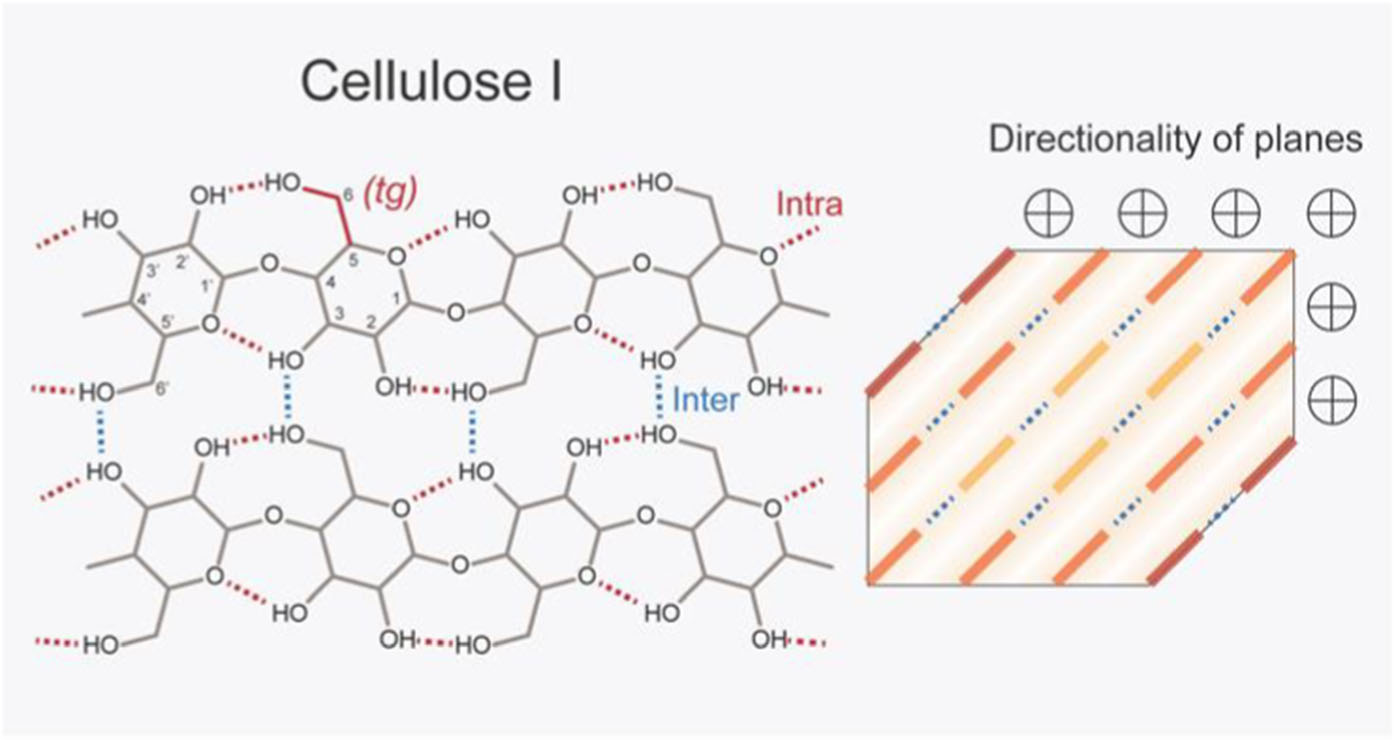
\includegraphics[width=0.96\textwidth]{cellulose_structure/cellulose_hydrogen_bonding_pattern_i.png}
        \subcaption{}
    \end{subfigure}
    \begin{subfigure}[b]{0.48\textwidth}
        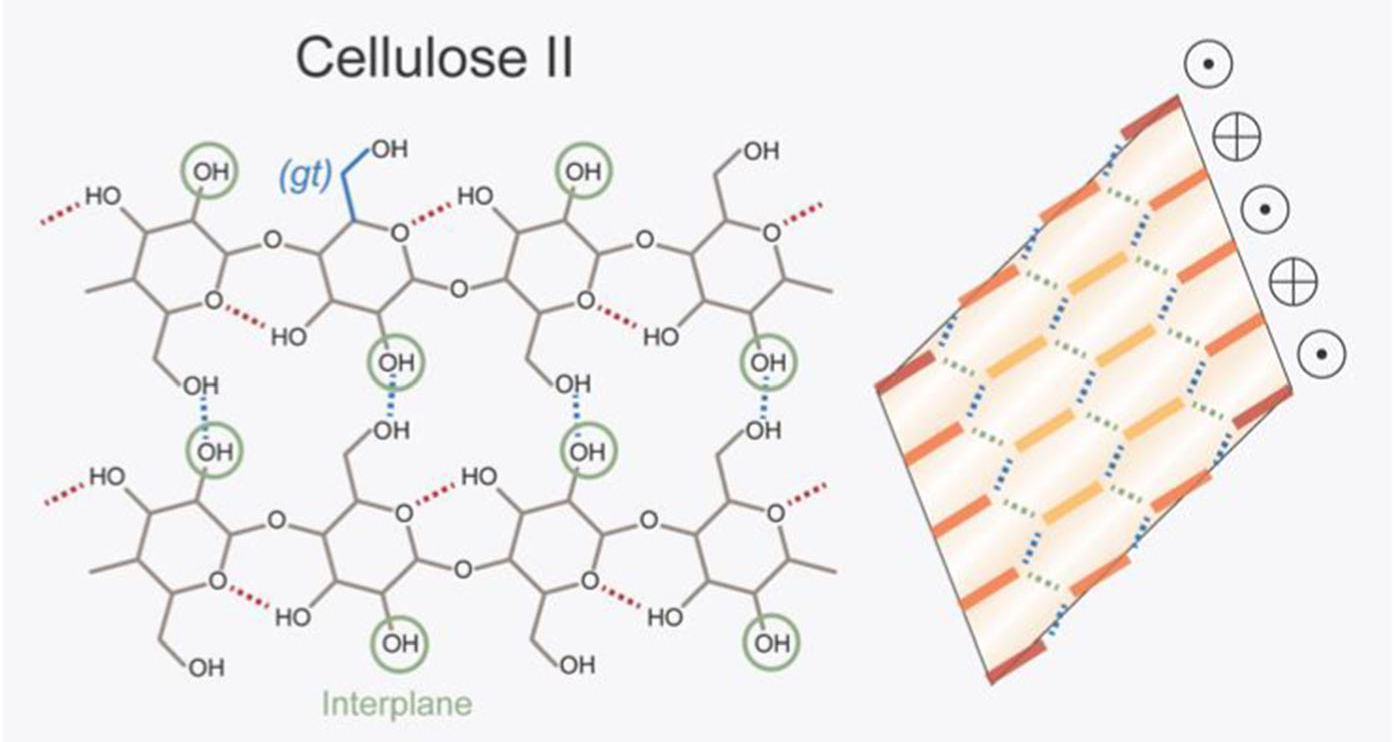
\includegraphics[width=0.96\textwidth]{cellulose_structure/cellulose_hydrogen_bonding_pattern_ii.png}
        \subcaption{}
    \end{subfigure}
    \\
    \begin{subfigure}[b]{0.28\textwidth}
        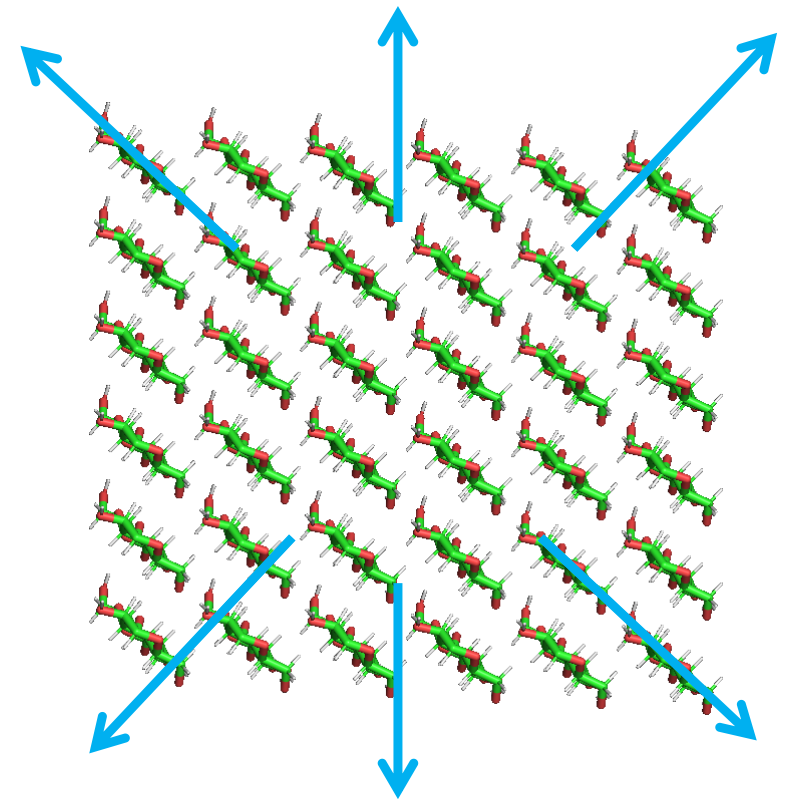
\includegraphics[width=0.96\textwidth]{cellulose_structure/characteristic_directions_i.png}
        \subcaption{}
    \end{subfigure}
    \hspace{0.20\textwidth}
    \begin{subfigure}[b]{0.28\textwidth}
        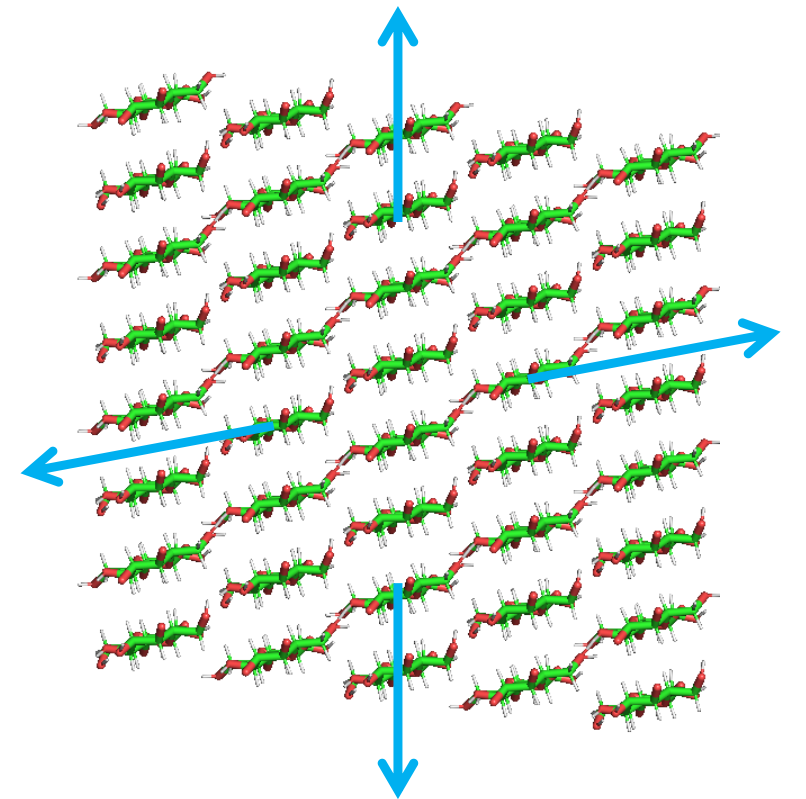
\includegraphics[width=0.96\textwidth]{cellulose_structure/characteristic_directions_ii.png}
        \subcaption{}
    \end{subfigure}
    \captionsetup{font=scriptsize}
    \caption{
    Cellulose nanocrystal arrangement patterns\cite{wohlert2022cellulose} and characteristic directions.
    (a) Arrangement pattern of Type I and (b) Type II cellulose nanocrystals.
    This study focuses on the two most common arrangement configurations, Type I and Type II, where Type I nanocrystals widely exist in plants and are also known as natural cellulose crystals.
    The difference between the two arrangements lies in the direction and arrangement interval of the side-chain hydroxyl groups, where the Type I nanocrystals is tg only and Type II is an alternating arrangement of tg and gt.
    Type I nanocrystals have more intrachain hydrogen bonds, while Type II with gt-type stress more on interchain hydrogen bonds.
    Unless explicitly specified, the cellulose nanocrystals mentioned in this study refer to Type I($\beta$) nanocrystals.
    (b) Characteristic directions of Type I and Type II considered in this study.
    Based on the hydrogen bonding patterns of Type I and Type II, three or two characteristic directions are considered in this study.
    For Type I, they were named as Vertical, Horizontal and Slant; for Type II, they were named as Vertical and Slant, which are also the direction relative to the the hydrogen bonding layers.
    }
    \label{fig:arrangement_patterns_and_characteristic_directions}
\end{figure}

\section*{Results}
\addtocounter{section}{1}
\setcounter{subsection}{0}
\addcontentsline{toc}{section}{\protect\numberline{}Results}\indent

\subsection{Anisotropic Mechanical Properties of Cellulose Nanocrystals}\indent

\subsubsection{Cellulose Nanocrystals Type I}\indent

According to the experimental data measured by Yoshiharu Nishiyama et al.\cite{nishiyama2002crystal}, the three characteristic dimensions of the cellulose nanocrystal lattice are a=0.778~nm, b=0.820~nm , c=1.038~nm, and the angle between the horizontal and vertical sides of the lattice is 96.55$^\circ$.
According to the data measured by Paul Langan et al. using X-ray technology\cite{langan2001x}, the three characteristic dimensions of the Type II cellulose nanocrystal lattice are a=0.810~nm, b=0.903~nm, and c=1.031~nm, and the angle between the transverse and longitudinal sides of the lattice is 117.10$^{\circ}$.
Based on these data, all atom models of Type I and Type II were constructed and relaxed for further stretch simulations, as shown in Figure \ref{fig:cellulose_nanocrystal_structure_and_models} and Figure \ref{fig:cellulose_nanocrystal_ii_structure_and_models}.

As shown in Figure \ref{fig:cellulose_nanocrystal_relaxations} and Figure \ref{fig:cellulose_nanocrystal_ii_relaxations}, the structures of the different arrangement models did not undergo significant structural changes after energy minimization and relaxation processes.
The presented models in these figures were processed for periodicity using the "nojump" method, meaning the coordinates of atoms do not change significantly relative to the initial structure by crossing periodic boundaries.
Therefore, the sliding of sheets in the vertical and horizontal models corresponds to actual displacement rather than display issues; this phenomenon also helps explain that the van der Waals interaction between sheets of cellulose nanocrystals is weaker than the hydrogen bonding within the sheets.
The RMSD (root mean square deviation) curves during relaxation quantitatively demonstrate the structural stability during the process.

\begin{figure}[htbp]
    \centering
    \scriptsize
    \begin{minipage}[b]{0.20\textwidth}
        \centering
        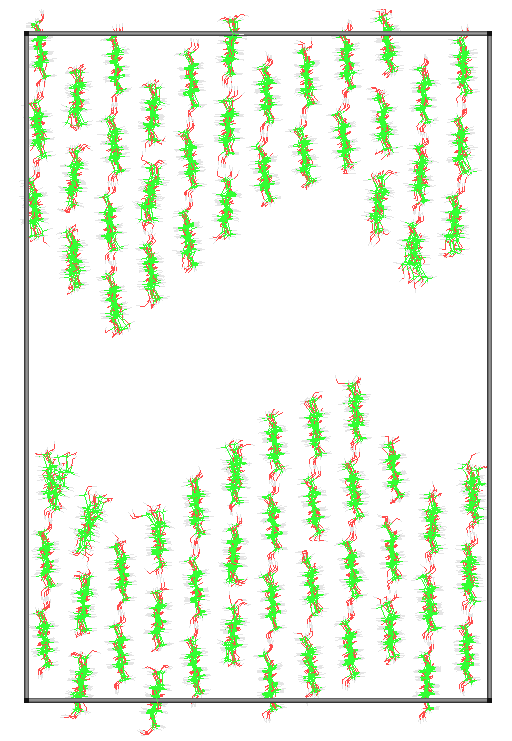
\includegraphics[width=0.96\textwidth]{cellulose_simulation_nanocrystal_i/fracture_vertical.png}
        \\
        Vertical
    \end{minipage}
    \begin{minipage}[b]{0.25\textwidth}
        \centering
        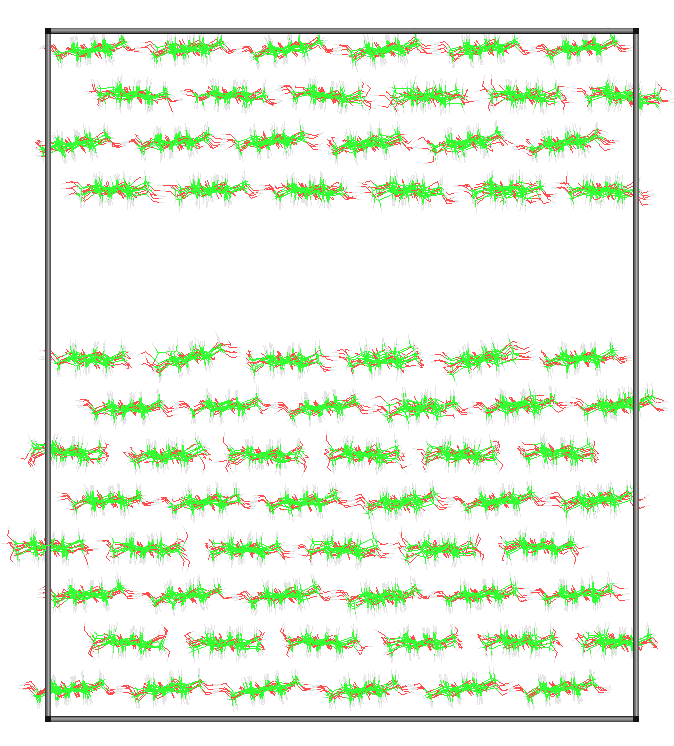
\includegraphics[width=0.96\textwidth]{cellulose_simulation_nanocrystal_i/fracture_horizontal.png}
        \\
        Horizontal
    \end{minipage}
    \begin{minipage}[b]{0.24\textwidth}
        \centering
        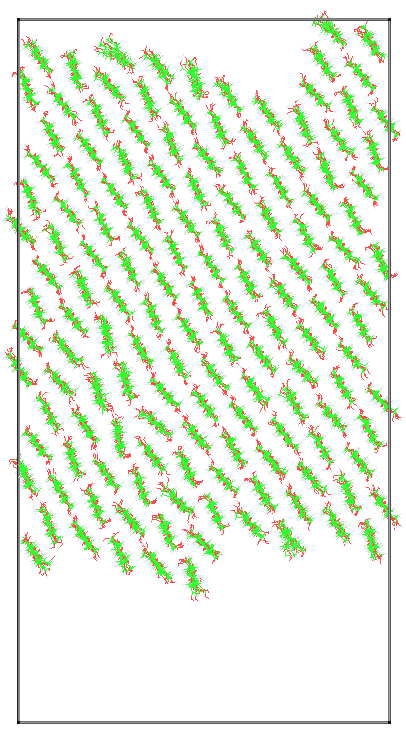
\includegraphics[width=0.96\textwidth]{cellulose_simulation_nanocrystal_i/fracture_slant.png}
        \\
        Slant
    \end{minipage}
    \captionsetup{font=scriptsize}
    \caption{
    Fracture behaviors of cellulose nanocrystals Type I.
    The vertical and horizontal models exhibited brittle fractures, while shear failure characterized by frictional sliding was presented by the slant model.
    The friction and overall rotation also illustrated the different strength of hydrogen bonding within a layer and van der Waals interactions between layers.
    }
    \label{fig:cellulose_nanocrystal_fractures}
\end{figure}

As shown by Figure \ref{fig:cellulose_nanocrystal_fractures}, the vertical and horizontal models exhibit the expected brittle fracture behavior, while significant relative sliding between layers occurred in the slant model, leading to a rotation of the overall crystal sheets after sliding.
In subsequent sections, this phenomenon will be referred to as frictional sliding, which is further shown in Figure \ref{fig:cellulose_nanocrystal_stretch_transitions_and_direction_angle}.

The specific data for stress, strain energy, hydrogen bond number, and potential energy during the tension of the vertical, horizontal, and slant models are shown in Figure \ref{fig:cellulose_nanocrystal_stretch_collection_and_speed_dependency} and Figure \ref{fig:cellulose_nanocrystal_stretch_hydrogen_bond_number_and_energy}.
From the perspectives of strength (maximum stress) and strain energy (maximum strain energy), the simulation data correspond to the strength of hydrogen bonding and van der Waals interactions.
The strength of the vertical model, where hydrogen bonding plays a dominant role also corresponds to the highest strength among the three arrangements;
Meanwhile, the slant arrangement model, affected by both hydrogen bonding and van der Waals interactions, exhibits the unique frictional sliding phenomenon, possessing the highest toughness and ductility despite having lower strength.
During the stretches of the three models, the number of hydrogen bonds in the horizontal model did not change significantly (the number of hydrogen bonds shown is the change relative to each minimum for comparison),
while a significant decrease in hydrogen bonds was observed in the vertical and slant models involving sheet fracture, reflecting the close correlation between hydrogen bonds and mechanical behavior.
However, the number of hydrogen bonds in the slant model gradually recovered after the decrease, which should be related to the hydrogen bond network reconstruction during the frictional sliding of the slant model, which also explains the higher toughness of the slant model from another perspective.

\begin{figure}[htbp]
    \centering
    \begin{subfigure}[b]{0.96\textwidth}
        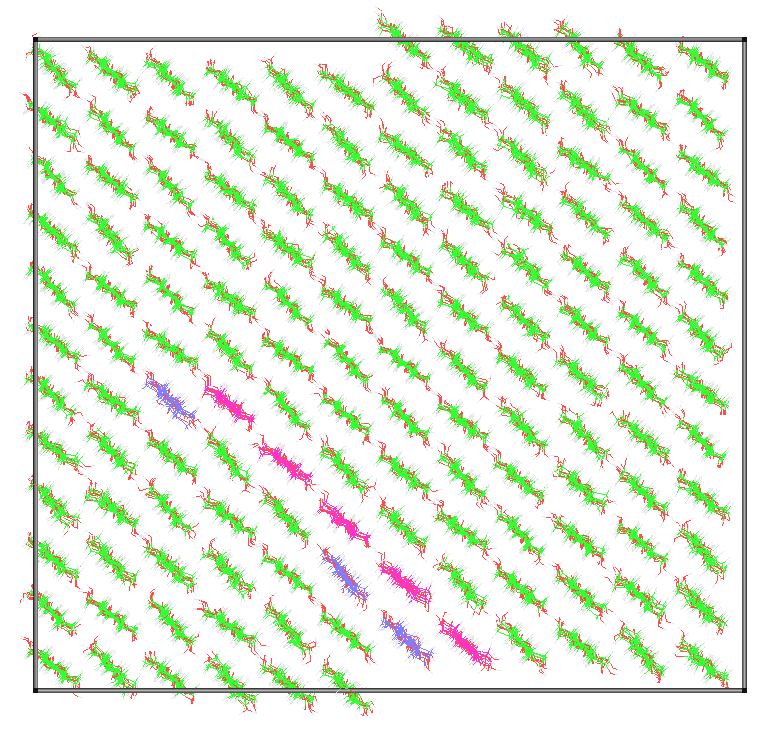
\includegraphics[width=0.24\textwidth]{cellulose_simulation_nanocrystal_i/stretch_frame_slant_5.png}
        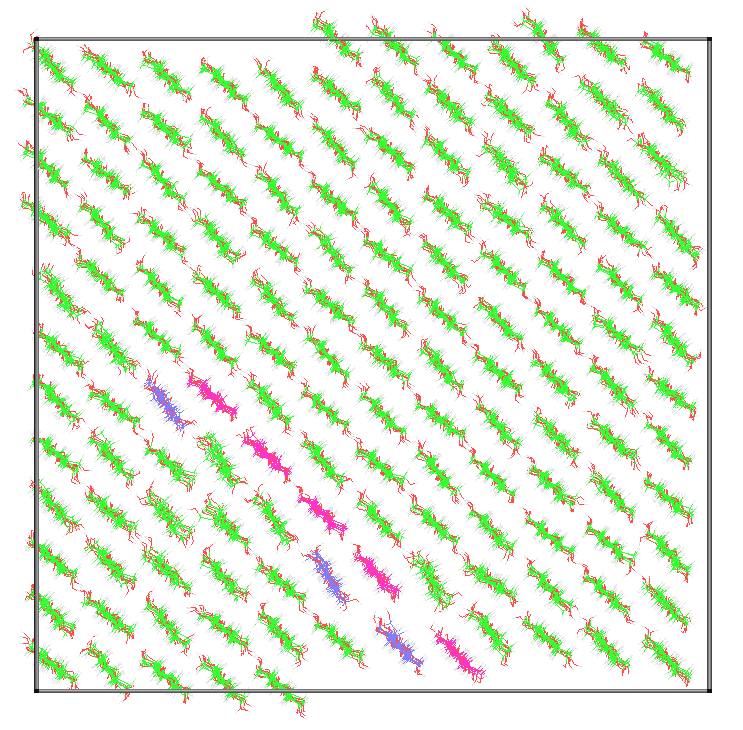
\includegraphics[width=0.24\textwidth]{cellulose_simulation_nanocrystal_i/stretch_frame_slant_7.png}
        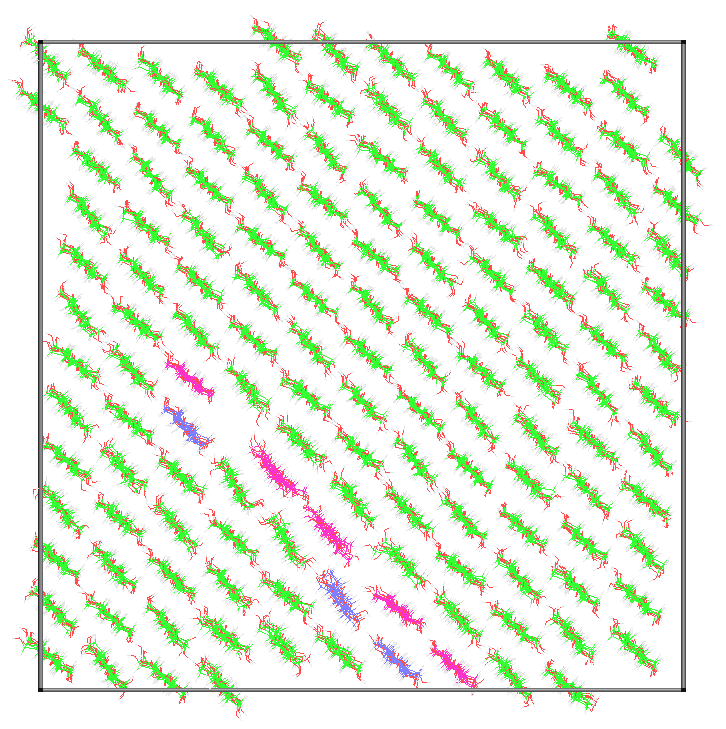
\includegraphics[width=0.24\textwidth]{cellulose_simulation_nanocrystal_i/stretch_frame_slant_8.png}
        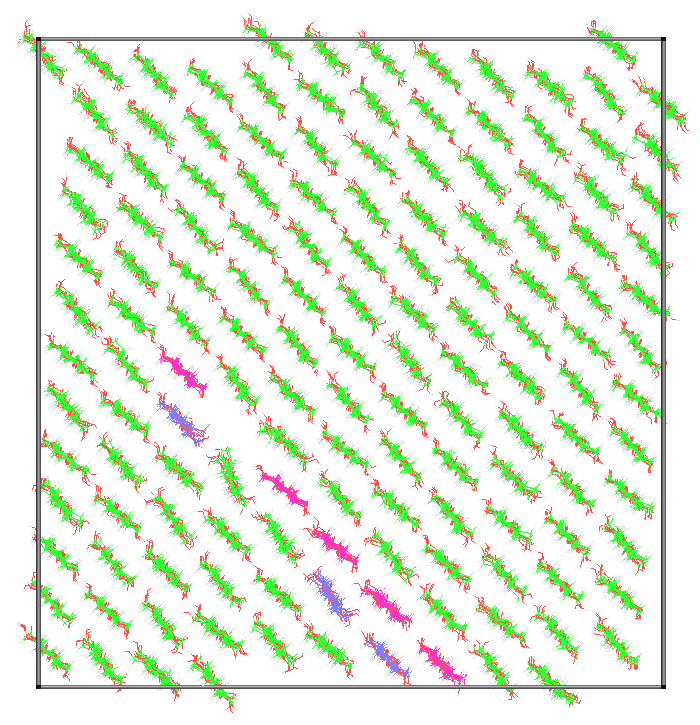
\includegraphics[width=0.24\textwidth]{cellulose_simulation_nanocrystal_i/stretch_frame_slant_9.png}
        \\
        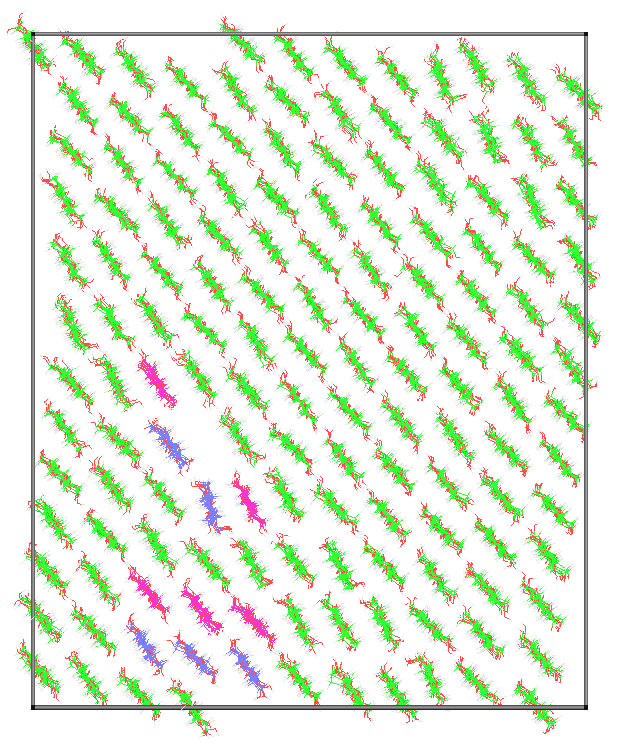
\includegraphics[width=0.24\textwidth]{cellulose_simulation_nanocrystal_i/stretch_frame_slant_16.png}
        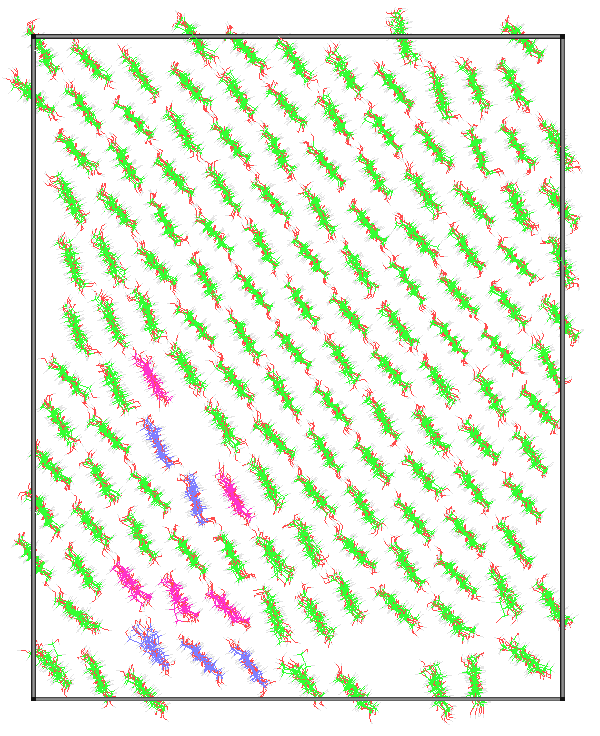
\includegraphics[width=0.24\textwidth]{cellulose_simulation_nanocrystal_i/stretch_frame_slant_19.png}
        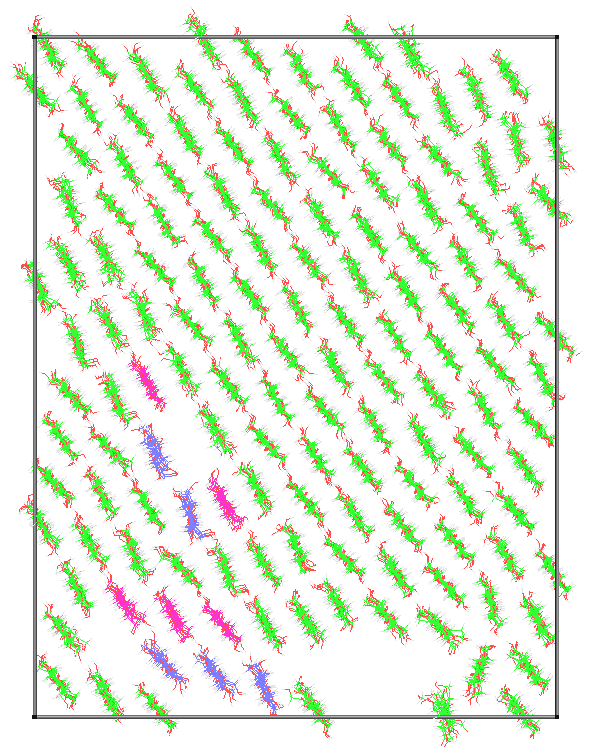
\includegraphics[width=0.24\textwidth]{cellulose_simulation_nanocrystal_i/stretch_frame_slant_20.png}
        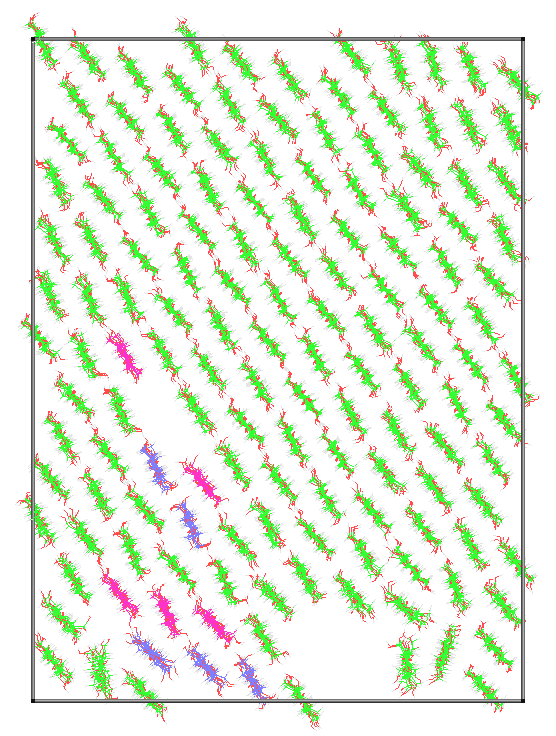
\includegraphics[width=0.24\textwidth]{cellulose_simulation_nanocrystal_i/stretch_frame_slant_21a.png}
        \subcaption{}
    \end{subfigure}
    \\
    \begin{subfigure}[b]{0.96\textwidth}
        \centering
        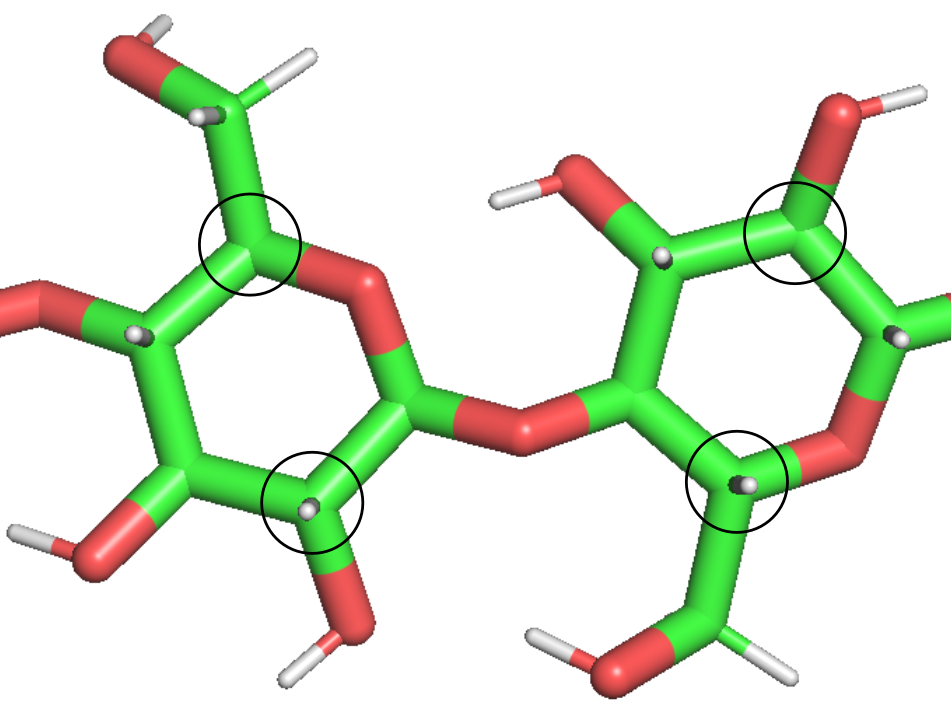
\includegraphics[width=0.32\textwidth]{cellulose_simulation_nanocrystal_i/direction_angle_atom.png}
        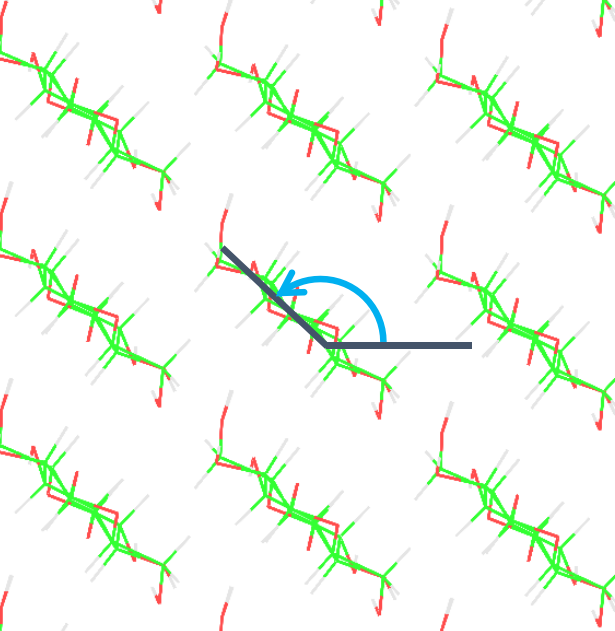
\includegraphics[width=0.24\textwidth]{cellulose_simulation_nanocrystal_i/direction_angle_definition.png}
        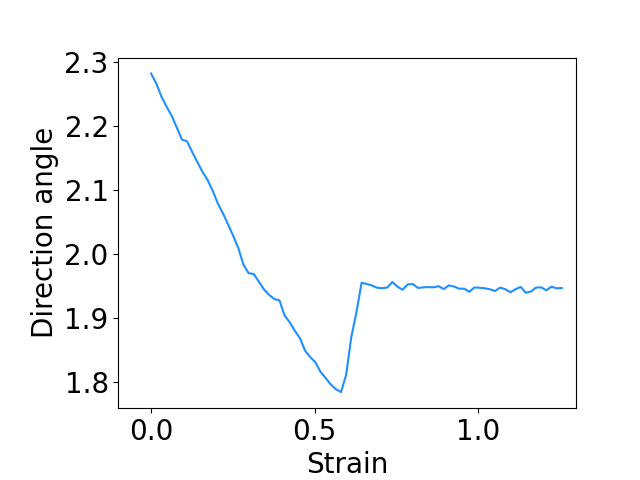
\includegraphics[width=0.40\textwidth]{cellulose_simulation_nanocrystal_i/stretch_direction_angle_slant.png}
        \subcaption{}
    \end{subfigure}
    \captionsetup{font=scriptsize}
    \caption{
    Structure transitions of cellulose nanocrystals Type I during stretches.
    (a) Key frames of the frictional sliding phenomenon in the slant model.
    Relative frictional sliding between adjacent layers was an important failure phenomenon in the slant model.
    (b) Definition of the direction angle and the direction angle curve during the tension of the slant model.
    To quantitatively characterize the frictional sliding and the resulting rotation in the slant model, the direction angle was introduced and defined as the projection angle of carbon atoms on the ring.
    For the entire model, its direction angle was the average of all residues.
    The direction angle curve effectively illustrated the frictional sliding and rotation of the model, and the later recovery corresponds to the rebound after fracture.
    }
    \label{fig:cellulose_nanocrystal_stretch_transitions_and_direction_angle}
\end{figure}

The dominant role of Coulomb interaction in the vertical models is further illustrated by the potential energy data (the potential energy data is relative to its respective minimums for easier comparison) in Figure \ref{fig:cellulose_nanocrystal_ii_stretch_hydrogen_bond_number_and_energy}.
By comparing the delta in Coulomb potential energy during stretches, the vertical model is the only case where Coulomb potential energy increased.
That means, only in the vertical model, the Coulomb interaction played an important role in resisting stretches.
Besides, increased van der Waals potential energy were observed in all of the three models, particularly for slant model, which is related to its highest toughness.

Regarding the unique frictional sliding phenomenon in cellulose nanocrystals, transition key frames are shown in Figure \ref{fig:cellulose_nanocrystal_stretch_transitions_and_direction_angle}.
The frictional sliding in the slant model began with the fracture of one layer of cellulose nanocrystals; after the fracture, significant sliding on the interface between both sides can be observed, and the fractured edges may reconnect with each other after overall rotations.
To quantitatively describe the rotation of layers, the direction angle was defined (Figure \ref{fig:cellulose_nanocrystal_stretch_transitions_and_direction_angle}).
The direction angle is the projection angle on the cross section, between the horizontal axis and two carbon atoms on a residue ring.
And the direction angle of a frame is the average of all the residues.
The recovery at the end of the direction angles curve, corresponds to the rebound after final fractures of the slant model.

Subsequently, to reduce the impact of individual cases and simulation randomness and to consider the effect of stretch speed, 100 replica simulations were performed for all of the three models at varying stretch speeds.
The stretch speeds considered include 0.1~nm/ns, 1.0~nm/ns, 2.0~nm/ns, 4.0~nm/ns, 10.0~nm/ns, 20.0~nm/ns, and 40.0~nm/ns.
The replica number of simulations at 0.1 nm/ns was 10 owing to the computational expenses.
As shown by the stress-strain curves and strain energy curves of 100 replica stretches at 10.0 nm/ns (Figure \ref{fig:cellulose_nanocrystal_stretch_collection_and_speed_dependency}), the mechanical performances of cellulose nanocrystals in the three characteristic directions are stable.
The brittleness of the vertical and horizontal models and the toughness of the slant model were all confirmed through replica simulations.
After considering all the strength and toughness performances across varying stretch speeds, it can be confirmed that the mechanical properties of cellulose nanocrystals Type I are stable within the considered range of stretch speeds.

\begin{figure}[htbp]
    \centering
    \scriptsize
    \begin{subfigure}[b]{0.96\textwidth}
        \centering
        \begin{minipage}[b]{0.32\textwidth}
            \centering
            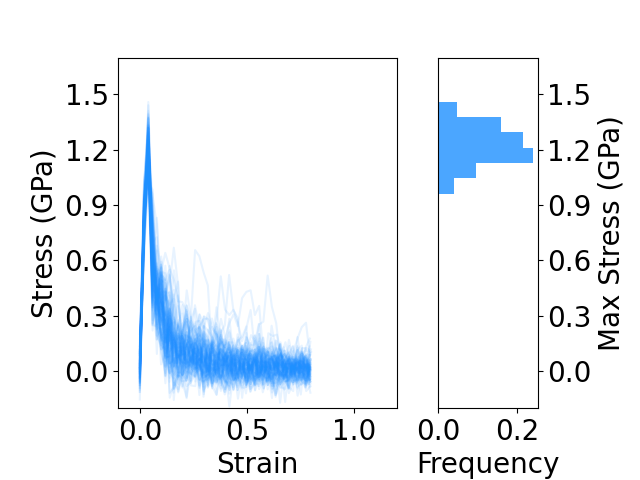
\includegraphics[width=0.96\textwidth]{cellulose_simulation_nanocrystal_i/stretch_stress_strain_collection_vertical_10.0.png}
        \end{minipage}
        \begin{minipage}[b]{0.32\textwidth}
            \centering
            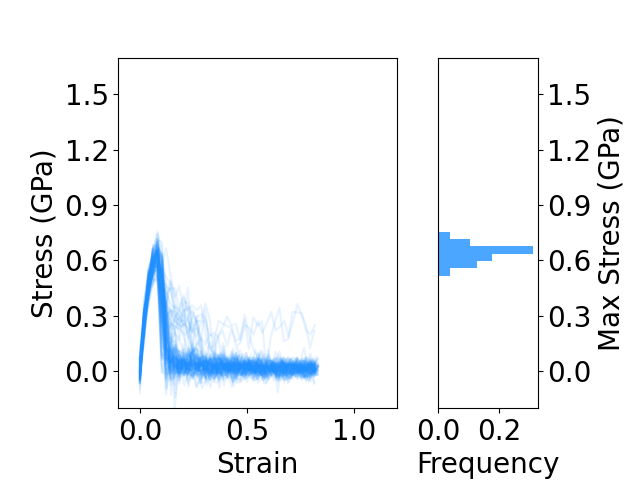
\includegraphics[width=0.96\textwidth]{cellulose_simulation_nanocrystal_i/stretch_stress_strain_collection_horizontal_10.0.png}
        \end{minipage}
        \begin{minipage}[b]{0.32\textwidth}
            \centering
            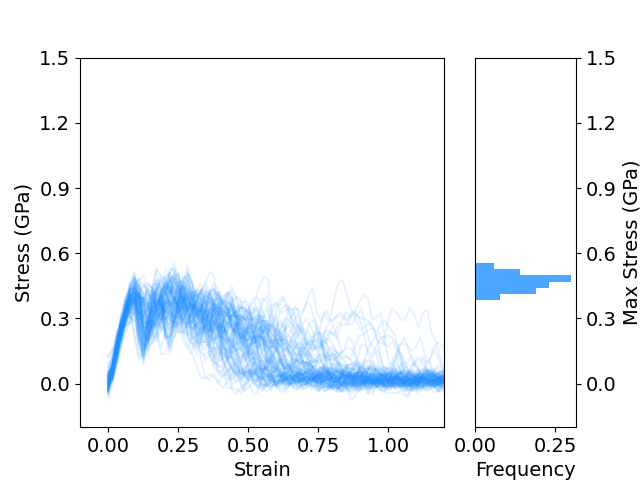
\includegraphics[width=0.96\textwidth]{cellulose_simulation_nanocrystal_i/stretch_stress_strain_collection_slant_10.0.png}
        \end{minipage}
        \subcaption{}
    \end{subfigure}
    \\
    \begin{subfigure}[b]{0.96\textwidth}
        \centering
        \begin{minipage}[b]{0.32\textwidth}
            \centering
            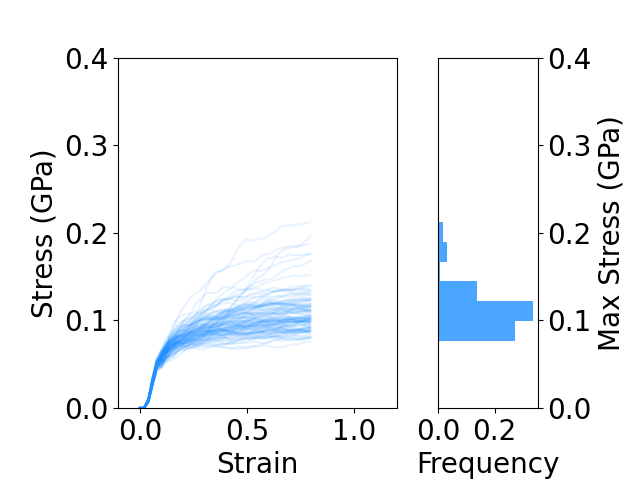
\includegraphics[width=0.96\textwidth]{cellulose_simulation_nanocrystal_i/stretch_strain_energy_collection_vertical_10.0.png}
            \\
            Vertical
        \end{minipage}
        \begin{minipage}[b]{0.32\textwidth}
            \centering
            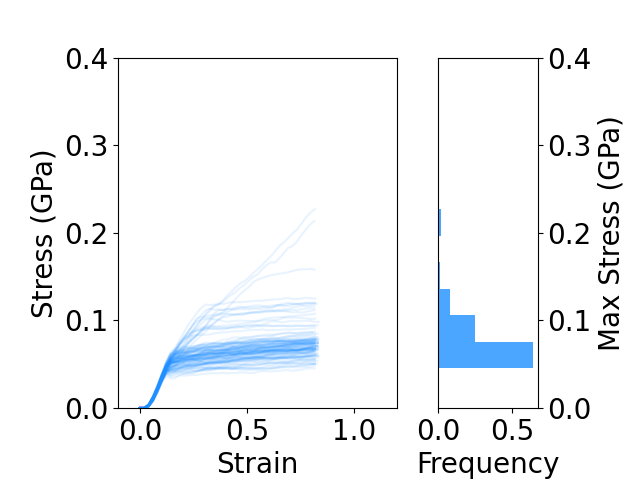
\includegraphics[width=0.96\textwidth]{cellulose_simulation_nanocrystal_i/stretch_strain_energy_collection_horizontal_10.0.png}
            \\
            Horizontal
        \end{minipage}
        \begin{minipage}[b]{0.32\textwidth}
            \centering
            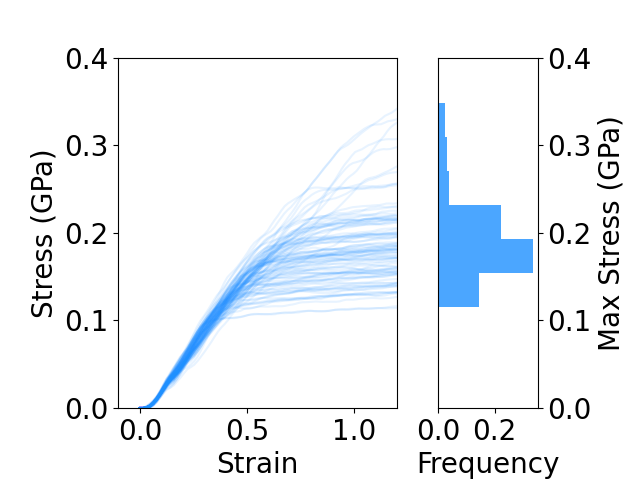
\includegraphics[width=0.96\textwidth]{cellulose_simulation_nanocrystal_i/stretch_strain_energy_collection_slant_10.0.png}
            \\
            Slant
        \end{minipage}
        \subcaption{}
    \end{subfigure}
    \\
    \begin{subfigure}[b]{0.96\textwidth}
        \centering
        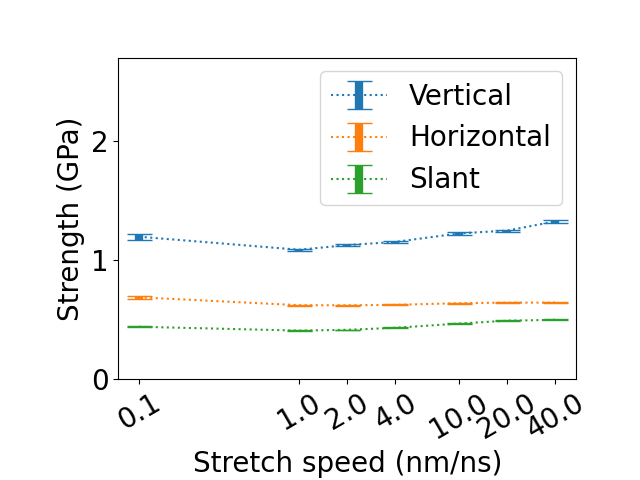
\includegraphics[width=0.48\textwidth]{cellulose_simulation_nanocrystal_i/stretch_strength_with_speed.png}
        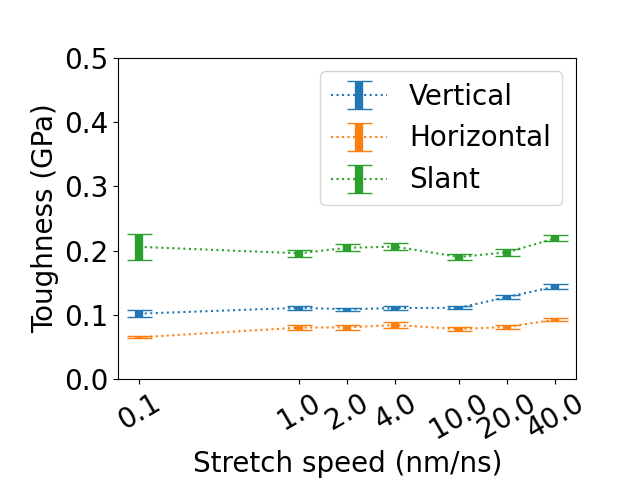
\includegraphics[width=0.48\textwidth]{cellulose_simulation_nanocrystal_i/stretch_toughness_with_speed.png}
        \subcaption{}
    \end{subfigure}
    \captionsetup{font=scriptsize}
    \caption{
    Stress curves and deviations of cellulose nanocrystals Type I mechanical properties under varying stretch speeds.
    (a) Stress-strain curves and corresponding maximum stress distributions for vertical, horizontal, and slant models under 100 replica simulations at 10.0 nm/ns.
    (b) Strain energy curves and corresponding maximum strain energy distributions for vertical, horizontal, and slant models under 100 replica simulations at 10.0 nm/ns.
    (c) Mechanical properties of vertical, horizontal, and slant models with stretch speed.
    Each data point represents the mean value plus or minus one standard error.
    Except for 0.1~nm/ns, which was only repeated 10 times, all other stretch speed data are the results of 100 replica simulations with distributions similar to those at 10.0 nm/ns.
    These data indicate that the mechanical properties of the cellulose nanocrystals Type I do not change significantly with stretch speed within the considered range.
    }
    \label{fig:cellulose_nanocrystal_stretch_collection_and_speed_dependency}
\end{figure}

\subsubsection{Cellulose Nanocrystals Type II}\indent

Another widely available cellulose nanocrystal configuration with better thermal stability is called Type II\cite{malaspina2019molecular}.
In addition to the lattice dimensions, Type II cellulose nanocrystals have another significant difference from Type I: the orientation of the cellulose residues.
In Type I, all side chains are the tg type pointing to one direction; while in Type II nanocrystals, the tg and gt types are connected alternately.
Corresponding to Figure \ref{fig:cellulose_nanocrystal_ii_structure_and_models}, the side chains corresponding to the gt type point to the right, and those of the tg type point to the left.
The core difference between gt and tg types lies in the arrangement pattern of hydrogen bonds between side chain hydroxyl groups; the gt type forms more intra chain hydrogen bonds, and the tg type emphasizes more on inter chain hydrogen bonds.
Cellulose nanocrystals Type II do not have a significant laminar structure and only have two characteristic directions, corresponding to the vertical and slant model respectively.

\begin{figure}[htbp]
    \centering
    \scriptsize
    \begin{minipage}[b]{0.15\textwidth}
        \centering
        
\includegraphics[width=0.96\textwidth]{cellulose_simulation_nanocrystal_ii/fracture_vertical.png}
        \\
        Vertical
    \end{minipage}
    \hspace{0.12\textwidth}
    \begin{minipage}[b]{0.18\textwidth}
        \centering
        
\includegraphics[width=0.96\textwidth]{cellulose_simulation_nanocrystal_ii/fracture_slant.png}
        \\
        Slant
    \end{minipage}
    \hspace{0.16\textwidth}
    \begin{minipage}[b]{0.12\textwidth}
        \centering
        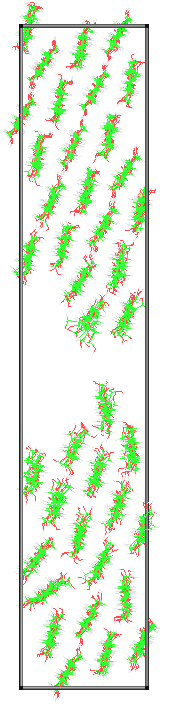
\includegraphics[width=0.96\textwidth]{cellulose_simulation_nanocrystal_ii/fracture_slant_tough.png}
        \\
        Slant Tough
    \end{minipage}
    \captionsetup{font=scriptsize}
    \caption{
    Fracture behaviors of cellulose nanocrystals Type II.
    The vertical models exhibited brittle fractures, while the slant models may undergo structural reorganization during the stretching process.
    The slant model may also exhibit brittle fractures, or form a laminar structure similar to Type I with higher toughness (marked as ``Slant Tough'', and the image was scaled to be much smaller comparing to ``Slant'').
    This phenomenon was an configuration restructure mechanism induced by external loads, may be helpful to the extraction and material design for cellulose nanocrystals.
    }
    \label{fig:cellulose_nanocrystal_ii_fractures}
\end{figure}

Type II fracture behaviors (Figure \ref{fig:cellulose_nanocrystal_ii_fractures} and Figure \ref{fig:cellulose_nanocrystal_ii_stretch_transitions}) and the mechanical properties deviations (Figure \ref{fig:cellulose_nanocrystal_ii_stretch_collection_and_speed_dependency}) significantly differ with Type I.
The slant model of Type II nanocrystals can exhibit brittle behavior and lower toughness, or it can undergo restructure during stretch, exhibiting higher toughness.
During the stretching process, the structure of Type II cellulose crystals may transform into a laminar structure similar to the Type I and achieve higher toughness.
This is a phenomenon of configuration transformation mediated by mechanical loading.

Figure \ref{fig:cellulose_nanocrystal_ii_stretch_transitions} provides key frames of the two typical stretch transitions for slant models.
From the perspective of restructure, the difference between the cases of lower and higher toughness in the slant models is whether the fractures happened early in a specific area or not.
However, in both cases, the subsequent structures would restructure to be laminar, similar to that of the Type I slant models.
This special deformation was also confirmed in larger models (the length and width of cross section were both doubled, Figure \ref{fig:cellulose_nanocrystal_ii_larger_stretch_transitions}).

\begin{figure}[htbp]
    \centering
    \begin{subfigure}[b]{0.44\textwidth}
        \centering
        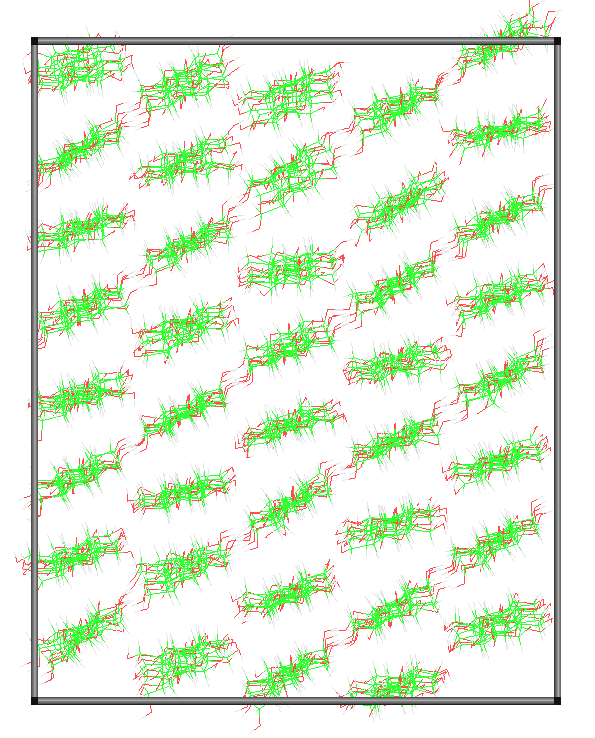
\includegraphics[width=0.24\textwidth]{cellulose_simulation_nanocrystal_ii/stretch_frame_slant_14.png}
        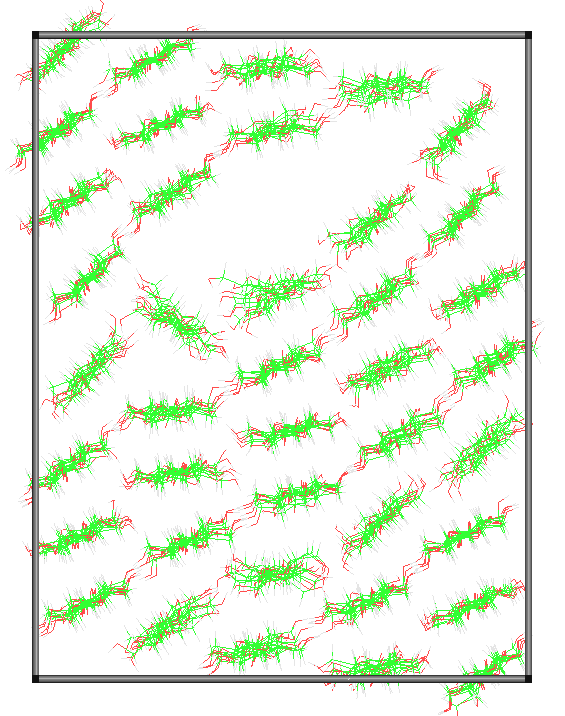
\includegraphics[width=0.24\textwidth]{cellulose_simulation_nanocrystal_ii/stretch_frame_slant_15.png}
        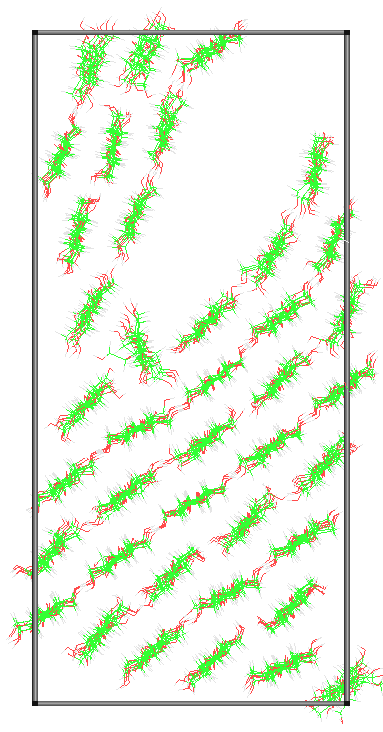
\includegraphics[width=0.24\textwidth]{cellulose_simulation_nanocrystal_ii/stretch_frame_slant_41.png}
        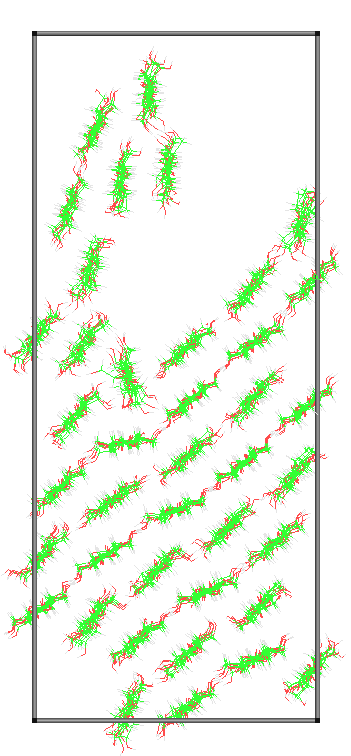
\includegraphics[width=0.24\textwidth]{cellulose_simulation_nanocrystal_ii/stretch_frame_slant_54.png}
        \subcaption{}
    \end{subfigure}
    \hspace{0.10\textwidth}
    \begin{subfigure}[b]{0.44\textwidth}
        \centering
        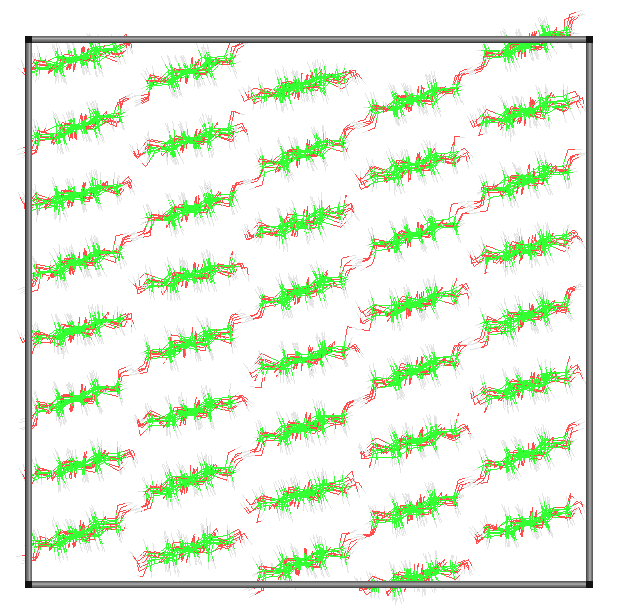
\includegraphics[width=0.24\textwidth]{cellulose_simulation_nanocrystal_ii/stretch_frame_slant_tough_0.png}
        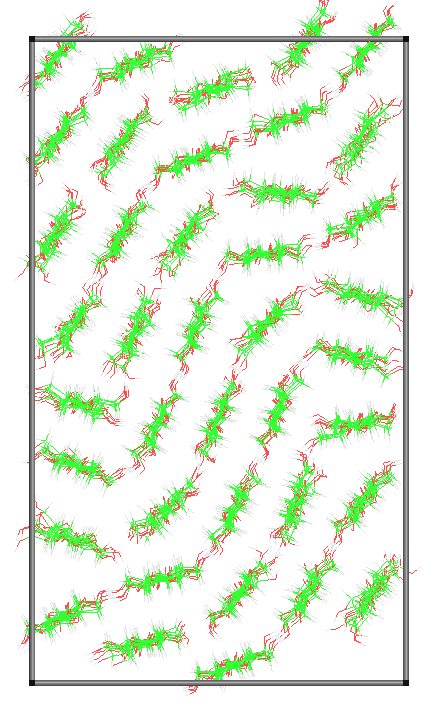
\includegraphics[width=0.24\textwidth]{cellulose_simulation_nanocrystal_ii/stretch_frame_slant_tough_24.png}
        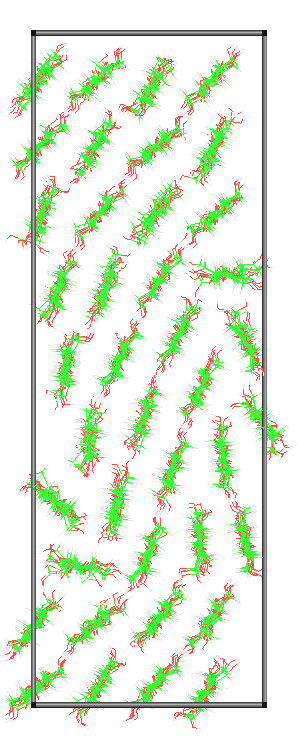
\includegraphics[width=0.24\textwidth]{cellulose_simulation_nanocrystal_ii/stretch_frame_slant_tough_48.png}
        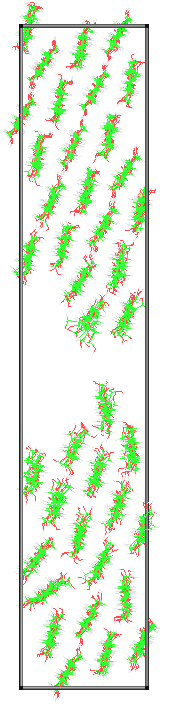
\includegraphics[width=0.24\textwidth]{cellulose_simulation_nanocrystal_ii/stretch_frame_slant_tough_96.png}
        \subcaption{}
    \end{subfigure}
    \captionsetup{font=scriptsize}
    \caption{
    Structure transitions of cellulose nanocrystals Type II during stretches.
    (a) (b) Key frames of the slant models from two typical fracture behaviors.
    Different from the stable frictional sliding behavior of Type I, the slant model of Type II may undergo brittle fractures or restructure into a laminar arrangement similar to Type I.
    The restructure induced by loads with higher toughness corresponded to an overall frictions and rotations, rather than localized fractures.
    Both cases would restructure to be laminar and similar to that of the Type I slant models.
    }
    \label{fig:cellulose_nanocrystal_ii_stretch_transitions}
\end{figure}

The specific data for stress, strain energy, hydrogen bond number, and potential energy during the tension of the vertical, horizontal, and slant models are shown in Figure \ref{fig:cellulose_nanocrystal_ii_stretch_collection_and_speed_dependency} and Figure \ref{fig:cellulose_nanocrystal_ii_stretch_hydrogen_bond_number_and_energy}.
Proven by the data in figures, the vertical model of cellulose nanocrystals Type II is also dominated by hydrogen bonding, possessing higher strength than the slanted model.
And its higher strength corresponds to a greater increase in Coulomb potential energy.
Different from the Type I, the number of hydrogen bonds all decreased and Coulomb potential energies of Type II all increased, illustrating the crucial role of hydrogen bonds.
Although the all the van der Waals potential increased, the slant model with restructure and higher toughness, increased more in van der Waals potential energy.
In cellulose nanocrystals Type II, both Coulomb and Van der Waals interactions play important roles in resisting stretches.
The unique restructure phenomenon of the slant model is dependent on ideal crystal structure and periodicity, which would be further illustrated in later simulations with solvents around.

Considering the uniqueness of possible restructure, the replica simulations of speed dependency were also performed for the Type II, as shown in Figure \ref{fig:cellulose_nanocrystal_ii_stretch_collection_and_speed_dependency}.
The brittleness of the vertical model and the possible restructure of the slant model were all confirmed through replica simulations.
After considering all the strength and toughness performances across varying stretch speeds, it can be confirmed that the mechanical properties of cellulose nanocrystals Type II are stable within the considered range of stretch speeds.

\begin{figure}[htbp]
    \centering
    \scriptsize
    \begin{subfigure}[b]{0.96\textwidth}
        \centering
        \begin{minipage}[b]{0.32\textwidth}
            \centering
            
\includegraphics[width=0.96\textwidth]{cellulose_simulation_nanocrystal_ii/stretch_stress_strain_collection_vertical_10.0.png}
        \end{minipage}
        \begin{minipage}[b]{0.32\textwidth}
            \centering
            
\includegraphics[width=0.96\textwidth]{cellulose_simulation_nanocrystal_ii/stretch_stress_strain_collection_slant_10.0.png}
        \end{minipage}
        \begin{minipage}[b]{0.32\textwidth}
            \centering
            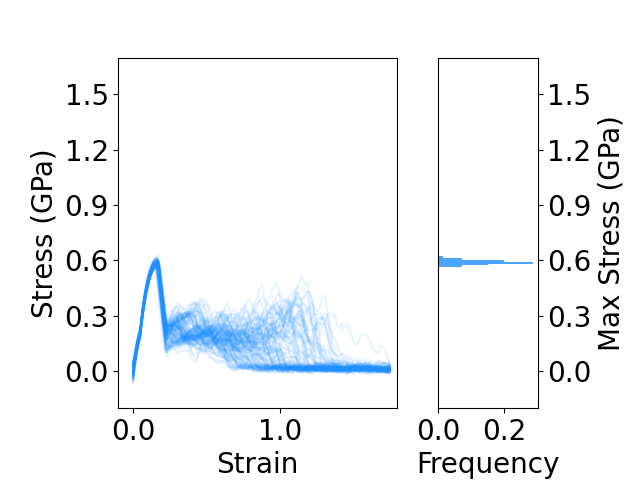
\includegraphics[width=0.96\textwidth]{cellulose_simulation_nanocrystal_ii/stretch_stress_strain_collection_slant_square_10.0.png}
        \end{minipage}
        \subcaption{}
    \end{subfigure}
    \\
    \begin{subfigure}[b]{0.96\textwidth}
        \centering
        \begin{minipage}[b]{0.32\textwidth}
            \centering
            
\includegraphics[width=0.96\textwidth]{cellulose_simulation_nanocrystal_ii/stretch_strain_energy_collection_vertical_10.0.png}
            \\
            Vertical
        \end{minipage}
        \begin{minipage}[b]{0.32\textwidth}
            \centering
            
\includegraphics[width=0.96\textwidth]{cellulose_simulation_nanocrystal_ii/stretch_strain_energy_collection_slant_10.0.png}
            \\
            Slant
        \end{minipage}
        \begin{minipage}[b]{0.32\textwidth}
            \centering
            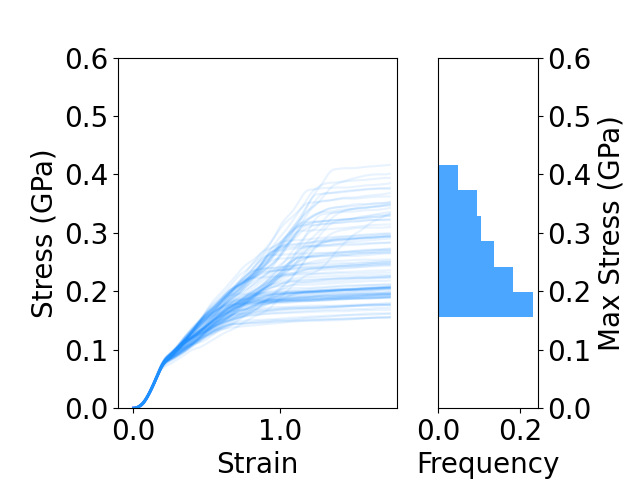
\includegraphics[width=0.96\textwidth]{cellulose_simulation_nanocrystal_ii/stretch_strain_energy_collection_slant_square_10.0.png}
            \\
            Slant (Larger)
        \end{minipage}
        \subcaption{}
    \end{subfigure}
    \\
    \begin{subfigure}[b]{0.96\textwidth}
        
\includegraphics[width=0.48\textwidth]{cellulose_simulation_nanocrystal_ii/stretch_strength_with_speed.png}
        
\includegraphics[width=0.48\textwidth]{cellulose_simulation_nanocrystal_ii/stretch_toughness_with_speed.png}
        \subcaption{}
    \end{subfigure}
    \captionsetup{font=scriptsize}
    \caption{
    Stress curves and deviations of cellulose nanocrystals Type II mechanical properties under varying stretch speeds.
    (a) Stress-strain curves and corresponding maximum stress distributions for vertical, slant, and larger size slant models under 100 replica simulations at 10.0 nm/ns.
    (b) Strain energy curves and corresponding maximum strain energy distributions for vertical, slant, and larger size slant models under 100 replica simulations at 10.0 nm/ns.
    (c) Mechanical properties of vertical, slant, and larger size slant models with stretch speed.
    Each data point represents the mean value plus or minus one standard error.
    Considering the deviation of the stress-strain curves of the slant model, simulation data from the larger size (double the width and height in the cross section) ware added.
    Except for 0.1 nm/ns, which was only repeated 10 times, all other stretch speed data are the results of 100 replica simulations with distributions similar to those at 10.0 nm/ns.
    These data indicate that the mechanical properties of the cellulose nanocrystals Type II do not change significantly with stretch speed within the considered range.
    }
    \label{fig:cellulose_nanocrystal_ii_stretch_collection_and_speed_dependency}
\end{figure}

\subsection{Size dependency and toughening mechanism}\indent

\subsubsection{Size dependency}\indent

According to data provided by Robert Sinko et al.\cite{sinko2014dimensions}, the mechanical properties of cellulose nanocrystals Type I are tightly related to their size.
When the size reaches a certain point, the mechanical performances of cellulose nanocrystals Type I tends to stabilize.
Our simulation results confirm this point as well, as shown in Figure \ref{fig:cellulose_nanocrystal_size_dependency}.
These models were ``square'', that means the length and width of its cross section is the same in terms of row and column number, such as 6$\times$6 and 12$\times$12.
The considered length here included 6, 9, 12, 18, 24, 36, and 64.
With a increasing size, the fracture strain (inferred from the fractures), strength, toughness, and the direction angle illustrated a stable decreasing tendency.

\begin{figure}[htbp]
    \centering
    \begin{subfigure}[b]{0.96\textwidth}
        \centering
        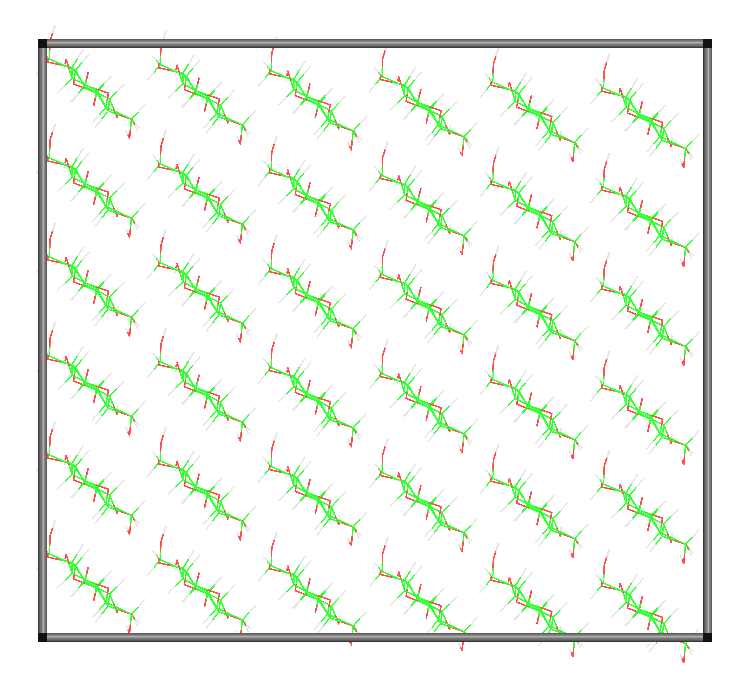
\includegraphics[width=0.12\textwidth]{cellulose_simulation_nanocrystal_different_size_i/model_36.png}
        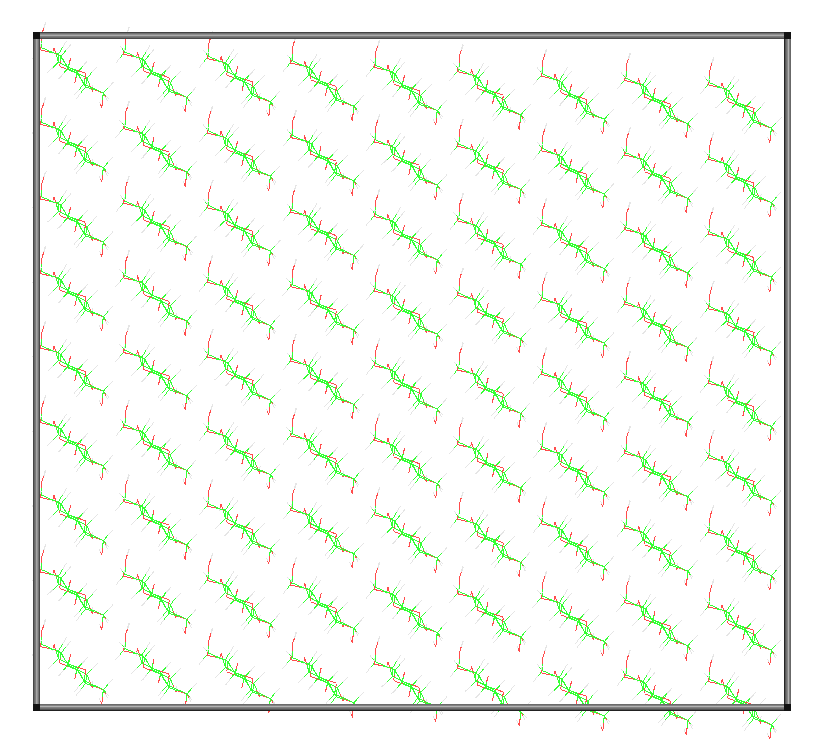
\includegraphics[width=0.12\textwidth]{cellulose_simulation_nanocrystal_different_size_i/model_81.png}
        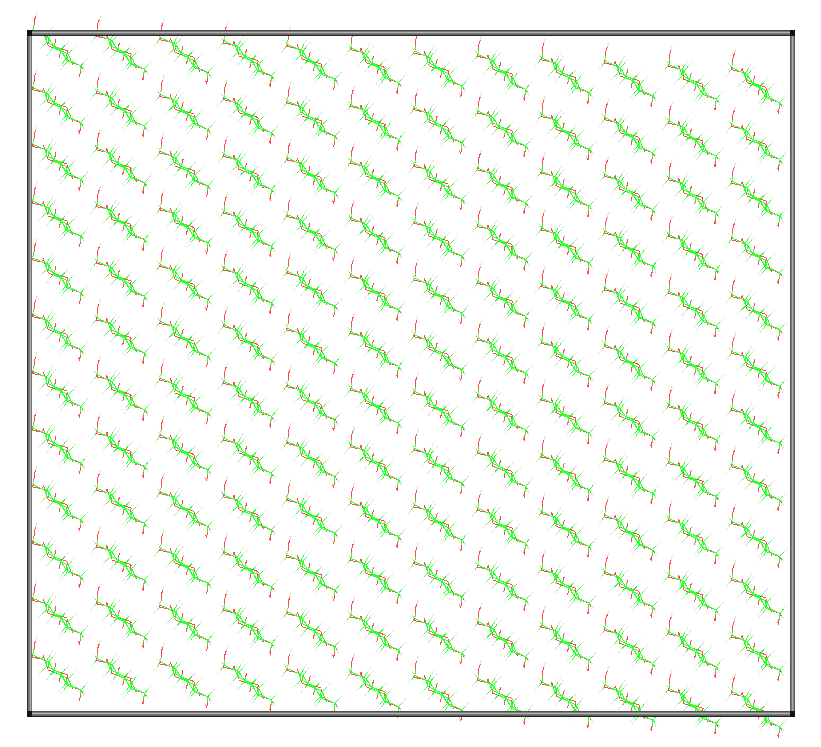
\includegraphics[width=0.12\textwidth]{cellulose_simulation_nanocrystal_different_size_i/model_144.png}
        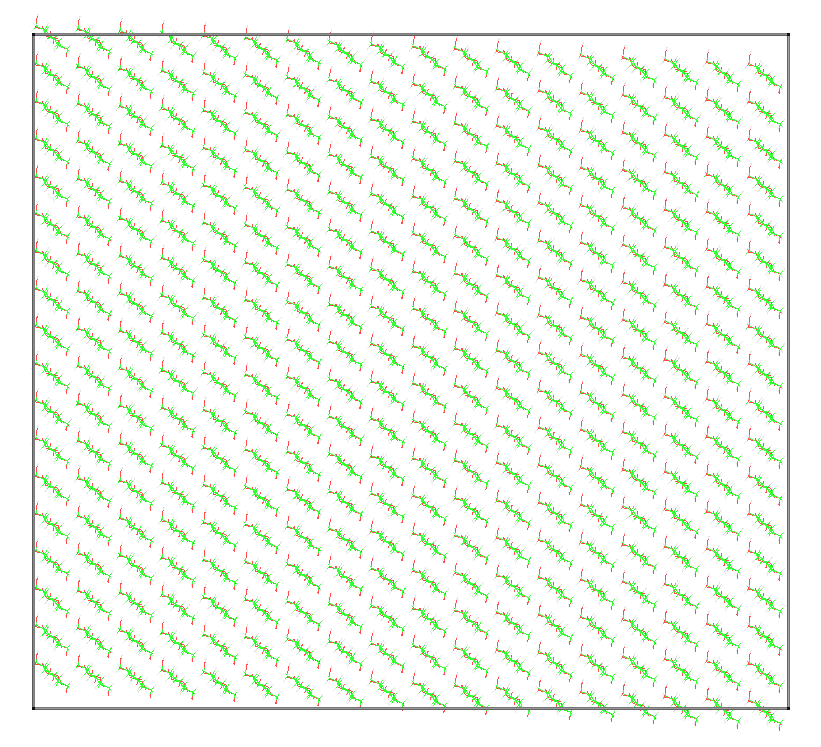
\includegraphics[width=0.12\textwidth]{cellulose_simulation_nanocrystal_different_size_i/model_324.png}
        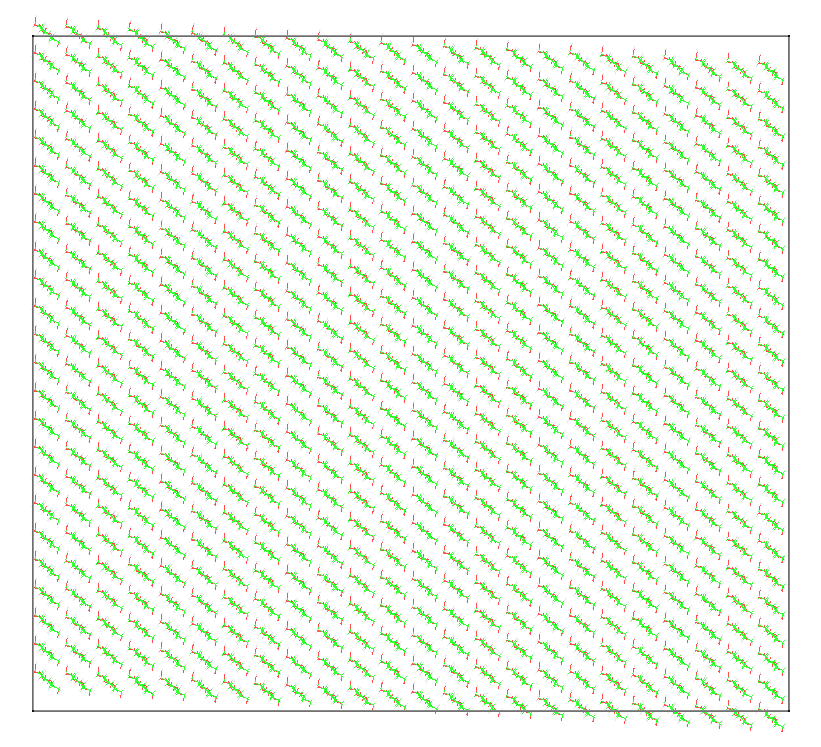
\includegraphics[width=0.12\textwidth]{cellulose_simulation_nanocrystal_different_size_i/model_576.png}
        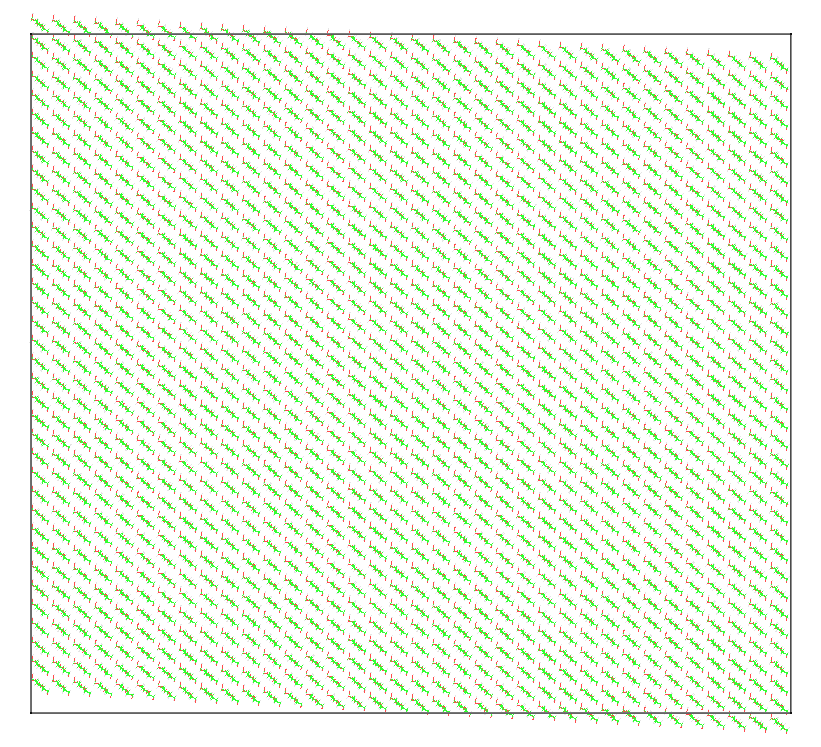
\includegraphics[width=0.12\textwidth]{cellulose_simulation_nanocrystal_different_size_i/model_1296.png}
        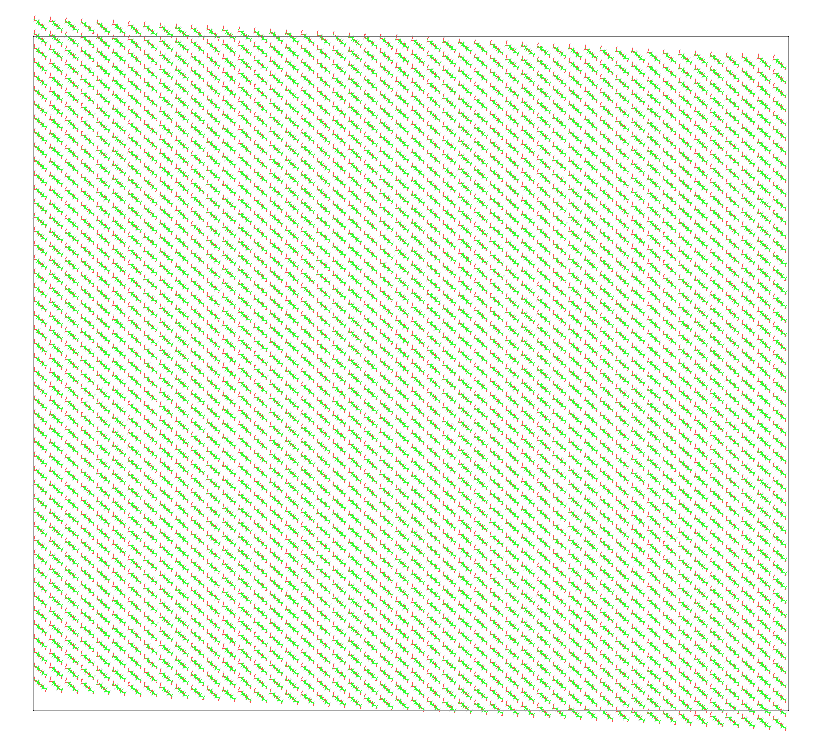
\includegraphics[width=0.12\textwidth]{cellulose_simulation_nanocrystal_different_size_i/model_2304.png}
        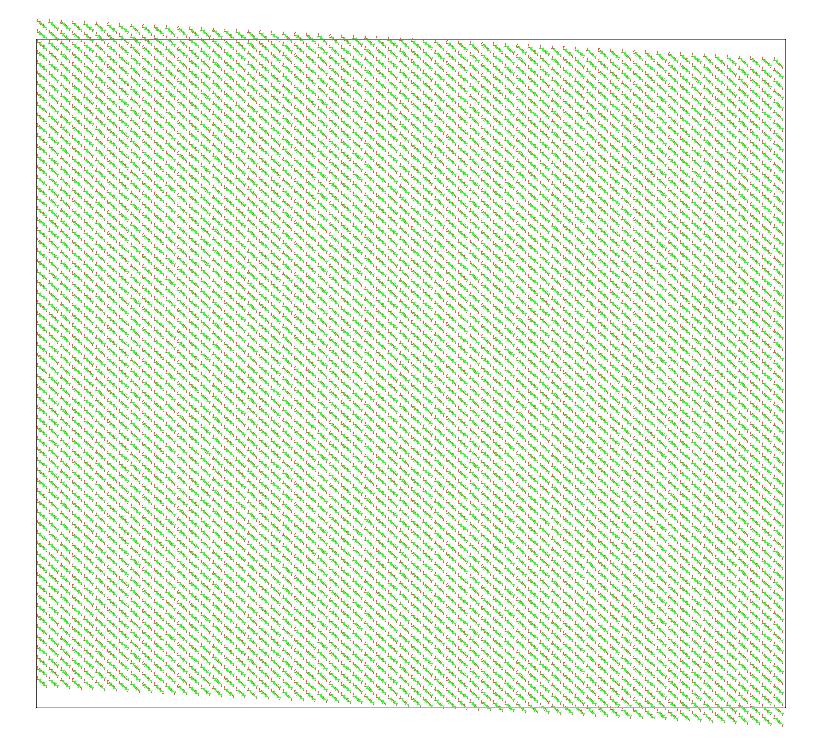
\includegraphics[width=0.12\textwidth]{cellulose_simulation_nanocrystal_different_size_i/model_4096.png}
        \subcaption{}
    \end{subfigure}
    \\
    \begin{subfigure}[b]{0.96\textwidth}
        \centering
        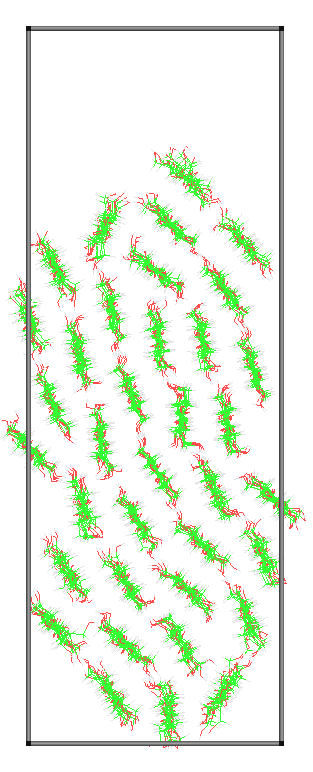
\includegraphics[width=0.12\textwidth]{cellulose_simulation_nanocrystal_different_size_i/fracture_36.png}
        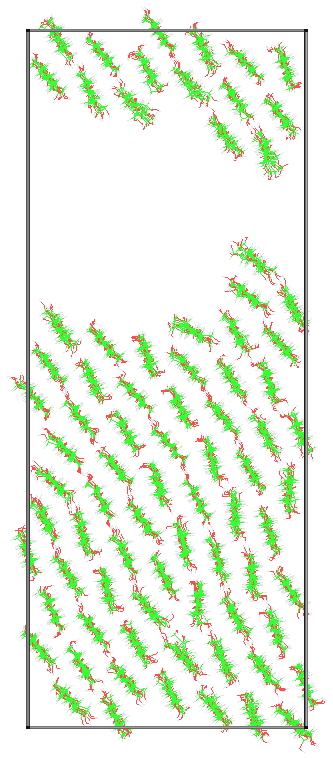
\includegraphics[width=0.12\textwidth]{cellulose_simulation_nanocrystal_different_size_i/fracture_81.png}
        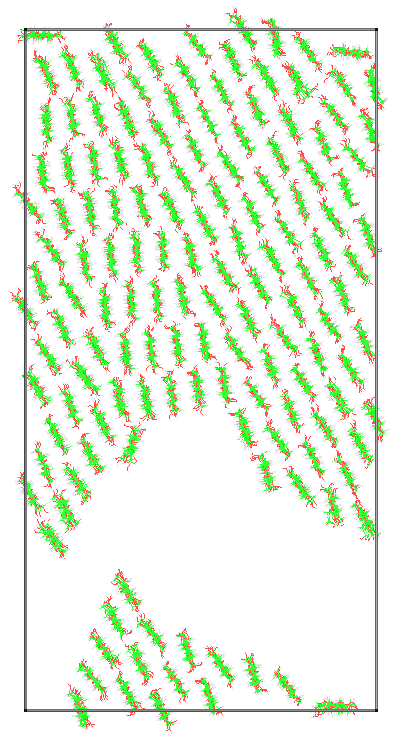
\includegraphics[width=0.12\textwidth]{cellulose_simulation_nanocrystal_different_size_i/fracture_144.png}
        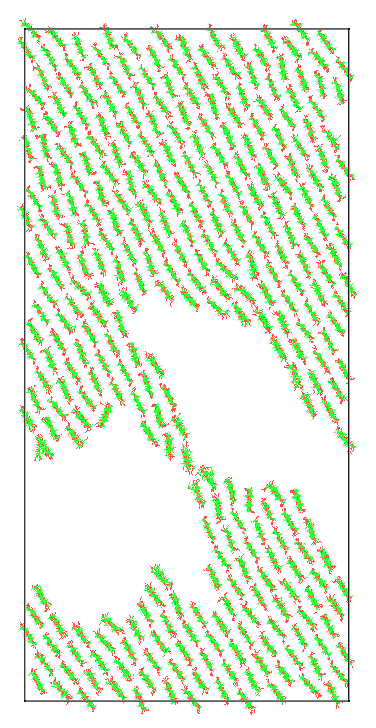
\includegraphics[width=0.12\textwidth]{cellulose_simulation_nanocrystal_different_size_i/fracture_324.png}
        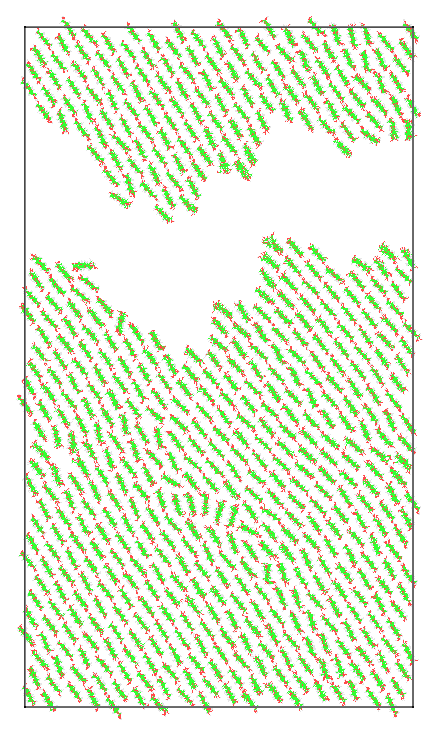
\includegraphics[width=0.12\textwidth]{cellulose_simulation_nanocrystal_different_size_i/fracture_576.png}
        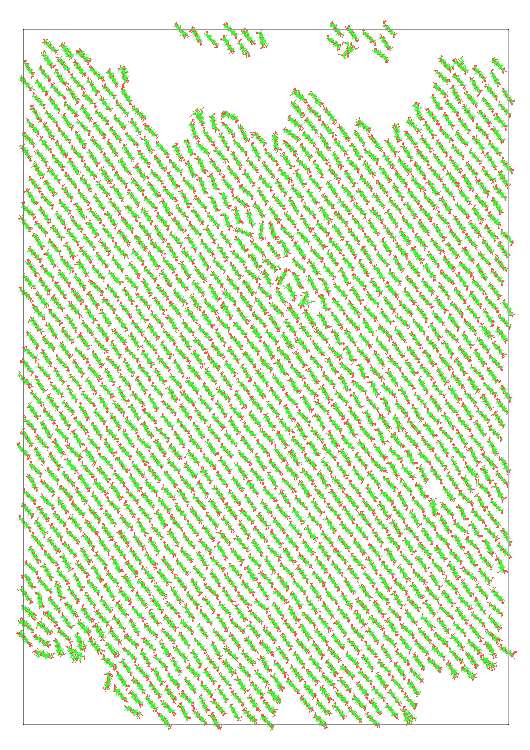
\includegraphics[width=0.12\textwidth]{cellulose_simulation_nanocrystal_different_size_i/fracture_1296.png}
        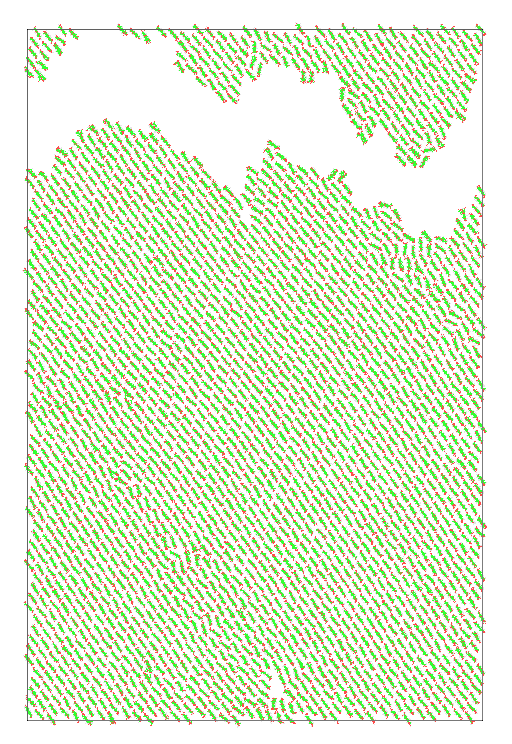
\includegraphics[width=0.12\textwidth]{cellulose_simulation_nanocrystal_different_size_i/fracture_2304.png}
        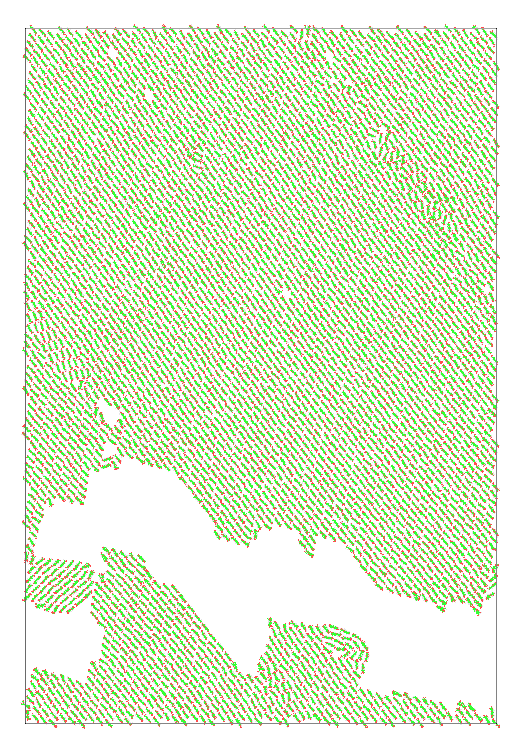
\includegraphics[width=0.12\textwidth]{cellulose_simulation_nanocrystal_different_size_i/fracture_4096.png}
        \subcaption{}
    \end{subfigure}
    \\
    \begin{subfigure}[b]{0.96\textwidth}
        \centering
        \begin{minipage}[b]{0.32\textwidth}
            \centering
            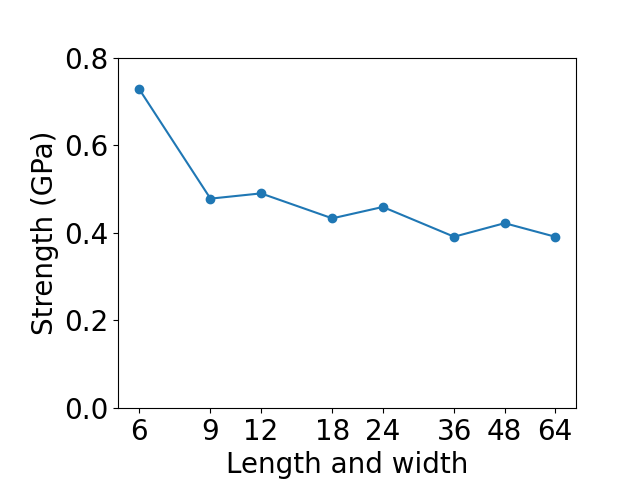
\includegraphics[width=0.96\textwidth]{cellulose_simulation_nanocrystal_different_size_i/stretch_strength_with_size.png}
        \end{minipage}
        \begin{minipage}[b]{0.32\textwidth}
            \centering
            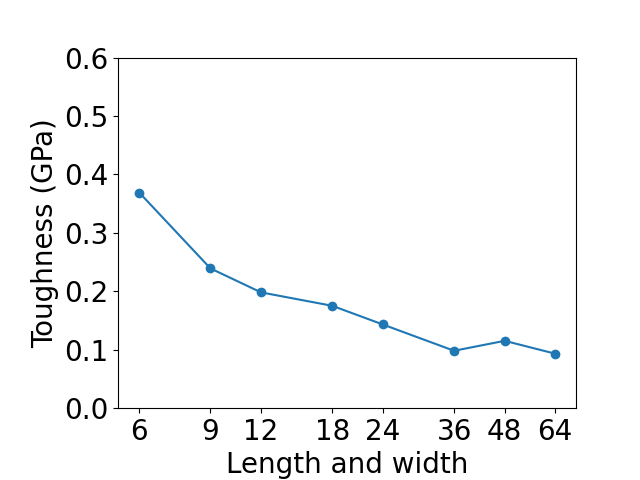
\includegraphics[width=0.96\textwidth]{cellulose_simulation_nanocrystal_different_size_i/stretch_toughness_with_size.png}
        \end{minipage}
        \begin{minipage}[b]{0.32\textwidth}
            \centering
            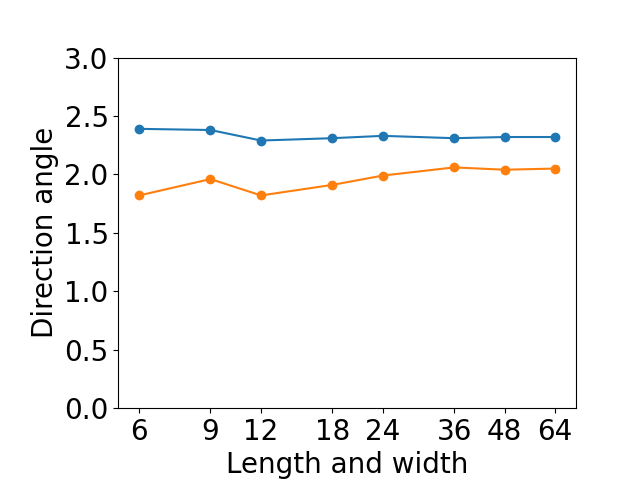
\includegraphics[width=0.96\textwidth]{cellulose_simulation_nanocrystal_different_size_i/stretch_direction_angle_with_size.png}
        \end{minipage}
        \subcaption{}
    \end{subfigure}
    \captionsetup{font=scriptsize}
    \caption{
    Models, fractures and performances of cellulose nanocrystals Type I with size.
    (a) Models of different sizes.
    The models considered here are cellulose nanocrystals Type I with the same number of rows and columns, such as 6$\times$6 and 12$\times$12.
    Specifically, the considered width or length were 6, 9, 12, 18, 24, 36, and 64.
    (b) Fractures of different sizes.
    From the perspective of fracture strain, it can be directly observed that ductility tended to decrease as the nanocrystal size increased.
    (c) Strength, toughness and direction angle with size.
    As the size increased, strength, toughness, and direction angle showed a decreasing tendency.
    }
    \label{fig:cellulose_nanocrystal_size_dependency}
\end{figure}

Robert Sinko et al. used RMSF (Root Mean Square Fluctuation) to explain the variation of mechanical properties with size for cellulose nanocrystals Type I.
Here, we use the delta potential energy density to explain the mechanical properties size dependency, as shown in Figure \ref{fig:cellulose_nanocrystal_delta_energy_density_with_size}.
The delta potential energy density was defined as the ratio of delta value of potential energy and the volume of the nanocrystal before stretching, or the amount of delta potential energy per unit volume.
As the size of nanocrystal increased, the absolute value of delta potential energy density during the stretch tended to decrease,  particularly for the Van der Waals interaction resisting stretch.
The special fracture behavior of the slant model of cellulose nanocrystals Type I is a local deformation morphology of frictional sliding between layers.
And the volume and overall potential energy increases approximately at the second power of length, but the potential energy of the interfaces of the friction sliding increased at lower order power of length, approximately linearly.
Consequently, the absolute value of delta potential energy per unit volume during the stretch gradually decreased as the model size increased, and the corresponding mechanical properties also decreased at a decaying rate.

\begin{figure}[htbp]
    \centering
    \begin{subfigure}[b]{0.48\textwidth}
        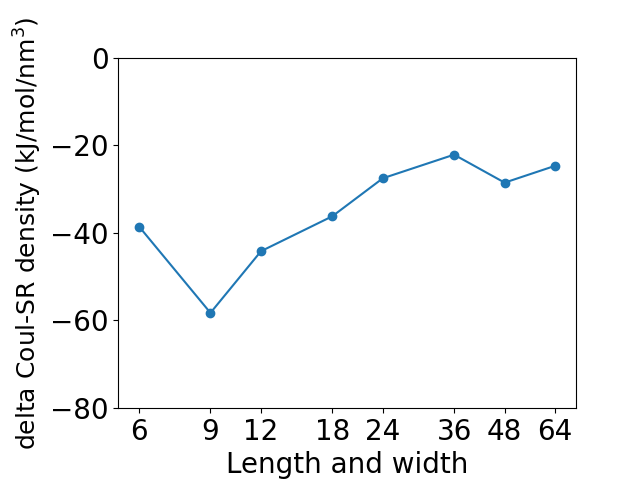
\includegraphics[width=0.96\textwidth]{cellulose_simulation_nanocrystal_different_size_i/stretch_delta_coul_sr_energy_density_with_size.png}
        \subcaption{}
    \end{subfigure}
    \begin{subfigure}[b]{0.48\textwidth}
        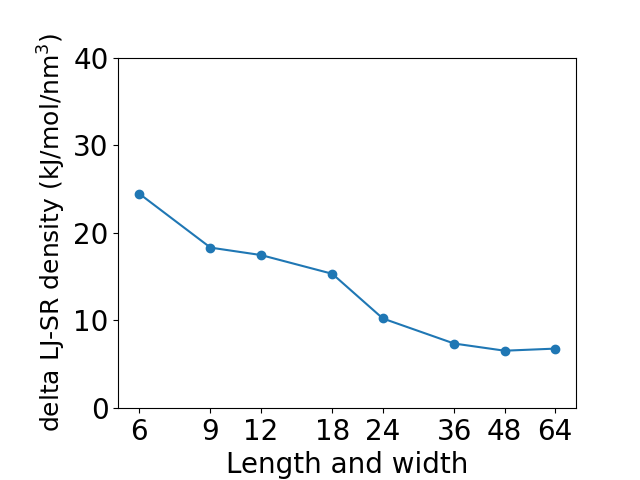
\includegraphics[width=0.96\textwidth]{cellulose_simulation_nanocrystal_different_size_i/stretch_delta_lj_sr_energy_density_with_size.png}
        \subcaption{}
    \end{subfigure}
    \captionsetup{font=scriptsize}
    \caption{
    Delta potential energy density of cellulose nanocrystals Type I with size.
    (a) Delta of Coulomb potential energy density and (b) Van der Waals potential energy density with size.
    The delta potential energy density was defined as the ratio of the delta potential energy during the stretch process relative to the crystal size before stretch, in other words, the delta potential energy per unit volume.
    As the size of the nanocrystal increased, the absolute value of delta potential energy density during stretches gradually decreased, particularly for the van der Waals interaction resisting tension.
    From the perspective of structure, larger nanocrystals have a stronger ability to maintain themselves.
    Even though friction-slip was observed in all the models, in larger nanocrystals, the parts away from the frictional sliding interface can maintain a structure similar to the crystal.
    The structural changes are not that significant compared to that in the smallest 6$\times$6 model.
    Inferring from the delta potential energy density, the damage to cellulose nanocrystals is a localized interaction at the frictional sliding interface, therefore the delta potential energy density does not grow linearly with the crystal volume.
    The volumes of the nanocrystal grows with the second power of the length, while the delta potential energy of the friction-slip interface increased with a lower power.
    Therefore, the delta potential energy density and mechanical performance of cellulose nanocrystals weakened as the size increased.
    }
    \label{fig:cellulose_nanocrystal_delta_energy_density_with_size}
\end{figure}

\subsubsection{Toughening mechanism inspired by anisotropy and size dependency}\indent

Considering the size dependency of the mechanical performance of cellulose nanocrystals, we propose to consider the transverse arrangement of unit blocks to tune the overall mechanical performance of the structure.
A structure formed by smaller unit blocks in a certain arrangement pattern may have better mechanical performance than a single cellulose nanocrystal of the same size.
Inspired by the twin structure, we proposed a symmetric pattern and a cross pattern (the cross pattern is a further symmetric pattern to the symmetric patter, Figure \ref{fig:cellulose_nanocrystal_transverse_arrangement_fractures}).
These two pattern still have differences in structure and mechanical properties in the horizontal and vertical directions;
and models composed of different size unit nanocrystal blocks were constructed to examine the size dependency.
The specific unit blocks sizes considered include 6$\times$6, 9$\times$9, and 12$\times$12, and 4 units were arranged to form the final structure.
The models and fractures of the arranged structure is shown in Figure \ref{fig:cellulose_nanocrystal_transverse_arrangement_fractures}.

The mechanical properties of the slant model of Type II cellulose nanocrystals significantly depend on crystal structure periodicity (this will be further explained in the simulation containing solvents in the following sections).
Otherwise, it is difficult to restructure and exhibit good toughness, and only the symmetric pattern under vertical stretches could exhibit higher toughness than crystal structure.
The size dependency and transverse toughening simulation data are shown in Figure \ref{fig:cellulose_nanocrystal_ii_size_dependency} and Figure \ref{fig:cellulose_nanocrystal_ii_delta_energy_density_with_size} for reference.

Simulation results show that symmetric and cross patterns can improve the ductility and toughness of the structure, influenced by the size of its unit blocks at the meantime.
In symmetric and cross patterns, the friction sliding was hindered, and local rotation replaced it as the dominant deformation phenomenon.
Structures subjected to horizontal stretches were rotated counter clockwise for the easiness of comparisons.
The internal interfaces of symmetric and cross patterns unit blocks are weaker in the horizontal direction, correspondingly, the ductility and toughness when subjected to  horizontal stretches was also worse, particularly for the symmetric pattern.
In summary, the cross pattern had better ductility and toughness when subjected to both vertical and horizontal stretches, and the symmetric pattern preferred vertical loads.
The ductility of the arranged structure is also significantly related to the size of unit blocks, the structure formed by 6$\times$6 constituent units has better ductility.
Specific quantitative performance comparisons of arrangement pattern and crystal structure of the same size are given in Figure \ref{fig:cellulose_nanocrystal_transverse_arrangement_performance_with_patterns}.

To reduce the influence of manual settings on the simulation results, arranged structures composed of 16 unit blocks were constructed and tested (Figure \ref{fig:cellulose_nanocrystal_more_transverse_arrangement_fractures} and Figure \ref{fig:cellulose_nanocrystal_ii_more_transverse_arrangement_fractures}).
With more unit blocks of arrangements, the local rotation still replaced the hindered friction-slip.
Because the interfacial interaction strength between unit blocks is weak in cross patterns, when the number of unit block increased, the arranged structure was more significantly affected by the size of the unit crystals and still outperform if using 6$\times$6 unit blocks.
Considering the quantitative performances and fracture behaviors of the two patterns, arranging small unit blocks in these patterns rather than forming a single larger nanocrystal, is an effective toughening mechanism.

\begin{figure}[htbp]
    \centering
    \scriptsize
    \begin{subfigure}[b]{0.96\textwidth}
        \centering
        \begin{minipage}[b]{0.24\textwidth}
            \centering
            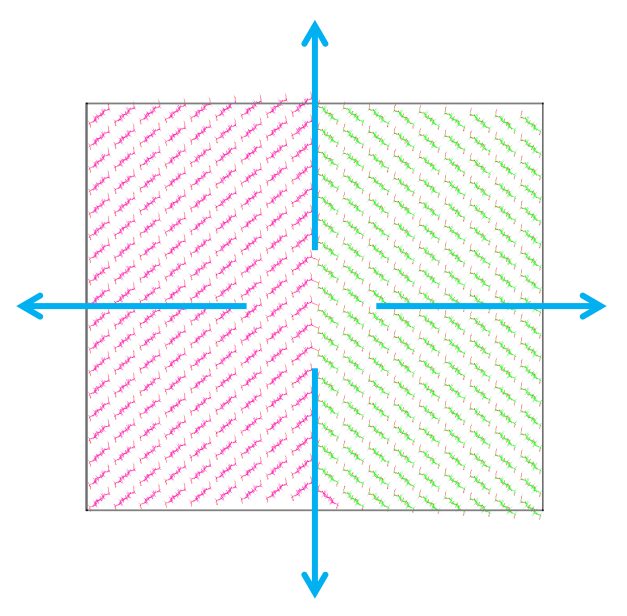
\includegraphics[width=0.96\textwidth]{cellulose_simulation_transverse_arrangement_i/transverse_arrangement_pattern_symmetric.png}
            \\
            Symmetric
        \end{minipage}
        \begin{minipage}[b]{0.24\textwidth}
            \centering
            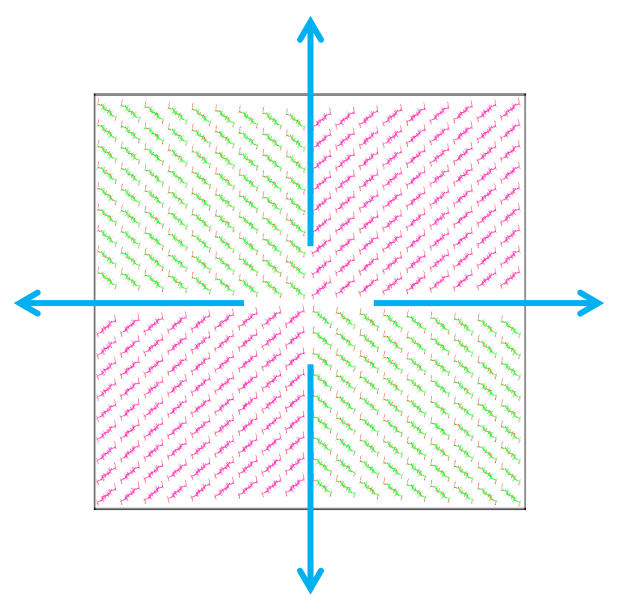
\includegraphics[width=0.96\textwidth]{cellulose_simulation_transverse_arrangement_i/transverse_arrangement_pattern_cross.png}
            \\
            Cross
        \end{minipage}
        \subcaption{}
    \end{subfigure}
    \\
    \begin{subfigure}[b]{0.96\textwidth}
        \centering
        \begin{minipage}[b]{0.36\textwidth}
            \centering
            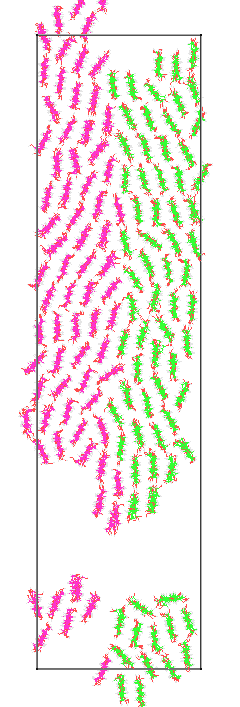
\includegraphics[width=0.24\textwidth]{cellulose_simulation_transverse_arrangement_i/fracture_symmetric_36x4.png}
            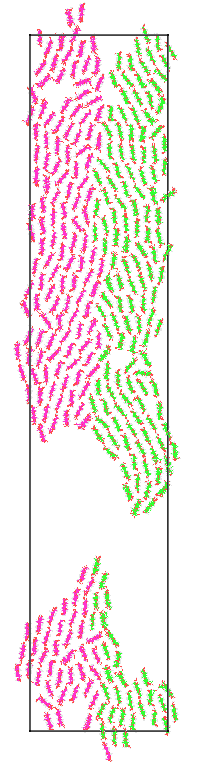
\includegraphics[width=0.24\textwidth]{cellulose_simulation_transverse_arrangement_i/fracture_symmetric_81x4.png}
            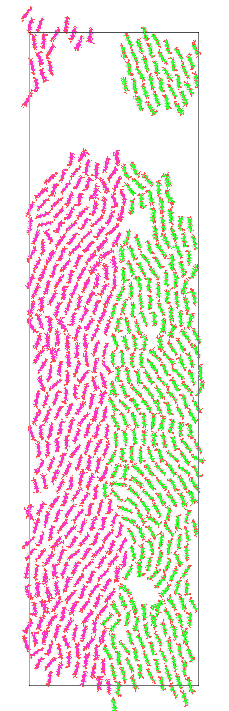
\includegraphics[width=0.24\textwidth]{cellulose_simulation_transverse_arrangement_i/fracture_symmetric_144x4.png}
            \\
            Symmetric
        \end{minipage}
        \hspace{0.12\textwidth}
        \begin{minipage}[b]{0.36\textwidth}
            \centering
            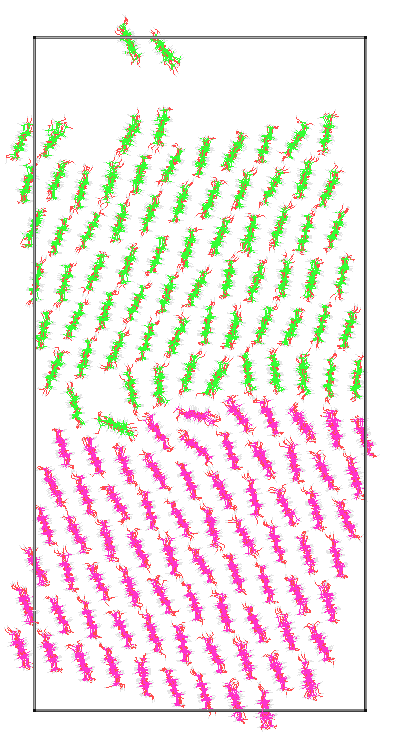
\includegraphics[width=0.24\textwidth]{cellulose_simulation_transverse_arrangement_i/fracture_symmetric_horizontal_36x4.png}
            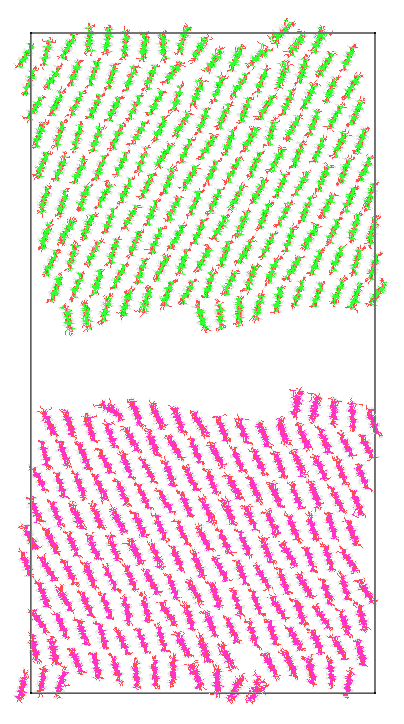
\includegraphics[width=0.24\textwidth]{cellulose_simulation_transverse_arrangement_i/fracture_symmetric_horizontal_81x4.png}
            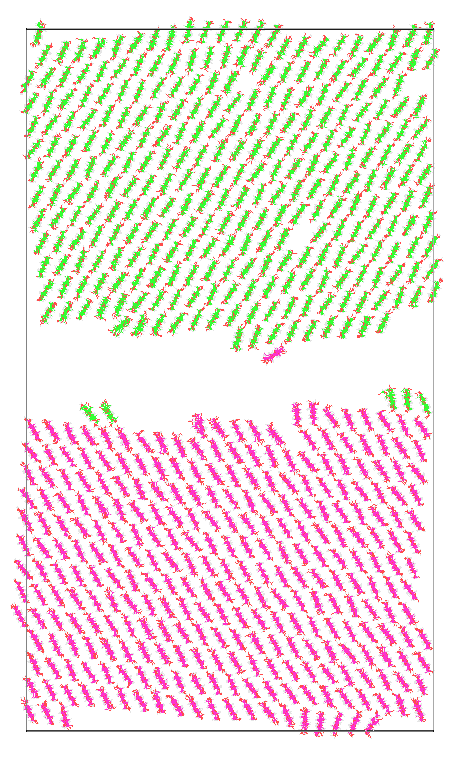
\includegraphics[width=0.24\textwidth]{cellulose_simulation_transverse_arrangement_i/fracture_symmetric_horizontal_144x4.png}
            \\
            Symmetric Horizontal
        \end{minipage}
        \subcaption{}
    \end{subfigure}
    \\
    \begin{subfigure}[b]{0.96\textwidth}
        \centering
        \begin{minipage}[b]{0.36\textwidth}
            \centering
            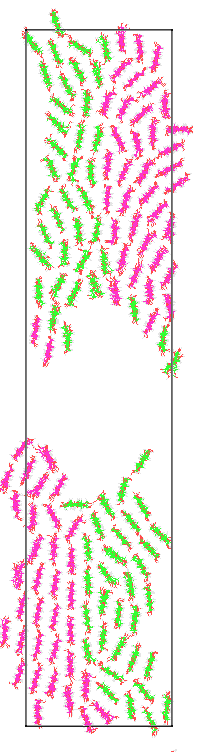
\includegraphics[width=0.24\textwidth]{cellulose_simulation_transverse_arrangement_i/fracture_cross_36x4.png}
            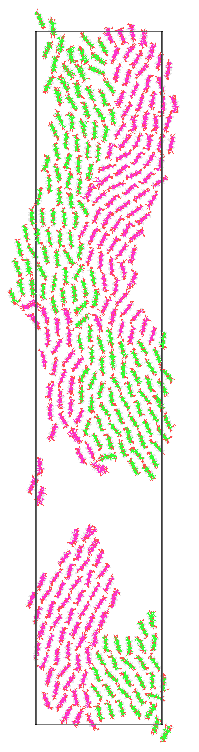
\includegraphics[width=0.24\textwidth]{cellulose_simulation_transverse_arrangement_i/fracture_cross_81x4.png}
            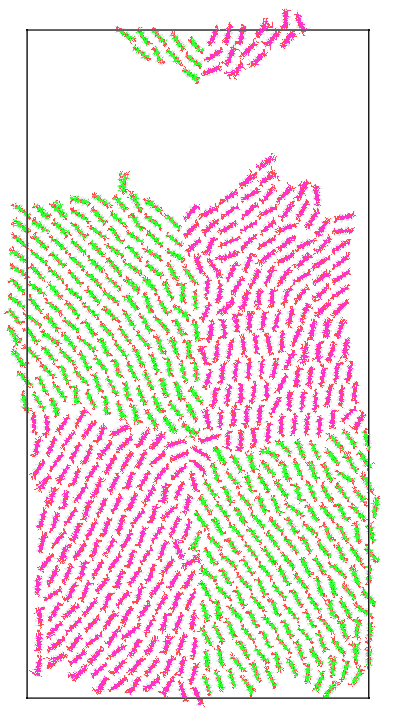
\includegraphics[width=0.24\textwidth]{cellulose_simulation_transverse_arrangement_i/fracture_cross_144x4.png}
            \\
            Cross
        \end{minipage}
        \hspace{0.12\textwidth}
        \begin{minipage}[b]{0.36\textwidth}
            \centering
            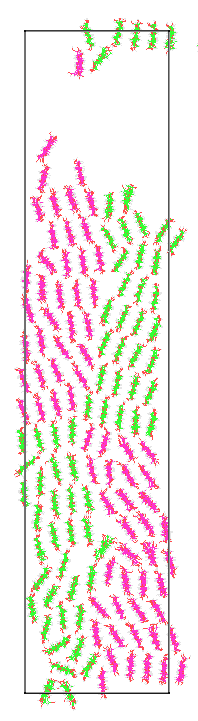
\includegraphics[width=0.24\textwidth]{cellulose_simulation_transverse_arrangement_i/fracture_cross_horizontal_36x4.png}
            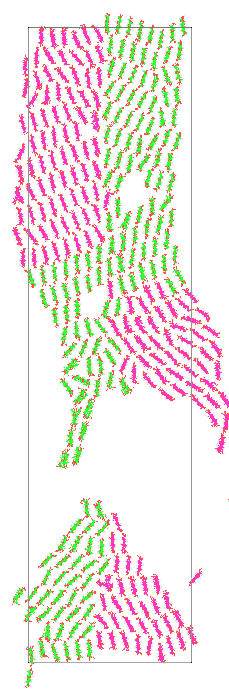
\includegraphics[width=0.24\textwidth]{cellulose_simulation_transverse_arrangement_i/fracture_cross_horizontal_81x4.png}
            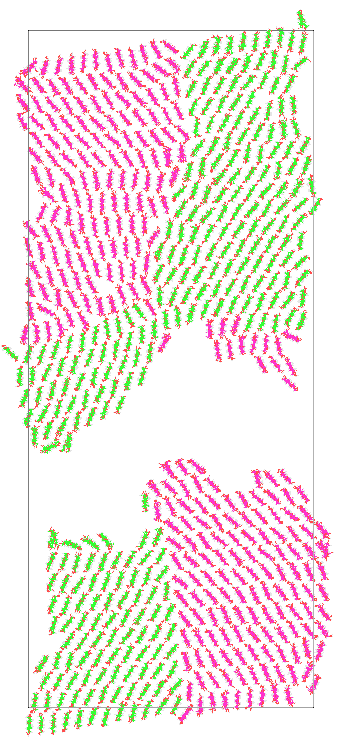
\includegraphics[width=0.24\textwidth]{cellulose_simulation_transverse_arrangement_i/fracture_cross_horizontal_144x4.png}
            \\
            Cross Horizontal
        \end{minipage}
        \subcaption{}
    \end{subfigure}
    \captionsetup{font=scriptsize}
    \caption{
    Transverse arrangement patterns and corresponding fractures of cellulose nanocrystals Type I.
    (a) Two transverse arrangement patterns: symmetric and cross.
    The symmetric pattern is inspired by twin structures, and the cross pattern is a further symmetrical arrangement.
    The performance of the two arrangement modes differs in the vertical and horizontal directions, and models were stretched at both the directions.
    The structures stretched under horizontal loads were rotated counter clockwise, including models of different unit block sizes (6$\times$6, 9$\times$9, and 12$\times$12 rows and columns, and one model were composed of 4 of unit blocks).
    (b) Fractures of symmetrical arrangements under vertical and horizontal stretches.
    Symmetrical arrangements exhibited good toughness and ductility under vertical loading, but were weak when subjected to horizontal loading.
    (c) Fractures of cross arrangements under vertical and horizontal stretches.
    Cross arrangements exhibited good toughness and ductility under both vertical and horizontal loading, serving as an effective toughening mechanism.
    In both symmetrical and cross arrangements, the frictional sliding of each unit was hindered, leading localized rotation to become the dominant deformation mechanism, which resulted in improved toughness and ductility.
    On the other hand, these arrangements were also affected by the size-dependency of units.
    The structures composed of smaller units exhibited better toughness and ductility.
    }
    \label{fig:cellulose_nanocrystal_transverse_arrangement_fractures}
\end{figure}

Figure \ref{fig:cellulose_nanocrystal_transverse_arrangement_performance_with_patterns} provides quantitative data on the influences of arrangement pattern, loading direction, and unit block size on strength and toughness.
These data confirmed the previous conclusions based on morphological results.
Compared to nanocrystal models of the same size, the strength of symmetric and cross patterns decreased, but the toughness significantly improved, particularly in the case of small unit blocks.
With further technological development and requirements of material design, the transverse arrangement of cellulose nanocrystals.

\begin{figure}[htbp]
    \centering
    \begin{subfigure}[b]{0.96\textwidth}
        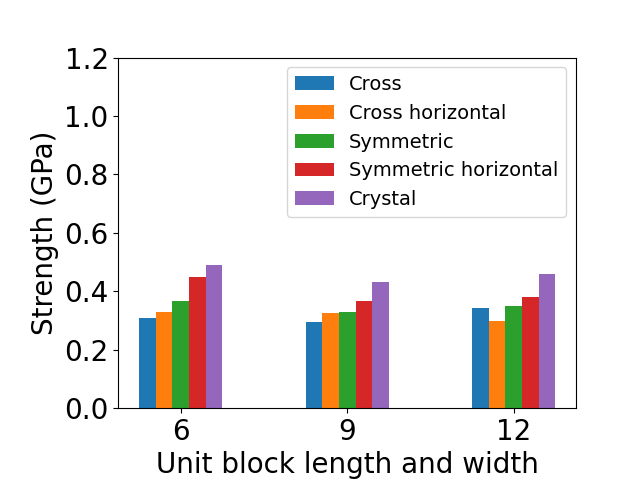
\includegraphics[width=0.48\textwidth]{cellulose_simulation_transverse_arrangement_i/stretch_strength_with_pattern.png}
        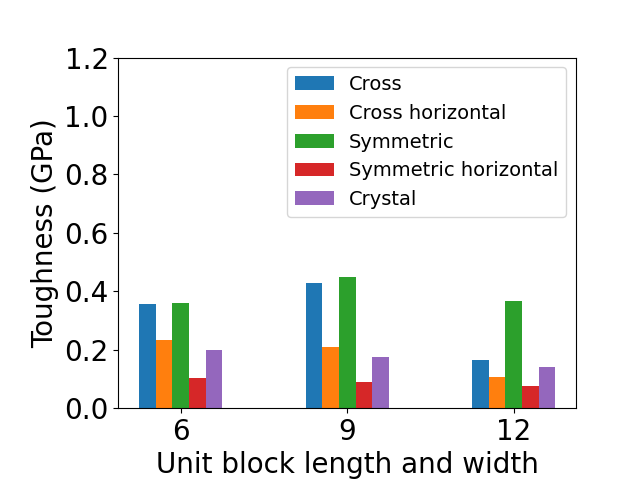
\includegraphics[width=0.48\textwidth]{cellulose_simulation_transverse_arrangement_i/stretch_toughness_with_pattern.png}
        \subcaption{}
    \end{subfigure}
    \\
    \begin{subfigure}[b]{0.96\textwidth}
        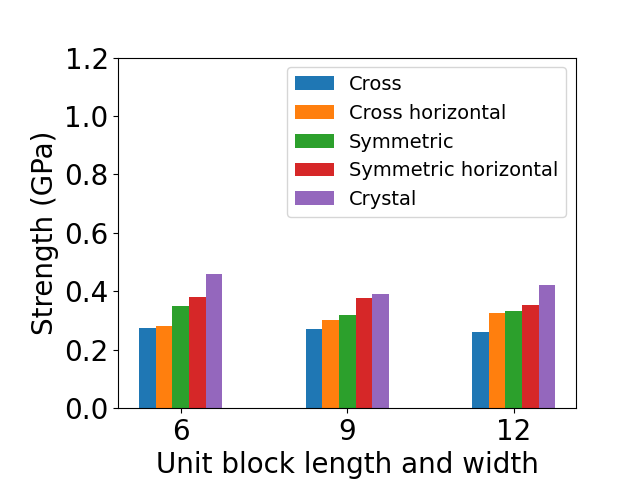
\includegraphics[width=0.48\textwidth]{cellulose_simulation_transverse_arrangement_i/stretch_strength_with_pattern_larger.png}
        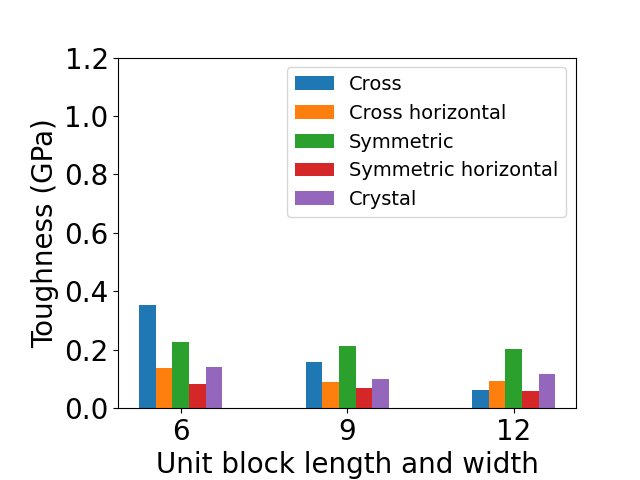
\includegraphics[width=0.48\textwidth]{cellulose_simulation_transverse_arrangement_i/stretch_toughness_with_pattern_larger.png}
        \subcaption{}
    \end{subfigure}
    \captionsetup{font=scriptsize}
    \caption{
    Mechanical performances of transverse arrangement patterns of cellulose nanocrystal Type I.
    (a) Strength and toughness of transverse patterns.
    (b) Strength and toughness of transverse patterns with more unit blocks.
    By comparing with crystal models of the same sizes, it is clear that both symmetric and cross patterns can improved the ductility and toughness significantly with a little sacrifice on strength.
    These toughening mechanisms of transverse patterns and dependency of small unit block size were further represented by models composed of 16 unit blocks.
    }
    \label{fig:cellulose_nanocrystal_transverse_arrangement_performance_with_patterns}
\end{figure}

\subsubsection{Mechanical properties of cellulose nanocrystals when surrounded by solvents on both sides}\indent

Under natural conditions (such as cellulose crystals in plants) and non-natural conditions (such as advanced materials like composites prepared artificially), solvents represented by water often coexist with cellulose nanocrystals, as described in the ``Introduction''.
Analyzing the influence of the solvent environment is very important for understanding cellulose nanocrystals in real environments and can also assist in the development of cellulose materials.
Referring to relevant literature, eight solvents were selected: DMF (N,N-Dimethylformamide)\cite{bui2022synthesis}, DMSO (Dimethyl sulfoxide)\cite{dong2024preparation}, EDA (ethylenediamine)\cite{li2024mild}, ETA (ethanol)\cite{yang2025evaluating}, IPA (isopropanol)\cite{yeo2022robust}, MTA (methanol)\cite{przybylek2023use}, and SOL (water)\cite{etale2023cellulose}, alongside a NONE (solvent-free) control group.
Some abbreviations of solvents used here are non-standard.
In a solvent environment, both the cellulose nanocrystals themselves, and the interaction between cellulose and the solvent are important influencing factors.

When considering the mechanical properties of cellulose nanocrystals in the previous sections, the cellulose nanocrystals were simulated in a fully xyz periodic boundary conditions.
The emphasis of this section contains two parts: first, to consider the mechanical properties of cellulose nanocrystals under non-fully periodic boundary conditions; second, to consider the impact of solvents on the mechanical properties of cellulose nanocrystals.
The solvent surrounded model considered was defined as, where the overall model still maintained xyz periodic boundary conditions, but the left and right sides of the nanocrystal were non-continuous and surrounded by solvents.
In this surrounded model, cellulose nanocrystals were only periodic in the y and z directions.
The specific models and stretches are shown in Figure \ref{fig:cellulose_nanocrystal_with_solvent_around_fractures}.
The eight solvent condition models are arranged as the first row (DMF, DMSO, EDA, ETA) and second row (IPA, MTA, SOL, NONE), and the same vertical strain was applied to these models.
For the solvent-free control group, pressure control was performed in the yz directions only, while all other solvent groups were controlled in the xyz directions.

\begin{figure}[htbp]
    \centering
    \begin{subfigure}[b]{0.96\textwidth}
        \centering
        \begin{minipage}[b]{0.12\textwidth}
            \centering
            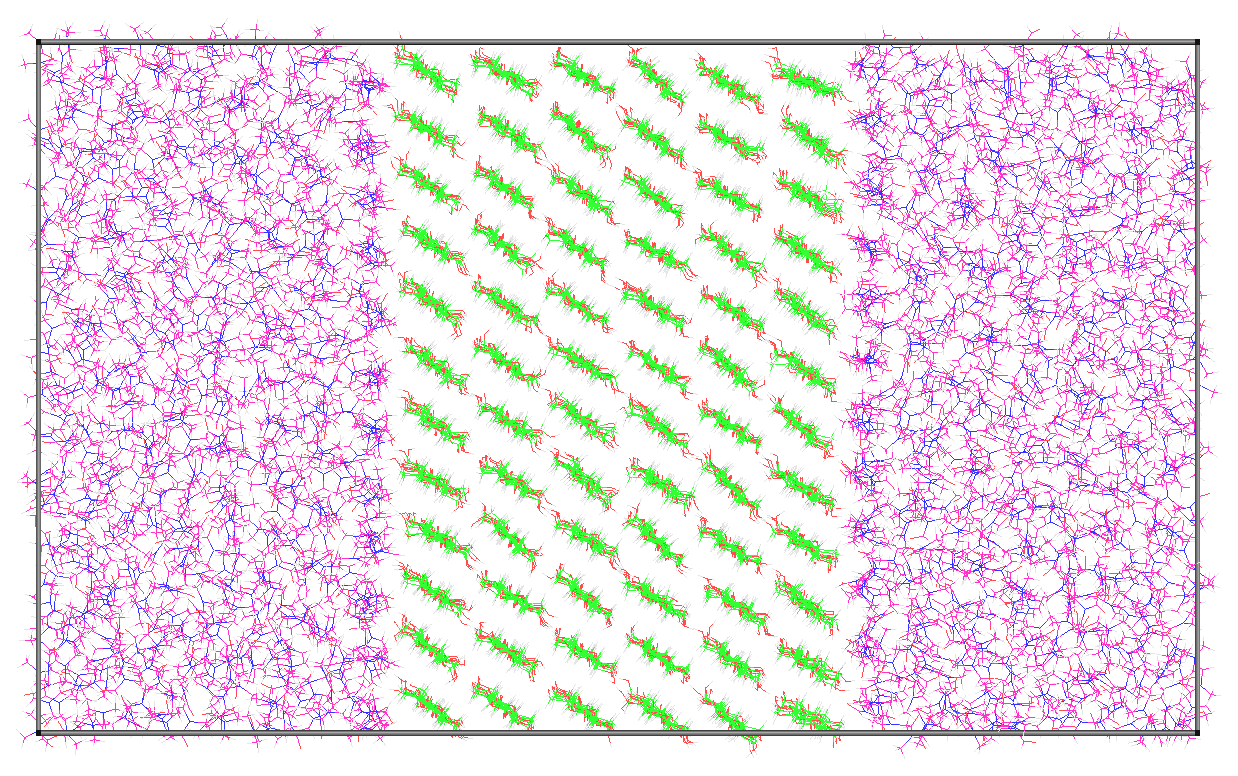
\includegraphics[height=0.57\textwidth]{cellulose_simulation_with_solvent_around_i/relaxation_with_dmf_around.png}
        \end{minipage}
        \begin{minipage}[b]{0.12\textwidth}
            \centering
            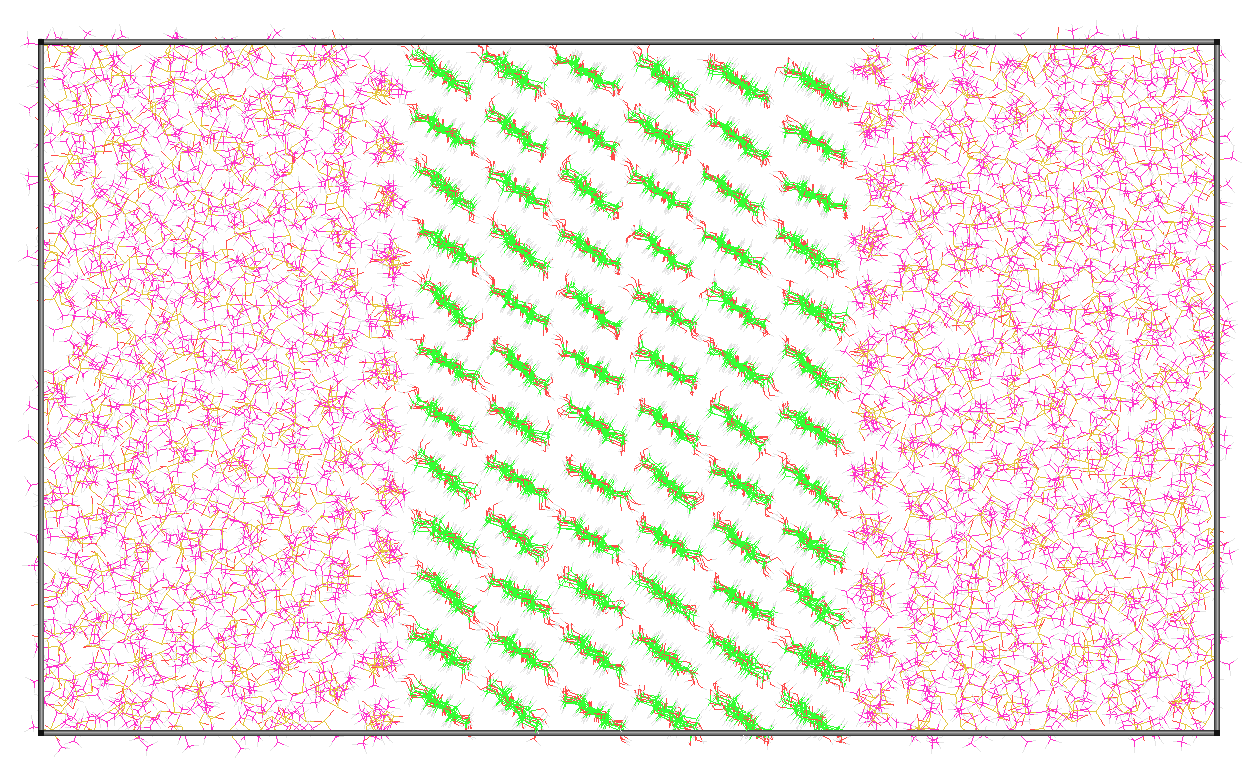
\includegraphics[height=0.57\textwidth]{cellulose_simulation_with_solvent_around_i/relaxation_with_dmso_around.png}
        \end{minipage}
        \begin{minipage}[b]{0.12\textwidth}
            \centering
            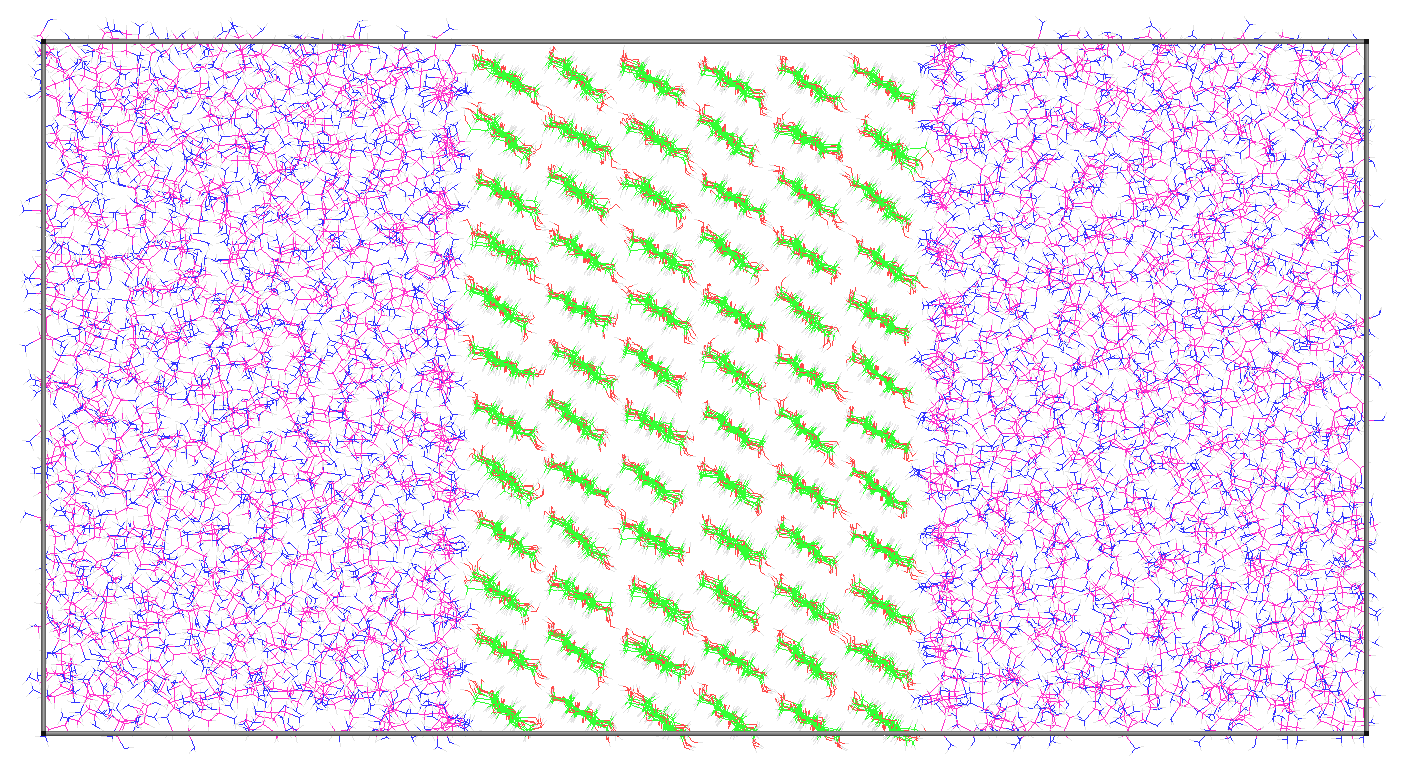
\includegraphics[height=0.57\textwidth]{cellulose_simulation_with_solvent_around_i/relaxation_with_eda_around.png}
        \end{minipage}
        \begin{minipage}[b]{0.12\textwidth}
            \centering
            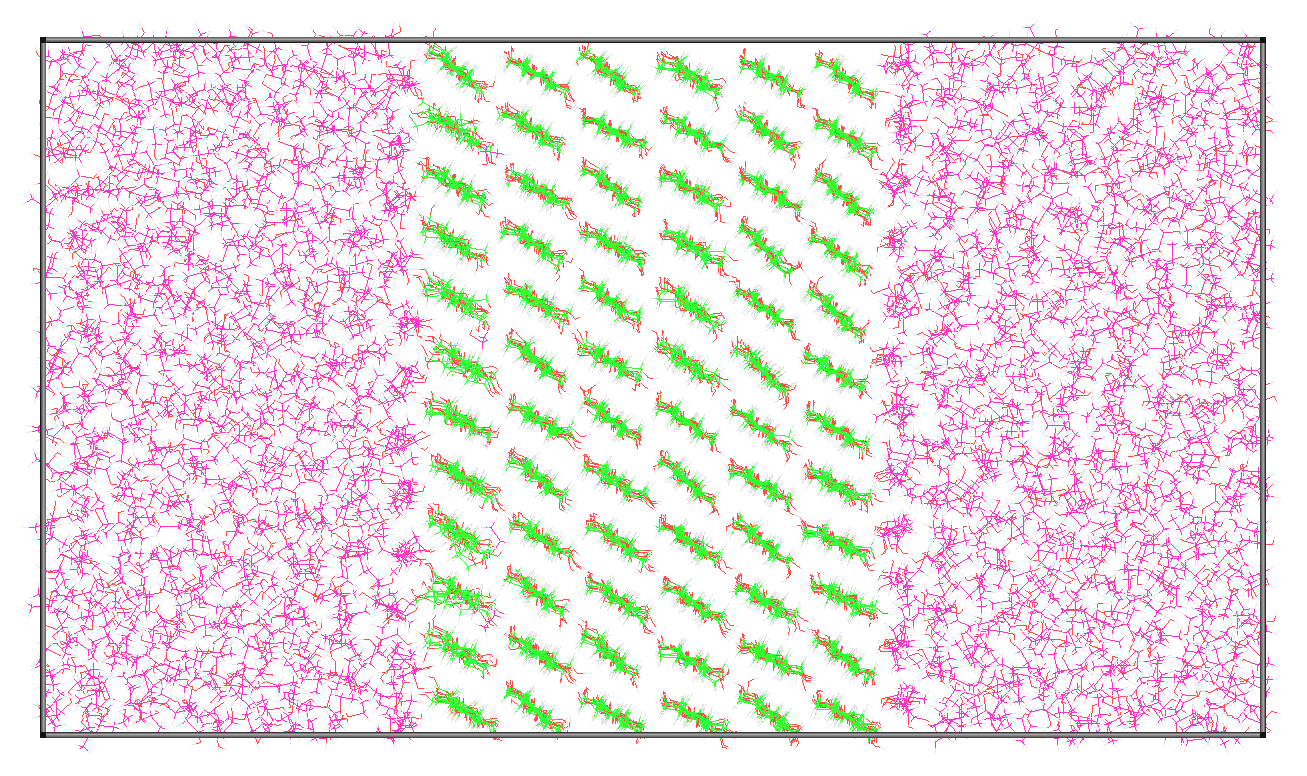
\includegraphics[height=0.57\textwidth]{cellulose_simulation_with_solvent_around_i/relaxation_with_eta_around.png}
        \end{minipage}
        \\
        \begin{minipage}[b]{0.12\textwidth}
            \centering
            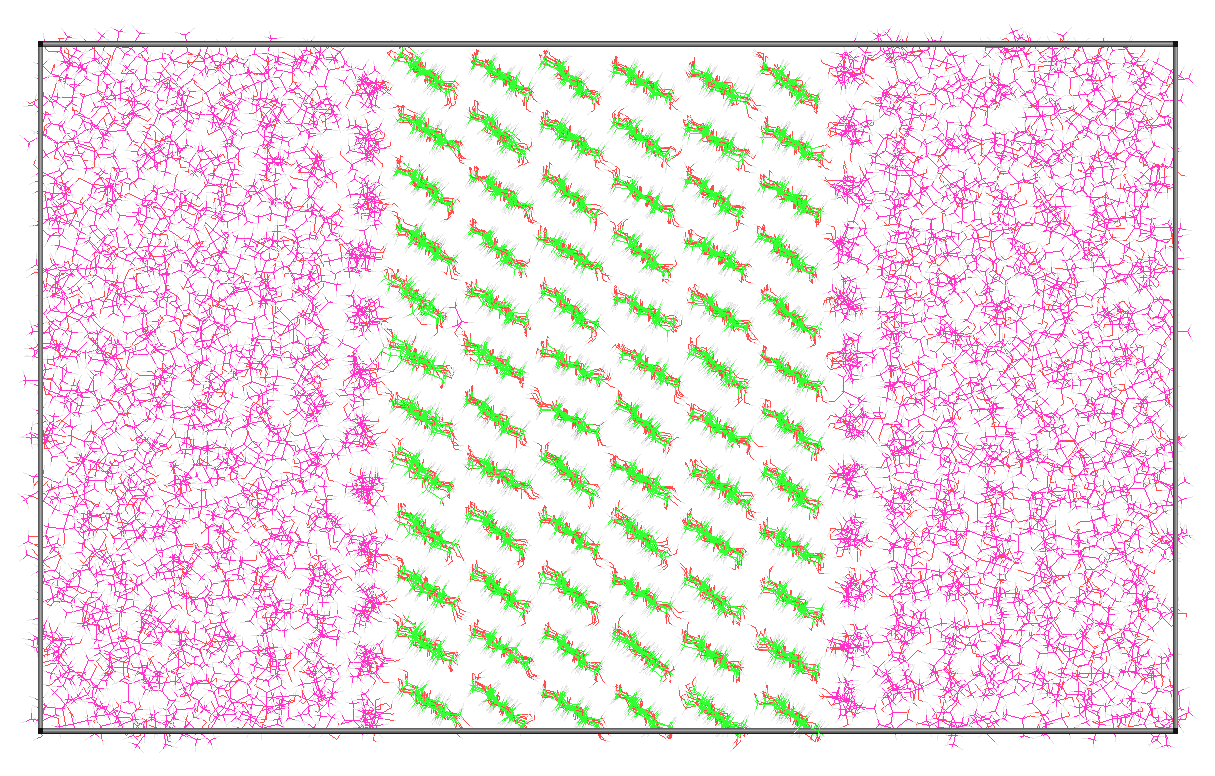
\includegraphics[height=0.57\textwidth]{cellulose_simulation_with_solvent_around_i/relaxation_with_ipa_around.png}
        \end{minipage}
        \begin{minipage}[b]{0.12\textwidth}
            \centering
            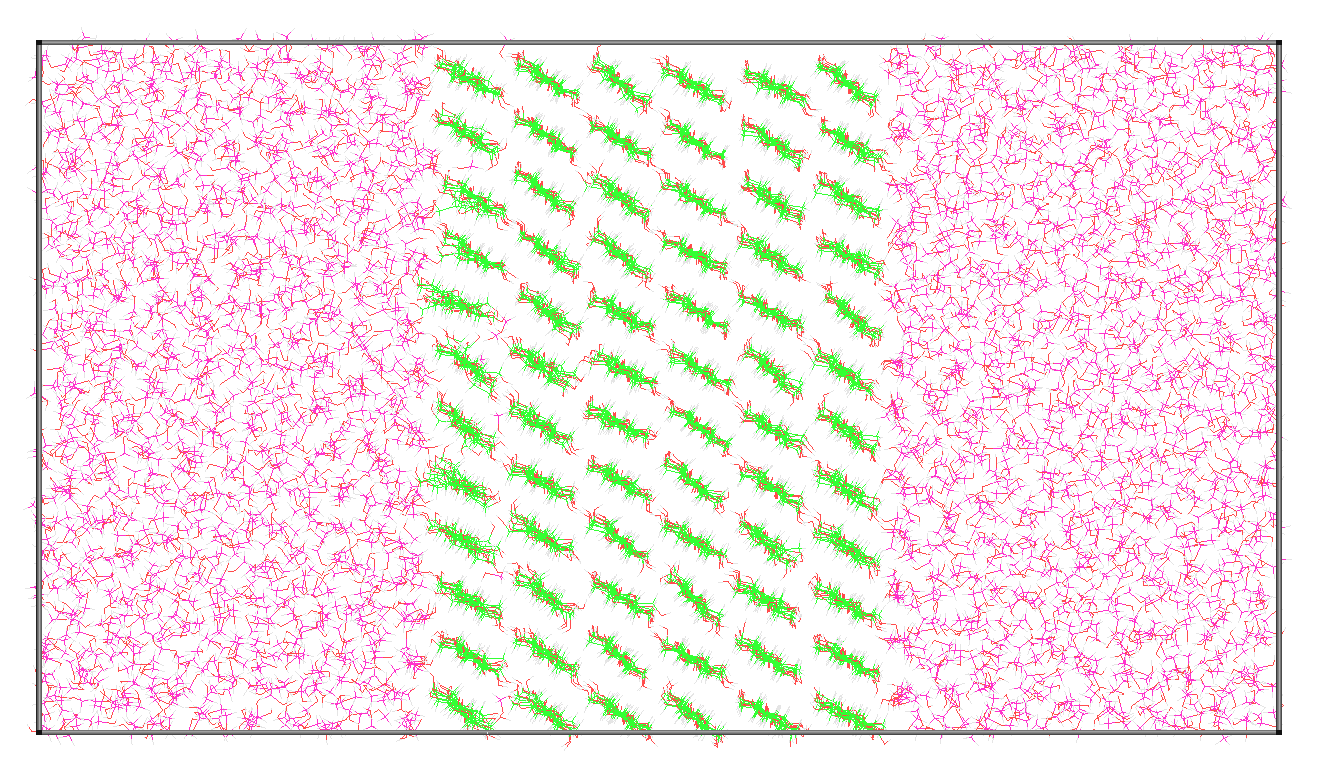
\includegraphics[height=0.57\textwidth]{cellulose_simulation_with_solvent_around_i/relaxation_with_mta_around.png}
        \end{minipage}
        \begin{minipage}[b]{0.12\textwidth}
            \centering
            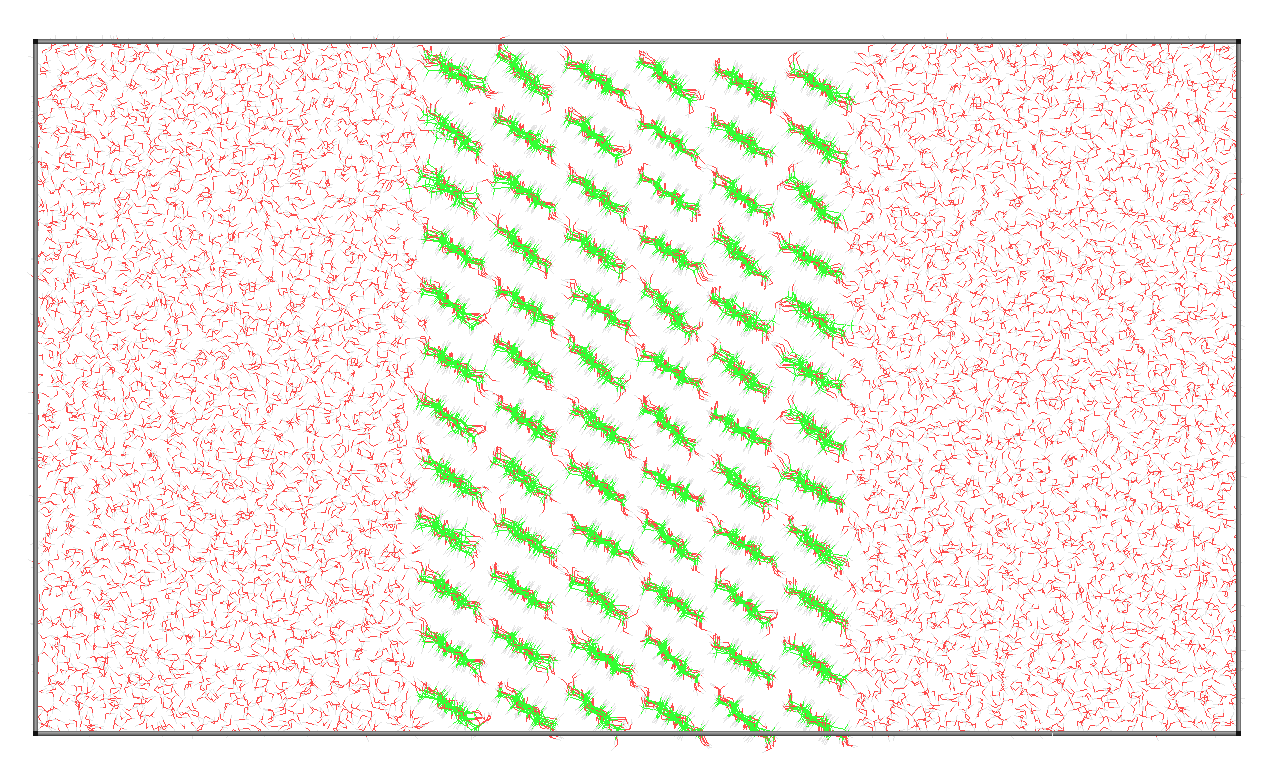
\includegraphics[height=0.57\textwidth]{cellulose_simulation_with_solvent_around_i/relaxation_with_sol_around.png}
        \end{minipage}
        \begin{minipage}[b]{0.12\textwidth}
            \centering
            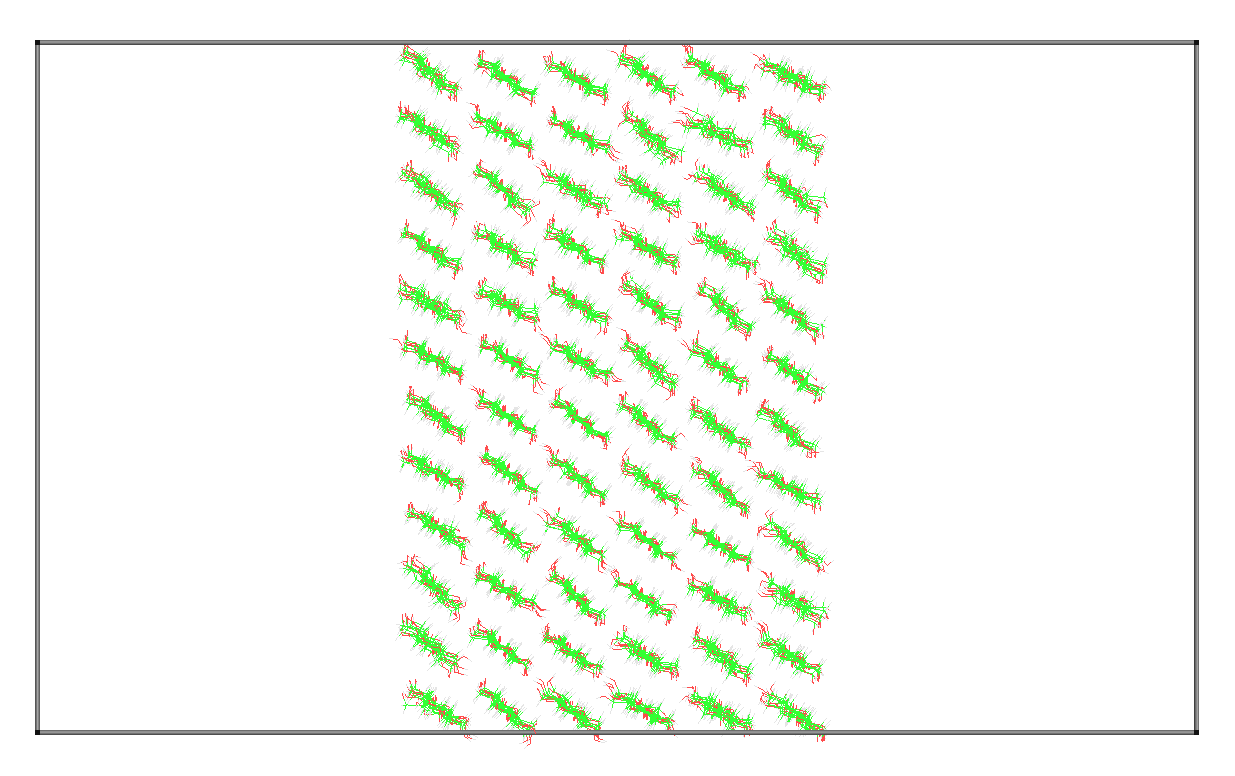
\includegraphics[height=0.57\textwidth]{cellulose_simulation_with_solvent_around_i/relaxation_with_none_around.png}
        \end{minipage}
        \subcaption{}
    \end{subfigure}
    \\
    \begin{subfigure}[b]{0.96\textwidth}
        \centering
        \begin{minipage}[b]{0.12\textwidth}
            \centering
            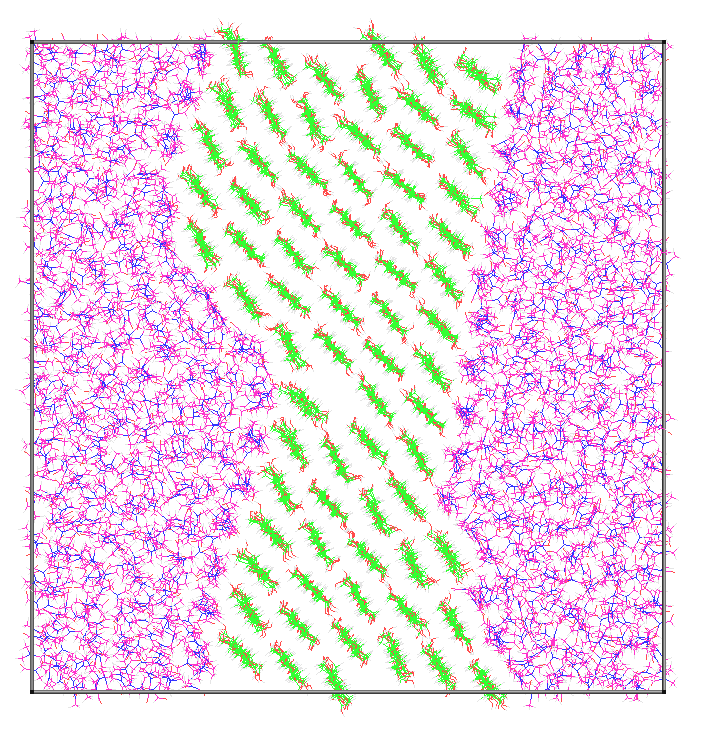
\includegraphics[height=0.75\textwidth]{cellulose_simulation_with_solvent_around_i/transition_with_dmf_around.png}
        \end{minipage}
        \begin{minipage}[b]{0.12\textwidth}
            \centering
            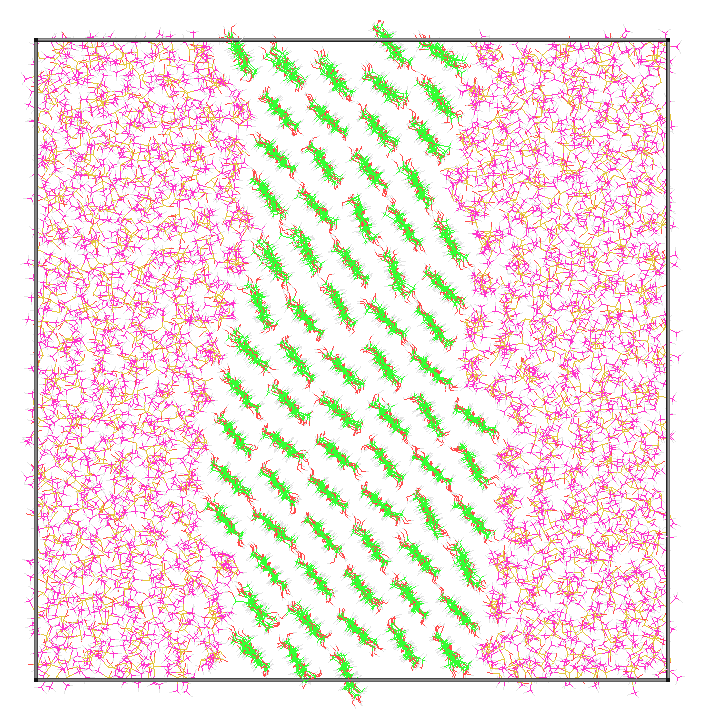
\includegraphics[height=0.75\textwidth]{cellulose_simulation_with_solvent_around_i/transition_with_dmso_around.png}
        \end{minipage}
        \begin{minipage}[b]{0.12\textwidth}
            \centering
            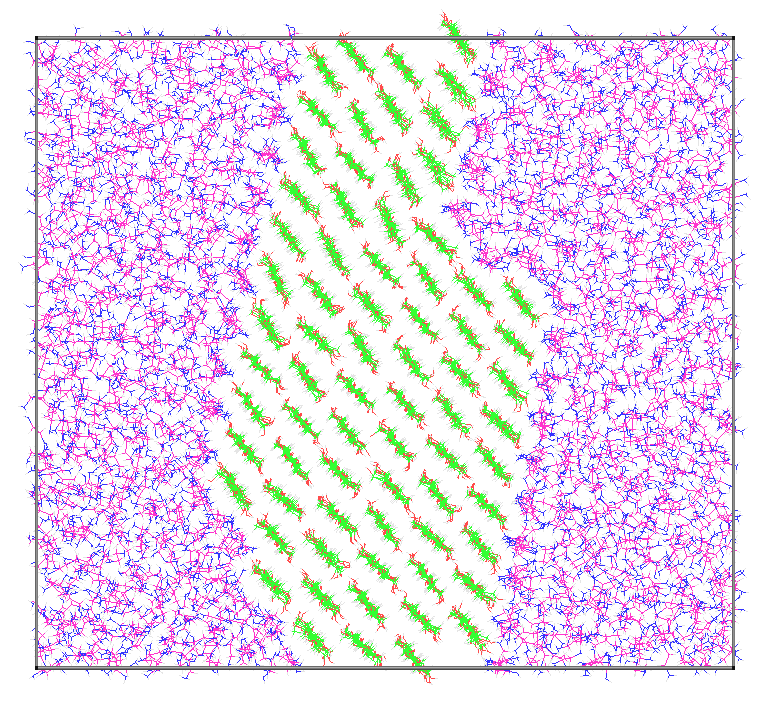
\includegraphics[height=0.75\textwidth]{cellulose_simulation_with_solvent_around_i/transition_with_eda_around.png}
        \end{minipage}
        \begin{minipage}[b]{0.12\textwidth}
            \centering
            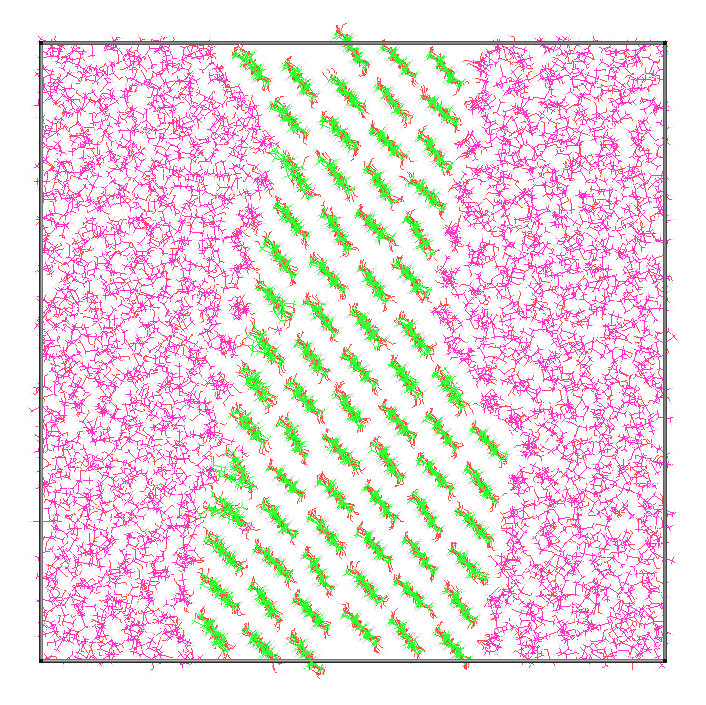
\includegraphics[height=0.75\textwidth]{cellulose_simulation_with_solvent_around_i/transition_with_eta_around.png}
        \end{minipage}
        \\
        \begin{minipage}[b]{0.12\textwidth}
            \centering
            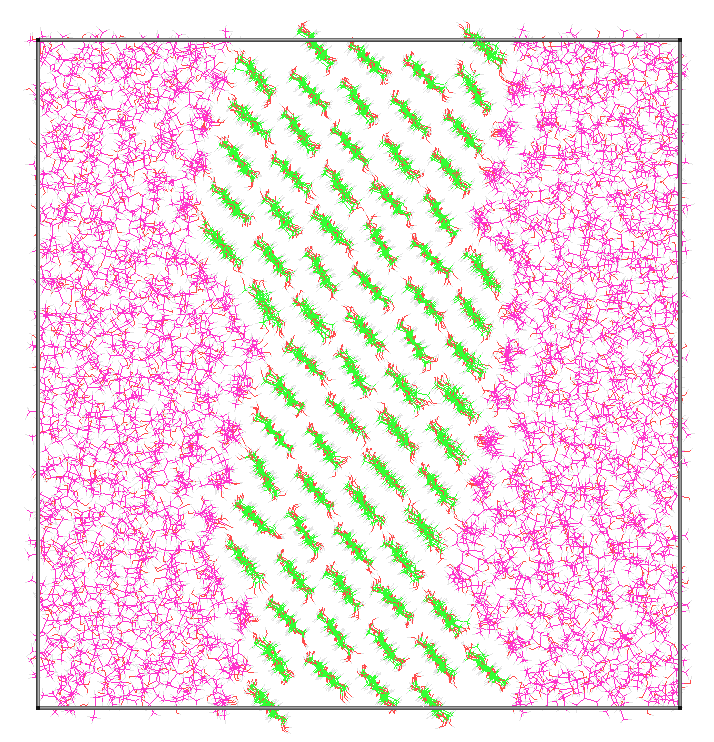
\includegraphics[height=0.75\textwidth]{cellulose_simulation_with_solvent_around_i/transition_with_ipa_around.png}
        \end{minipage}
        \begin{minipage}[b]{0.12\textwidth}
            \centering
            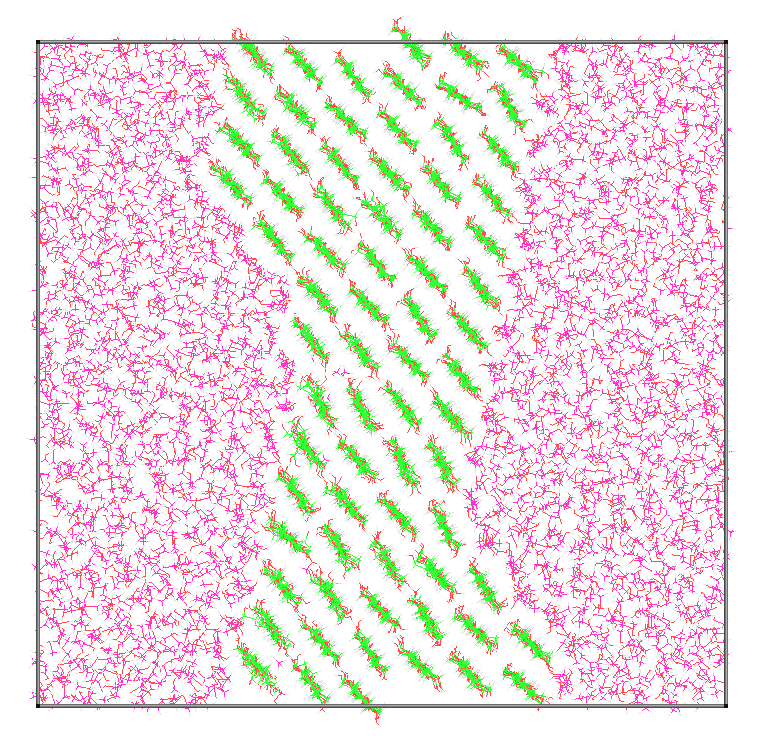
\includegraphics[height=0.75\textwidth]{cellulose_simulation_with_solvent_around_i/transition_with_mta_around.png}
        \end{minipage}
        \begin{minipage}[b]{0.12\textwidth}
            \centering
            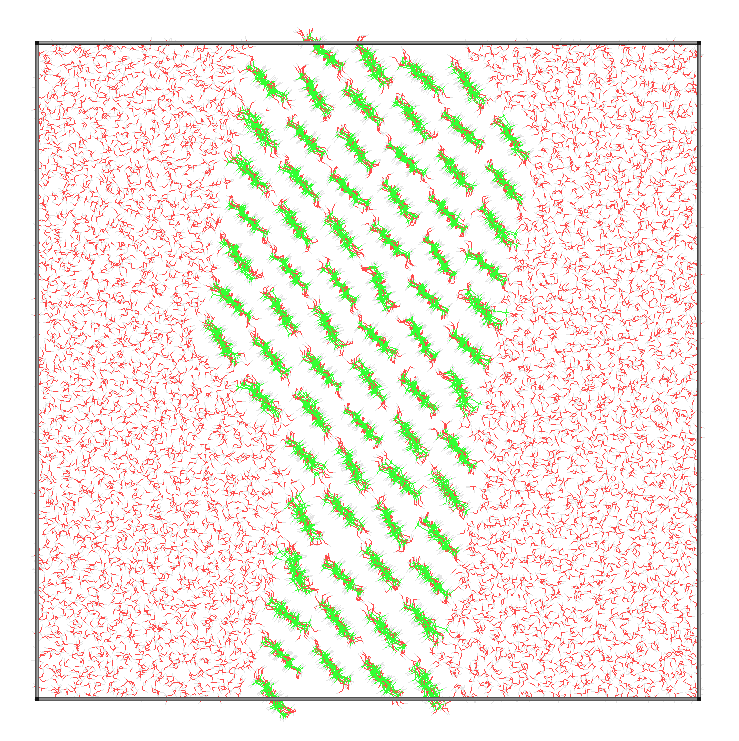
\includegraphics[height=0.75\textwidth]{cellulose_simulation_with_solvent_around_i/transition_with_sol_around.png}
        \end{minipage}
        \begin{minipage}[b]{0.12\textwidth}
            \centering
            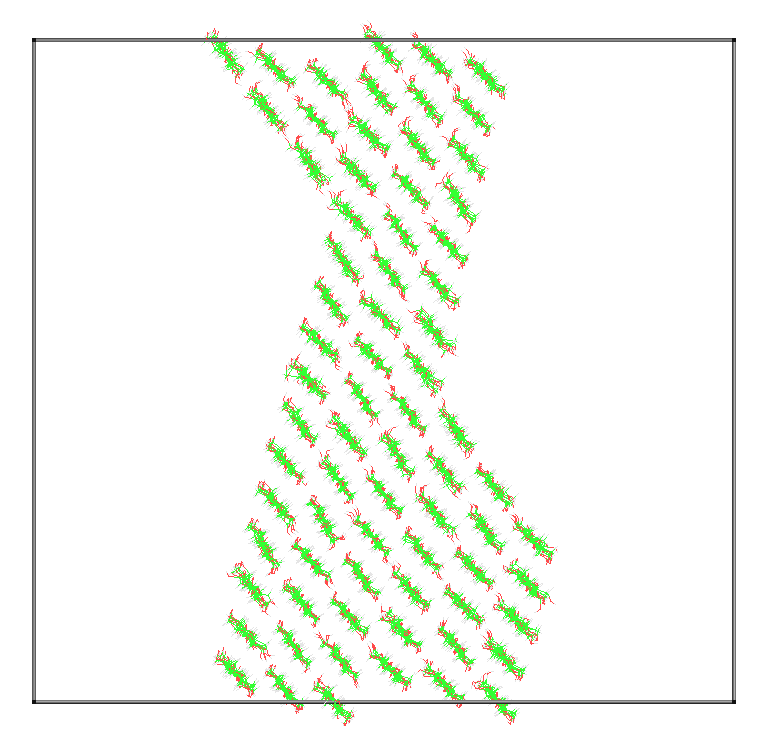
\includegraphics[height=0.75\textwidth]{cellulose_simulation_with_solvent_around_i/transition_with_none_around.png}
        \end{minipage}
        \subcaption{}
    \end{subfigure}
    \\
    \begin{subfigure}[b]{0.96\textwidth}
        \centering
        \begin{minipage}[b]{0.12\textwidth}
            \centering
            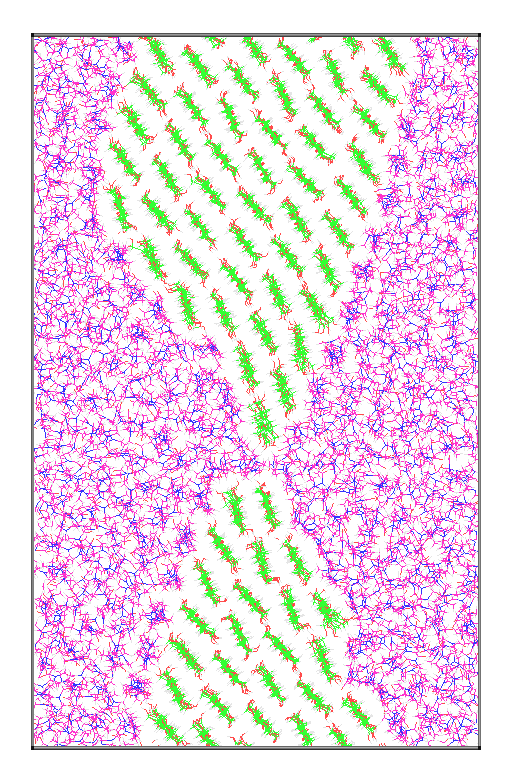
\includegraphics[height=0.93\textwidth]{cellulose_simulation_with_solvent_around_i/fracture_with_dmf_around.png}
        \end{minipage}
        \begin{minipage}[b]{0.12\textwidth}
            \centering
            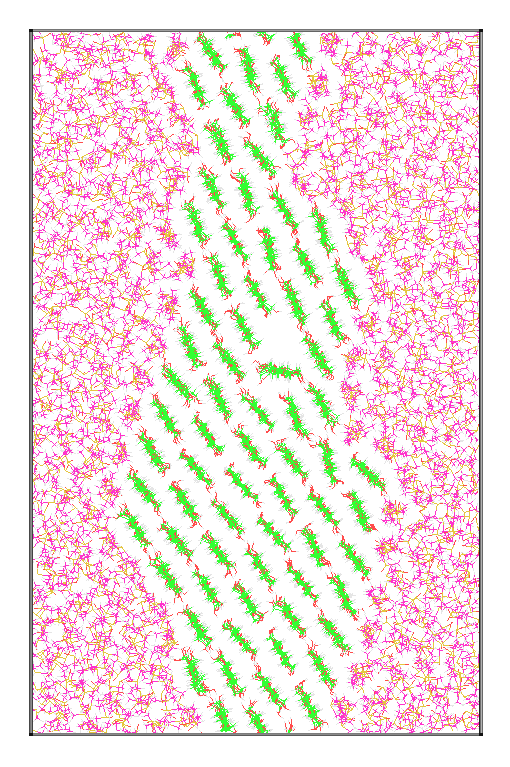
\includegraphics[height=0.93\textwidth]{cellulose_simulation_with_solvent_around_i/fracture_with_dmso_around.png}
        \end{minipage}
        \begin{minipage}[b]{0.12\textwidth}
            \centering
            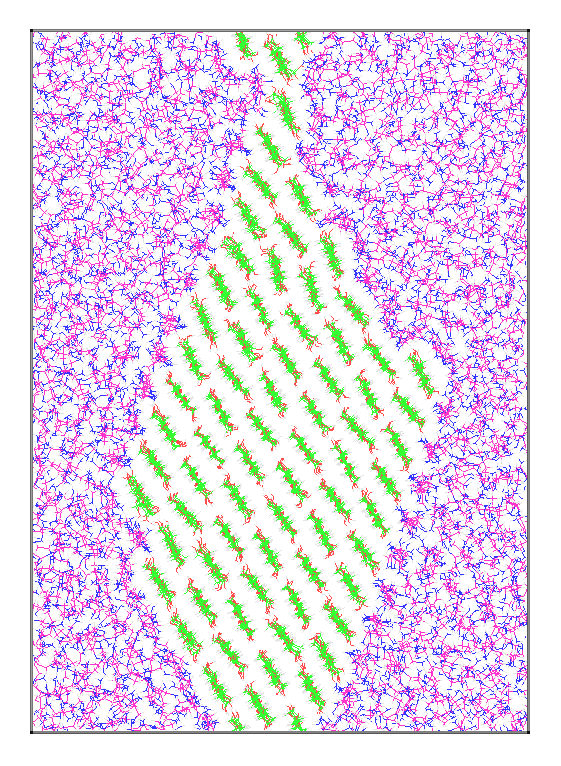
\includegraphics[height=0.93\textwidth]{cellulose_simulation_with_solvent_around_i/fracture_with_eda_around.png}
        \end{minipage}
        \begin{minipage}[b]{0.12\textwidth}
            \centering
            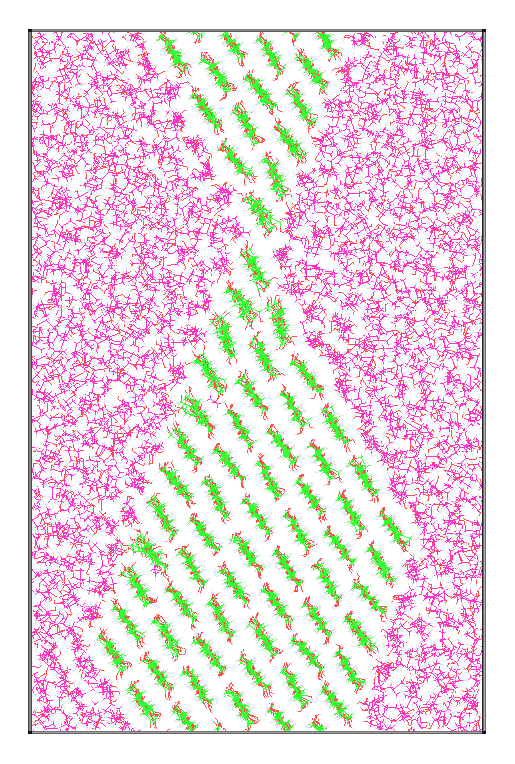
\includegraphics[height=0.93\textwidth]{cellulose_simulation_with_solvent_around_i/fracture_with_eta_around.png}
        \end{minipage}
        \\
        \begin{minipage}[b]{0.12\textwidth}
            \centering
            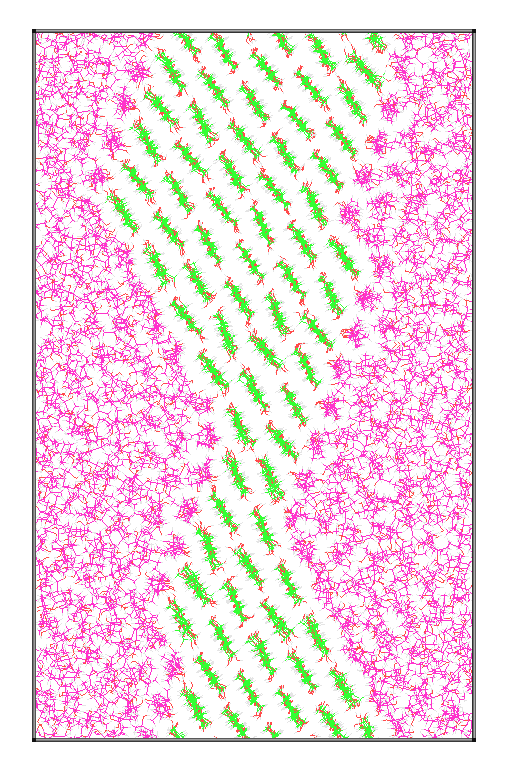
\includegraphics[height=0.93\textwidth]{cellulose_simulation_with_solvent_around_i/fracture_with_ipa_around.png}
        \end{minipage}
        \begin{minipage}[b]{0.12\textwidth}
            \centering
            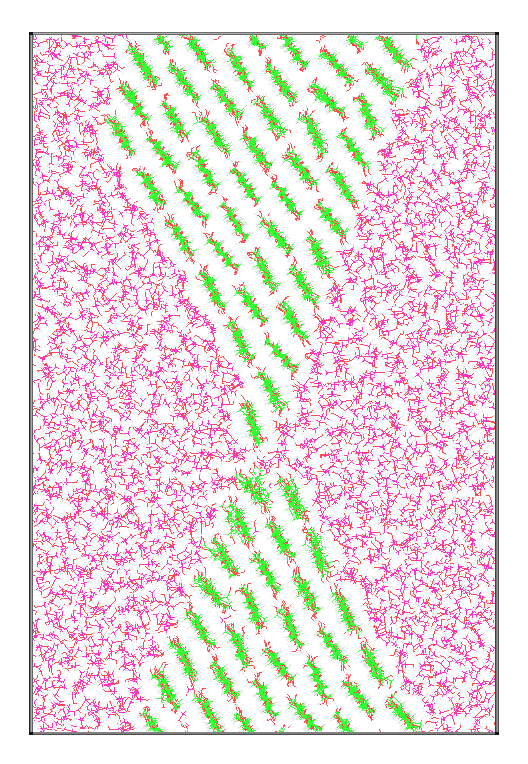
\includegraphics[height=0.93\textwidth]{cellulose_simulation_with_solvent_around_i/fracture_with_mta_around.png}
        \end{minipage}
        \begin{minipage}[b]{0.12\textwidth}
            \centering
            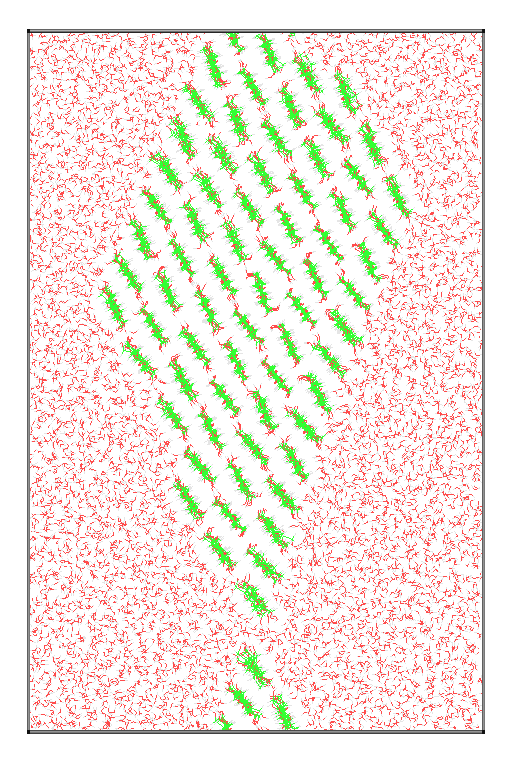
\includegraphics[height=0.93\textwidth]{cellulose_simulation_with_solvent_around_i/fracture_with_sol_around.png}
        \end{minipage}
        \begin{minipage}[b]{0.12\textwidth}
            \centering
            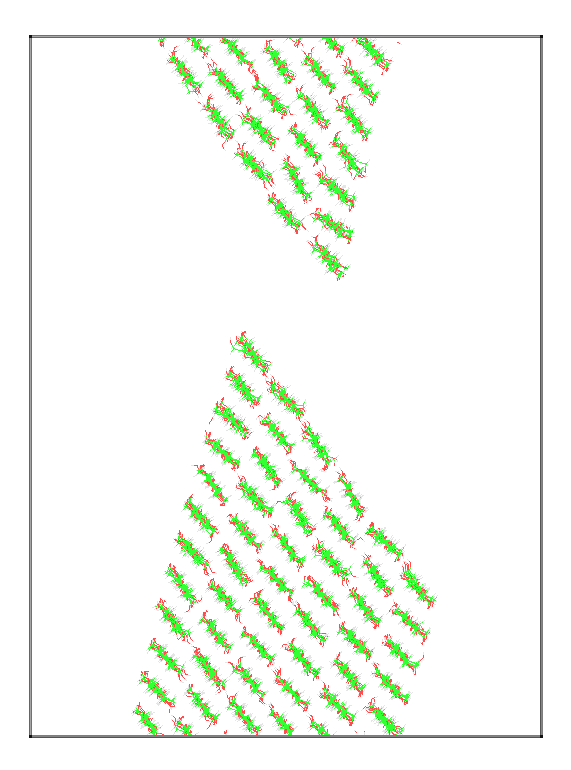
\includegraphics[height=0.93\textwidth]{cellulose_simulation_with_solvent_around_i/fracture_with_none_around.png}
        \end{minipage}
        \subcaption{}
    \end{subfigure}
    \captionsetup{font=scriptsize}
    \caption{
    Models and stretches of cellulose nanocrystals Type I surrounded by solvents on both sides.
    (a) Models surrounded by solvents on both sides, (b) intermediate structures of stretches, and (c) structures after stretches of the same strain.
    Models with DMF, DMSO, ethylenediamine (EDA), ethanol (ETA), isopropanol (IPA), methanol (MTA), water (SOL), and a solvent-free (NONE) control group were constructed.
    All of the were under NPT ensemble in xyz directions, except for the solvent-free group with only pressure in yz directions were controlled.
    The results elucidated that friction sliding remained important in solvent environments.
    Small polar molecules represented by EDA, MTA, and SOL exhibited strong erosive ability.
    }
    \label{fig:cellulose_nanocrystal_with_solvent_around_fractures}
\end{figure}

The solvent-free control group shows that even without a full periodicity, the friction sliding remained as the primary fracture behavior for the cellulose nanocrystals Type I, and this behaviors also persisted in the solvent environments.
Although the final morphologies of all the models were similar, by comparing the intermediate structures during loading,
it can be observed that small polar molecules (such as EDA, MTA, and SOL) had stronger erosive abilities on cellulose nanocrystals, promoting the friction sliding phenomenon at the interfaces.
As a molecule with a relatively large size and weak polarity, DMSO has a weaker erosive ability on cellulose nanocrystals Type I, and improve the ductility and toughness comparing to the other solvents.
Quantitative strength and toughness data are shown in Figure \ref{fig:cellulose_nanocrystal_with_solvent_around_performance}.
These simulation data indicate that the size and polarity of solvent molecules are key factors affecting the performances and phenomena of cellulose nanocrystals Type I in the solvent environments.
This is related to the crucial influences of hydrogen bonding and Coulomb interactions during the stretches of the cellulose nanocrystals Type I.

\begin{figure}[htbp]
    \centering
    \begin{subfigure}[b]{0.96\textwidth}
        \centering
        \begin{minipage}[b]{0.12\textwidth}
            \centering
            
\includegraphics[height=0.60\textwidth]{cellulose_simulation_with_solvent_around_ii/relaxation_with_dmf_around.png}
        \end{minipage}
        \begin{minipage}[b]{0.12\textwidth}
            \centering
            
\includegraphics[height=0.60\textwidth]{cellulose_simulation_with_solvent_around_ii/relaxation_with_dmso_around.png}
        \end{minipage}
        \begin{minipage}[b]{0.12\textwidth}
            \centering
            
\includegraphics[height=0.60\textwidth]{cellulose_simulation_with_solvent_around_ii/relaxation_with_eda_around.png}
        \end{minipage}
        \begin{minipage}[b]{0.12\textwidth}
            \centering
            
\includegraphics[height=0.60\textwidth]{cellulose_simulation_with_solvent_around_ii/relaxation_with_eta_around.png}
        \end{minipage}
        \\
        \begin{minipage}[b]{0.12\textwidth}
            \centering
            
\includegraphics[height=0.60\textwidth]{cellulose_simulation_with_solvent_around_ii/relaxation_with_ipa_around.png}
        \end{minipage}
        \begin{minipage}[b]{0.12\textwidth}
            \centering
            
\includegraphics[height=0.60\textwidth]{cellulose_simulation_with_solvent_around_ii/relaxation_with_mta_around.png}
        \end{minipage}
        \begin{minipage}[b]{0.12\textwidth}
            \centering
            
\includegraphics[height=0.60\textwidth]{cellulose_simulation_with_solvent_around_ii/relaxation_with_sol_around.png}
        \end{minipage}
        \begin{minipage}[b]{0.12\textwidth}
            \centering
            
\includegraphics[height=0.60\textwidth]{cellulose_simulation_with_solvent_around_ii/relaxation_with_none_around.png}
        \end{minipage}
        \subcaption{}
    \end{subfigure}
    \\
    \begin{subfigure}[b]{0.96\textwidth}
        \centering
        \begin{minipage}[b]{0.12\textwidth}
            \centering
            
\includegraphics[height=0.77\textwidth]{cellulose_simulation_with_solvent_around_ii/transition_with_dmf_around.png}
        \end{minipage}
        \begin{minipage}[b]{0.12\textwidth}
            \centering
            
\includegraphics[height=0.77\textwidth]{cellulose_simulation_with_solvent_around_ii/transition_with_dmso_around.png}
        \end{minipage}
        \begin{minipage}[b]{0.12\textwidth}
            \centering
            
\includegraphics[height=0.77\textwidth]{cellulose_simulation_with_solvent_around_ii/transition_with_eda_around.png}
        \end{minipage}
        \begin{minipage}[b]{0.12\textwidth}
            \centering
            
\includegraphics[height=0.77\textwidth]{cellulose_simulation_with_solvent_around_ii/transition_with_eta_around.png}
        \end{minipage}
        \\
        \begin{minipage}[b]{0.12\textwidth}
            \centering
            
\includegraphics[height=0.77\textwidth]{cellulose_simulation_with_solvent_around_ii/transition_with_ipa_around.png}
        \end{minipage}
        \begin{minipage}[b]{0.12\textwidth}
            \centering
            
\includegraphics[height=0.77\textwidth]{cellulose_simulation_with_solvent_around_ii/transition_with_mta_around.png}
        \end{minipage}
        \begin{minipage}[b]{0.12\textwidth}
            \centering
            
\includegraphics[height=0.77\textwidth]{cellulose_simulation_with_solvent_around_ii/transition_with_sol_around.png}
        \end{minipage}
        \begin{minipage}[b]{0.12\textwidth}
            \centering
            
\includegraphics[height=0.77\textwidth]{cellulose_simulation_with_solvent_around_ii/transition_with_none_around.png}
        \end{minipage}
        \subcaption{}
    \end{subfigure}
    \\
    \begin{subfigure}[b]{0.96\textwidth}
        \centering
        \begin{minipage}[b]{0.12\textwidth}
            \centering
            
\includegraphics[height=0.95\textwidth]{cellulose_simulation_with_solvent_around_ii/fracture_with_dmf_around.png}
        \end{minipage}
        \begin{minipage}[b]{0.12\textwidth}
            \centering
            
\includegraphics[height=0.95\textwidth]{cellulose_simulation_with_solvent_around_ii/fracture_with_dmso_around.png}
        \end{minipage}
        \begin{minipage}[b]{0.12\textwidth}
            \centering
            
\includegraphics[height=0.95\textwidth]{cellulose_simulation_with_solvent_around_ii/fracture_with_eda_around.png}
        \end{minipage}
        \begin{minipage}[b]{0.12\textwidth}
            \centering
            
\includegraphics[height=0.95\textwidth]{cellulose_simulation_with_solvent_around_ii/fracture_with_eta_around.png}
        \end{minipage}
        \\
        \begin{minipage}[b]{0.12\textwidth}
            \centering
            
\includegraphics[height=0.95\textwidth]{cellulose_simulation_with_solvent_around_ii/fracture_with_ipa_around.png}
        \end{minipage}
        \begin{minipage}[b]{0.12\textwidth}
            \centering
            
\includegraphics[height=0.95\textwidth]{cellulose_simulation_with_solvent_around_ii/fracture_with_mta_around.png}
        \end{minipage}
        \begin{minipage}[b]{0.12\textwidth}
            \centering
            
\includegraphics[height=0.95\textwidth]{cellulose_simulation_with_solvent_around_ii/fracture_with_sol_around.png}
        \end{minipage}
        \begin{minipage}[b]{0.12\textwidth}
            \centering
            
\includegraphics[height=0.95\textwidth]{cellulose_simulation_with_solvent_around_ii/fracture_with_none_around.png}
        \end{minipage}
        \subcaption{}
    \end{subfigure}
    \captionsetup{font=scriptsize}
    \caption{
    Models and stretches of cellulose nanocrystals Type II surrounded by solvents on both sides.
    (a) Models surrounded by solvents on both sides, (b) intermediate structures of stretches, and (c) structures after stretches of the same strain.
    Models with DMF, DMSO, ethylenediamine (EDA), ethanol (ETA), isopropanol (IPA), methanol (MTA), water (SOL), and a solvent-free (NONE) control group were constructed.
    All of the were under NPT ensemble in xyz directions, except for the solvent-free group with only pressure in yz directions were controlled.
    In solvent environments, the restructure toughening of non-fully periodic Type II nanocrystals decreased significantly.
    The dependency of fully periodic crystal structure for better strength and toughness of Type II was further confirmed.
    Small polar molecules represented by ethylenediamine (EDA), methanol (MTA), and water (SOL) exhibit strong erosive ability.
    }
    \label{fig:cellulose_nanocrystal_ii_with_solvent_around_fractures}
\end{figure}

Using the same modelling procedure, pressure control, and stretch speed, cellulose nanocrystal Type II were simulated subjected to same treatments (Figure \ref{fig:cellulose_nanocrystal_ii_with_solvent_around_fractures}).
The results of the solvent-free control group showed that in a non-fully-periodic situation, cellulose nanocrystals Type II cannot undergo complex restructure or correspondingly exhibit high toughness.
Even so, cellulose nanocrystals Type II still formed laminar structures after fractures.

\begin{figure}[htbp]
    \centering
    \begin{subfigure}[b]{0.48\textwidth}
        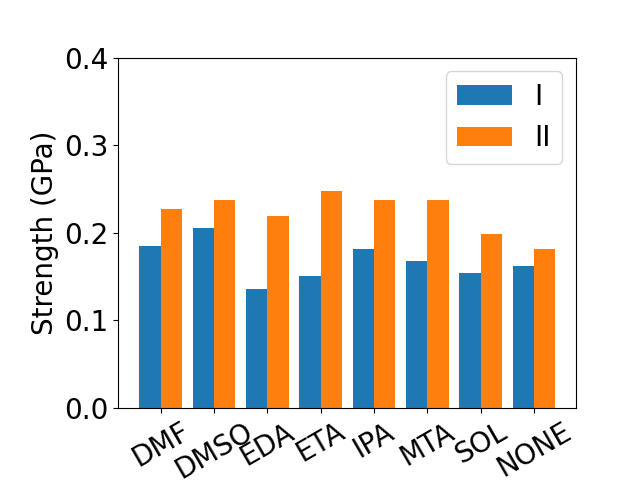
\includegraphics[width=0.96\textwidth]{cellulose_simulation_with_solvent_around_i/stretch_strength_around_with_solvent.png}
        \subcaption{}
    \end{subfigure}
    \begin{subfigure}[b]{0.48\textwidth}
        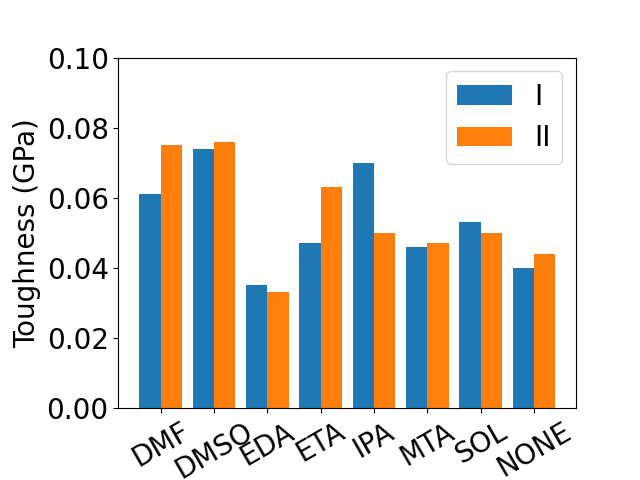
\includegraphics[width=0.96\textwidth]{cellulose_simulation_with_solvent_around_ii/stretch_toughness_around_with_solvent.png}
        \subcaption{}
    \end{subfigure}
    \captionsetup{font=scriptsize}
    \caption{
    Mechanical properties of cellulose nanocrystals surrounded by solvents on both sides.
    (a) Strength and (b) toughness with solvent type and cellulose nanocrystal configuration.
    In overall, Type I crystals still exhibited friction sliding phenomenon and have lower strength in this specific solvent scenario comparing to the Type II.
    The restructure toughening mechanism of Type II was heavily dependent on an ideal crystal structure, which was not presented here.
    Small polar molecules represented by ethylenediamine (EDA), methanol (MTA), and water (SOL) exhibit strong erosive ability, corresponding to the lowest structural toughness.
    Other molecules represented by DMSO, which are slightly larger and less polar, can enhance toughness.
    }
    \label{fig:cellulose_nanocrystal_with_solvent_around_performance}
\end{figure}

The intermediate structures and fractures shown in Figure \ref{fig:cellulose_nanocrystal_with_solvent_around_performance} further illustrated the impact of solvent polarity and molecule size on fracture behaviors.
EDA, MTA, SOL, and the slightly larger IPA still exhibited strong erosive ability, capable of promoting horizontal dislocations and fractures of Type II nanocrystals as shown in the intermediate structures.
Molecules represented by DMSO, which are weaker in polarity and slightly larger in volume, still contributed to increase the ductility of cellulose nanocrystals Type II, protecting rather than promoting fractures.
However, the behavior of water differed from the that in the Type I.
As a typical small polar molecules, water molecules did not promote dislocation in the Type II; instead, they tended to promote local rotation and overall tension.
That should be related to the more exposure of cellulose hydroxyls to the water molecules in this case.
Therefore, the local horizontal dislocation was not evident in the intermediate state by water, and the final fracture structure exhibits more dislocations.

By quantitatively comparing the mechanical properties of cellulose nanocrystals Type I and Type II surrounded by solvents on both sides,
it was noted that small polar molecules represented by ethylenediamine (EDA), methanol (MTA), and water (SOL) can reduce the toughness during the stretches, while molecules with weaker polarity and slightly larger volumes, such as DMSO, can increase the toughness.
With the solvents surrounded on both sides, the strength of cellulose nanocrystals was not significantly affected.
Cellulose nanocrystals Type I, influenced by their unique friction sliding, represented lower strength compared to the Type II.

\section*{Discussion}
\addtocounter{section}{1}
\setcounter{subsection}{0}
\addcontentsline{toc}{section}{\protect\numberline{}Discussion}\indent

As a new type of cellulose materials, cellulose nanocrystals is green, widely available, and owns excellent performances.
To design advanced cellulose materials, a full understanding of the properties of cellulose materials on a microscopic scale was necessary.
The research topics in this study, anisotropy\cite{wu2014tensile}, fracture behaviors\cite{wu2013atomistic,zhang2021hydrogen}, configuration transformation\cite{chundawat2011restructuring,el2011crystal,kobayashi2011crystal,miyamoto2015molecular,kugo2024elucidating}, size dependency\cite{sinko2014dimensions}, solvents effects\cite{wang2020highly,he2021effects,fink2001structure}, and structural design\cite{tu2021superior,chen2020electric,li2021ionic} of cellulose nanocrystals were all partially addressed in the previous studies.
Owing the stable properties of the very strong covalent bonds along the chain, this study focused on the transverse anisotropy, stressing the 3D structures of cellulose nanocrystals.
It is not only a fiber materials, it is also strong and active along the chains or along the interface of the nanocrystals.
This study emphasized on the mechanical of nanocrystals, further extended these topics, and systematical comparisons involving characteristic directions and varying solvents were made.
Based on the anisotropy and size dependency, we proposed a toughening mechanism by transverse arrangements.

The extension included several points:
1. except for the researches involving configuration transformations, the previous studies usually focused on the cellulose nanocrystals Type I only.
However, the cellulose nanocrystals Type II were emphasized equivalently in this study.
2. for anisotropy and fracture behaviors, this study bypassed the technical difficulty of apply shearing loads in molecular dynamics by constructing models in the characteristic directions, and the cell deformation method with full pressure control made it possible to better address the mechanical performances of cellulose nanocrystals.
As a result, the mechanical performances and frictional sliding phenomenon of the slant models of the Type I were presented.
And the possible restructure of the slant models of the Type II were also illustrated.
This special fracture behaviors were the base for the following toughening designs.
3. for configuration transformations, we found that the structure of cellulose nanocrystals II could be induced to laminar structure similar to the Type II only the external mechanical loads, as the fracture behaviors of its Type I elucidated.
Considering the configuration transformation requirement for extraction from plants and material performance tuning, this may be helpful for future researches.
4. for the size dependency, we gave an quantitative explanation by delta potential energy per unit volume.
The inspiration and morphological phenomenon for that is, we noticed the fracture behaviors of were localized.
As an assumption the contribution of the localized fracture behaviors in larger models should be lower, and proved by the delta potential energy density.
5. for the solvent effects, our perspective also had its uniqueness.
For the previous studies, the cellulose nanocrystals molecules were accompanied or fully surrounded by solvent molecules, and only few studied emphasized the wetting (the solvents entered the gaps of chains and became part of the crystals)\cite{malaspina2019molecular,uto2019molecular}.
In this study, the solvents were not placed on the only x direction (the left and right sides of the cellulose nanocrystals), while the y and z directions of cellulose nanocrystals were still periodic to itself.
Thereby, the simulations about solvents concentrated purely on the solvent-nanocrystal interfaces influences on the mechanical performances of nanocrystals, whether erosive or protective.
The erosive effects from small polar molecules such as water and EDA was fully within expectations, as they could interact with the hydroxyls using hydrogen bonds and Coulomb interactions and promote dismantle.
However, the lager (in molecular size) and weaker (in polarity) molecule such as DMSO exhibit protective phenomena, as they could delay the sliding behaviors of both the Type I and Type II.

These above points were only the further demonstration of existing researches.
The transverse arrangement toughening patterns were somehow original contributions from this studies.
After understanding the frictional sliding and size dependency of the cellulose nanocrystals Type I, we realized that maybe arrange unit blocks in a non-crystal pattern may help improve the ductility and toughness of the whole structure.
Inspired by the twin structures, symmetric and cross patterns were designed and examined.
They hindered the friction sliding and promote localize rotations, benefiting the overall ductility.
This toughening mechanism may help future advanced design of cellulose nanocrystals structure design and utilization.

However, significant inherent shortcomings still exist for this model.
First, limited the computation resources and lack of experiment verifications, the simulations here were limited to a relatively small size, and the applicability of mechanisms of solvents and toughening may be more limited in practical cellulose materials.
And the solvents we considered are limited and may be still insufficient.
On the other hand, although some delicate methods to operate cellulose chains such as cross-linking\cite{tu2021superior} and alignment\cite{chen2020electric,li2021ionic} were already developed,
we are kind of pessimistic about the implement difficulty of such a fine control for cellulose nanocrystals as we did in simulations.
Anyway, we wish this fundamental and pioneering study would still be help for further understanding and development of cellulose nanocrystals.

\section*{Conclusions}
\addtocounter{section}{1}
\setcounter{subsection}{0}
\addcontentsline{toc}{section}{\protect\numberline{}Conclusions}\indent

In this study, a series of cellulose nanocrystals models were constructed and simulated, addressing the anisotropy, solvent effects, and toughening mechanism designs for both Type I and Type II.
To overcome the technical difficulty of applying shearing loads and the well known strong covalent bonds along the chain, models were constructed based on the characteristic directions in the cross section.
The important frictional sliding of the cellulose nanocrystals Type I was presented, which is contributed by the laminar structure and hydrogen bonds by side chains.
For the cellulose nanocrystals Type II, it could exhibit both the brittle behavior or restructure-based more tough fractures.
The restructure of the Type II led to a laminar fracture similar to the Type I, thus may be exploited as a configuration transformation mechanism purely induced by mechanical loads.
These fracture behaviors were further confirmed by replica simulations among varying loading speeds.
Inspired by the previous researches on the size effects on the cellulose nanocrystals Type I, we examined the size dependency of cellulose nanocrystals for both the Type I and Type II, and found that small cellulose nanocrystals could exhibit better ductility and toughness.
Then, an quantitative explanation for the size dependency was given by the delta potential energy density, as the localized fracture behaviors suggested.
After understanding the fracture behaviors and size dependency, symmetric and cross arrangement patterns were proposed and proved for its toughening effects.
We also checked the solvent effects from out own perspective, as the solvent is strictly outside and surrounded the cellulose nanocrystals, which is a specific load case concentrating on the solvent effects on the nanocrystals.
Our results in the solvent environment confirmed that the small and polar molecule are able to interfere the side chain hydroxyls and sliding fractures for both the Type I and Type II, while the larger and less polar molecule could delay the fractures and protect the nanocrystals.
For the limited comparisons, later simulations and experiments could further enhance the scope and deepness of this study.
With the development of material design and preparation, these results requiring delicate operations may be practically implemented and help future cellulose material development.

\section*{Conflict of Interest declaration}
\addtocounter{section}{1}
\setcounter{subsection}{0}
\addcontentsline{toc}{section}{\protect\numberline{}Conflict of Interest declaration}\indent

The author declares no competing financial interest.

\section*{Data availability}
\addtocounter{section}{1}
\setcounter{subsection}{0}
\addcontentsline{toc}{section}{\protect\numberline{}Data availability}\indent

The training data, models, simulation codes, processed data, plot scripts, and latest manuscript are available at

$\textrm{https://github.com/EiPiFun/cll-transverse-data}$

\noindent
. The raw data, pre-processing codes, and post-processing codes are available upon requests.

\section*{Acknowledgments}
\addtocounter{section}{1}
\setcounter{subsection}{0}
\addcontentsline{toc}{section}{\protect\numberline{}Acknowledgments}\indent

Xu Dong thanks the Department of Engineering Mechanics of Zhejiang University for the funding and computational resources.

\section*{Author Contributions}
\addtocounter{section}{1}
\setcounter{subsection}{0}
\addcontentsline{toc}{section}{\protect\numberline{}Author Contributions}\indent

Xu Dong: Conceptualization, Data curation, Formal analysis, Investigation, Methodology, Project administration, Resources, Software, Validation, Visualization, Writing - original draft, Writing - review \& editing.

A professor from the Department of Engineering Mechanics of Zhejiang University provided some additional Methodology, Resources, and Writing - review \& editing helps and chose to be anonymous.
%\\\\
%\noindent\Large{\textbf{References}}
%\newsavebox{\tempbib}
%\savebox{\tempbib}{\parbox{\textwidth}{
%\bibliography{cll_transverse_references}
%}}

\linespread{1.0}\footnotesize\bibliography{cll_transverse_references}
\addtocounter{section}{1}
\setcounter{subsection}{0}
\addcontentsline{toc}{section}{\protect\numberline{}References}





\setcounter{section}{0}
\setcounter{subsection}{0}

\setcounter{table}{0}
\setcounter{figure}{0}
\setcounter{equation}{0}

\renewcommand{\thesection}{S\arabic{section}}
\renewcommand{\thesubsection}{S\arabic{subsection}}

\renewcommand{\thetable}{S\arabic{table}}
\renewcommand{\thefigure}{S\arabic{figure}}
\renewcommand{\theequation}{S\arabic{equation}}





\section*{Supplementary Information}
\addtocounter{section}{1}
\setcounter{subsection}{0}
\addcontentsline{toc}{section}{\protect\numberline{}Supplementary Information}\indent

\normalsize The following subsections and data are included in the Supplementary Information.
\\\indent

Models and relaxations of cellulose nanocrystals Type I

Hydrogen bond number and potential energy during stretches of the Type I

Models and relaxations of cellulose nanocrystals Type II

Hydrogen bond number and potential energy during stretches of the Type II

Stretch transitions of cellulose nanocrystals Type II larger model

Transverse arrangement patterns fractures of the Type I with more unit blocks

Simulations of different size models and size dependency of cellulose nanocrystals Type II

Transverse arrangement patterns of the Type II
\\\indent

\refstepcounter{figure}\label{fig:cellulose_nanocrystal_structure_and_models}\figurename\quad\thefigure,\quad
\refstepcounter{figure}\label{fig:cellulose_nanocrystal_relaxations}\figurename\quad\thefigure,\quad
\refstepcounter{figure}\label{fig:cellulose_nanocrystal_stretch_hydrogen_bond_number_and_energy}\figurename\quad\thefigure,\quad
\refstepcounter{figure}\label{fig:cellulose_nanocrystal_ii_structure_and_models}\figurename\quad\thefigure,\quad

\refstepcounter{figure}\label{fig:cellulose_nanocrystal_ii_relaxations}\figurename\quad\thefigure,\quad
\refstepcounter{figure}\label{fig:cellulose_nanocrystal_ii_larger_stretch_transitions}\figurename\quad\thefigure,\quad
\refstepcounter{figure}\label{fig:cellulose_nanocrystal_ii_stretch_hydrogen_bond_number_and_energy}\figurename\quad\thefigure,\quad
\refstepcounter{figure}\label{fig:cellulose_nanocrystal_more_transverse_arrangement_fractures}\figurename\quad\thefigure,\quad

\refstepcounter{figure}\label{fig:cellulose_nanocrystal_ii_size_dependency}\figurename\quad\thefigure,\quad
\refstepcounter{figure}\label{fig:cellulose_nanocrystal_ii_delta_energy_density_with_size}\figurename\quad\thefigure,\quad
\refstepcounter{figure}\label{fig:cellulose_nanocrystal_ii_transverse_arrangement_fractures}\figurename\quad\thefigure,\quad
\refstepcounter{figure}\label{fig:cellulose_nanocrystal_ii_more_transverse_arrangement_fractures}\figurename\quad\thefigure,\quad
\refstepcounter{figure}\label{fig:cellulose_nanocrystal_ii_transverse_arrangement_performance_with_patterns}\figurename\quad\thefigure,\quad

\end{document}

